\documentclass[11pt, a4paper]{article}

\usepackage[utf8]{inputenc}
\usepackage{graphicx}
\graphicspath{ {images/} }
\usepackage{mathtools}
\usepackage{amssymb}
\usepackage{amsmath}
\usepackage[ngerman,english]{babel}
\usepackage{cite}
\usepackage{bibgerm}
\usepackage{fullpage}
\usepackage[top=1.5cm,bottom=1.5cm,left=3.5cm,right=2.5cm,headsep=1.5cm,includeheadfoot]{geometry}
\usepackage{tabularx}
\usepackage{caption}
\usepackage{subcaption}
\usepackage{eurosym}
\usepackage{enumitem}
\usepackage{multicol}
\usepackage{tikz}
\usepackage{tkz-euclide}
\usepackage{pgfplots}
\usepackage{pdflscape}
\usepackage{acronym}
\usepackage{blindtext}
\usepackage{ifthen}
\usepackage{setspace}
\usepackage{cancel}
\usepackage{color}
\usepackage{listings}
\usepackage{comment}
\usepackage{xcolor}
\usepackage{colortbl}
\usepackage[parfill]{parskip}
\usepackage{url}

\usepackage{fancyhdr}
\pagestyle{fancy}

\fancyhf{} % clear all
\fancyhead[L]{\leftmark}
\fancyfoot[C]{-- \thepage{} --}
\setlength{\headheight}{0pt}
\renewcommand{\headrulewidth}{0.5pt}
\renewcommand{\footrulewidth}{0pt}
\setlength{\skip\footins}{0.7cm}

\usetikzlibrary{shapes.geometric}
\usetikzlibrary{graphs}
\usetikzlibrary{positioning}

\onehalfspacing
\setlength\parindent{0pt}

%\everymath{\displaystyle}

\allowdisplaybreaks

\definecolor{AI-BLUE}{rgb}{0,0.57,0.87}
\definecolor{lightgray}{rgb}{0.91,0.91,0.91}

% Eigene Befehle
\newcommand\q[1]{\emph{"#1"}}
\renewcommand\equiv{\Leftrightarrow}
\newcommand\vertequal[2]{\underset{\underset{#2}{\parallel}}{#1}}
\newcommand\cif{\text{if }}
\newcommand\abs[1]{\left|#1\right|}
\newcommand\norm[1]{\abs{\abs{#1}}}
\newcommand\diff[1]{\text{ d#1}}
\newcommand\av[1]{\left\langle#1\right\rangle}
\newcommand\ev[1]{\mathbb{E}\left(#1\right)}
\newcommand\br[1]{\left(#1\right)}
\newcommand\ubr[2]{\underbrace{#1}_{#2}}
\newcommand\quer[1]{\overline{#1}}
\newcommand\setequal{\overset{!}{=}}
\newcommand\dint{\displaystyle \int}
\newcommand\dsum{\displaystyle \sum}
\newcommand\dprod{\displaystyle \prod}
\newcommand\closedInt[2]{\left[#1,#2\right]}
\newcommand{\checkbox}{\Large \Square \normalsize \hspace{0.4cm}}
\newcommand\V[1]{\ensuremath{\underline{\mathbf{#1}}}}
\newcommand\M[1]{\ensuremath{\underline{\underline{\mathbf{#1}}}}}
\newcommand\myref[1]{\ref{#1} (p. \pageref{#1})}
\newcommand\myrefcomma[1]{\ref{#1}, p. \pageref{#1}}

\begin{document}

\thispagestyle{empty}

\setlength{\hoffset}{-0.5cm} % center title page

\lstset{
  basicstyle=\small,           % the size of the fonts that are used for the code
  breaklines=true,             % sets automatic line breaking
  captionpos=b,                % sets the caption-position to bottom
  frame=single,                % adds a frame around the code
  keepspaces=true,             % keeps spaces in text, useful for keeping indentation of code (possibly needs columns=flexible)
  numbers=right,               % where to put the line-numbers; possible values are (none, left, right)
  showspaces=false,            % show spaces everywhere adding particular underscores; it overrides 'showstringspaces'
  stepnumber=1,                % the step between two line-numbers. If it's 1, each line will be numbered
  tabsize=4,                   % sets default tab size to 4 spaces
  xleftmargin=0.14cm		   % sets left margin
}

\begin{titlepage}
    \begin{center}
    \LARGE \textbf{Master's Thesis}\\
    \vspace{3cm}
    \normalsize
    Master's Thesis\\
    in the Program of Applied Computer Science\\
    at the Ruhr-University Bochum\\
    at the Institute for Neural Computation\\
    in the Summer Term 2016\\
    \vspace{3cm}
    \LARGE \textbf{A Deep Convolutional Network for Facial Landmark Estimation} \\
    %\LARGE \textbf{A Gabor Wavelet Based Convolutional Neural Network for Facial Landmark Estimation} \\
    \vspace{3cm}
    \normalsize
    \textbf{Author:}\\
    Schrör, Phil Yannick\\
    108 011 214 024\\
    \vspace{2cm}
    \textbf{Submission Date:}\\
    31st of October 2016\\
    \vspace{2cm}
    \textbf{Supervisors:}\\
    PD Dr. Rolf P. Würtz\\
    M.Sc. Andreas Nilkens
    \end{center}
\end{titlepage}

\newpage
\pagenumbering{Roman}
\setcounter{page}{2}

\tableofcontents

\newpage

\addcontentsline{toc}{section}{List of Acronyms}

\section*{List of Acronyms}
\markboth{LIST OF ACRONYMS}{}

The following list provides an overview about all abbreviations, which are used in this thesis. When an abbreviated term is mentioned for the first time, its whole name is written out next to its abbreviation in parentheses. From the second time on only the abbreviation will be displayed.\\

\renewcommand*\bflabel[1]{\textbf{#1}}
\begin{acronym}[INDENT]
\acro{ANN}{Artificial Neural Network}
\acro{CNN}{Convolutional Neural Network}
\acro{CPU}{Central Processing Unit}
\acro{GPU}{Graphics Processing Unit}
\acro{HDF}{Hierarchical Data Format}
\acro{MSSE}{Mean Summed Squared Error}
\acro{MUCT}{Milborrow / University of Cape Town} (Image data set)
\acro{PIL}{Python Imaging Library}
\acro{ReLU}{Rectified Linear Unit}
\acro{RGB}{Red-Green-Blue} (Color space)
\acro{RNN}{Recurrent Neural Network}
\acro{SGD}{Stochastic Gradient Descent}
\end{acronym}


\newpage

\setcounter{page}{1}
\pagenumbering{arabic}

%%%%%%%%%%%%%%%%%%%%%%%%%%%%%%%%%%%%%%%%%%%%%%%%%%%%%%%%%%%%%%%%%%%%%%%%%%%%%%%%%%%%%%%%%%%%%%%%%%%%%%%%%
%%%%%%%%%%%%%%%%%%%%%%%%%%%%%%%%%%%%%%%%%%%%%%%%%%%%%%%%%%%%%%%%%%%%%%%%%%%%%%%%%%%%%%%%%%%%%%%%%%%%%%%%%
%									INTRODUCTION CHAPTER BEGINS HERE									%
%%%%%%%%%%%%%%%%%%%%%%%%%%%%%%%%%%%%%%%%%%%%%%%%%%%%%%%%%%%%%%%%%%%%%%%%%%%%%%%%%%%%%%%%%%%%%%%%%%%%%%%%%
%%%%%%%%%%%%%%%%%%%%%%%%%%%%%%%%%%%%%%%%%%%%%%%%%%%%%%%%%%%%%%%%%%%%%%%%%%%%%%%%%%%%%%%%%%%%%%%%%%%%%%%%%

\section{Introduction}

\acp{ANN} have proven to be very powerful tools developed and used in the field of Neural Computation. Particularly, \acp{CNN} exhibit a solid performance on graphical data like images or videos. Finding to a lesser or greater extent apparent patterns and structures in images can be very useful in many respects, one of them being the diagnosis of diseases which influence the appearance of the human face\footnote{cf. \cite{ebgm}}. For that reason \acp{CNN} are used in the scope of this thesis to estimate the position of so called landmarks in images of human faces. While some of those landmarks are preeminent features like the eyes or the tip of the nose, other landmarks are less prominent points like the contours of the chin, which are harder to find.\\
Since tagging all those landmarks by hand is tedious work, it is desirable to create an automatism which estimates them. In order to reach this goal two different general network architectures are examined and tested in many different configurations. Both kinds of network take a \ac{RGB}-image of a human face as input and produce the estimated coordinates of the landmarks as output. The first approach trains a complete \ac{CNN} conventionally, i.e. all the network's weights are initialized randomly and subsequently trained by the \ac{SGD} optimization method. The second approach, on the other hand, uses Gabor wavelets as weights for the first layer of the \ac{CNN}. In this kind of network only the weights of the subsequent layers are trained, while the Gabor wavelets remain unchanged throughout the whole training process. A Gabor wavelet consists of a real and an imaginary part, both of which are applied independently to the network's input. The responses of both parts are combined in order to extract more sophisticated information and then forwarded through the subsequent layers of the network.\\
After the short introduction in this chapter, chapter \myref{sec:anns} provides the necessary background information about \acp{ANN} and \acp{CNN} for understanding the networks used in this thesis. Chapter \myref{sec:data} describes the images, which serve as training and test data, and demonstrates the preprocessing operations applied to them. Chapter \myref{sec:networkarchitectures} explains the structure of the landmark estimation networks in detail, whereas chapter \myref{sec:results} presents the results obtained by training and testing the previously introduced networks. The conclusion in chapter \myref{sec:conclusion} closes the main part of this thesis by summarizing the most important results, while the appendix (p. \pageref{appendix}) gives insight into the details of the implementation within the Keras framework.

\newpage

%%%%%%%%%%%%%%%%%%%%%%%%%%%%%%%%%%%%%%%%%%%%%%%%%%%%%%%%%%%%%%%%%%%%%%%%%%%%%%%%%%%%%%%%%%%%%%%%%%%%%%%%%
%%%%%%%%%%%%%%%%%%%%%%%%%%%%%%%%%%%%%%%%%%%%%%%%%%%%%%%%%%%%%%%%%%%%%%%%%%%%%%%%%%%%%%%%%%%%%%%%%%%%%%%%%
%							ARTIFICIAL NEURAL NETWORKS CHAPTER BEGINS HERE								%
%%%%%%%%%%%%%%%%%%%%%%%%%%%%%%%%%%%%%%%%%%%%%%%%%%%%%%%%%%%%%%%%%%%%%%%%%%%%%%%%%%%%%%%%%%%%%%%%%%%%%%%%%
%%%%%%%%%%%%%%%%%%%%%%%%%%%%%%%%%%%%%%%%%%%%%%%%%%%%%%%%%%%%%%%%%%%%%%%%%%%%%%%%%%%%%%%%%%%%%%%%%%%%%%%%%

\section{Artificial Neural Networks}
\label{sec:anns}

\acp{ANN} are among the most common models of Machine Learning, or more specifically of Supervised Learning. They are basically mathematical functions, which take an input vector \V{x} and map it to an output vector \V{y}. They are usually constructed as an ensemble of several layers, which in turn consist of many individual units called neurons. \acp{ANN} have a huge span of applications and can be used for classification and regression tasks, e.g. predicting the class of a traffic sign from an image (classification) or estimating the weight of a person depicted on a photo (regression). \acp{ANN} have proven to be very powerful, in fact, the Universal Approximation Theorem states that \q{there is a single hidden layer feed-forward network that approximates any measurable function to any desired degree of accuracy on some compact set K [...]}\footnote{cf. \cite{uat}, p. 4, corollary 2.1}. Hence, there exists a suitable neural network for almost any practical application. The remaining problem is that there is no guarantee for the existence of a learning algorithm which is able to find the necessary network parameters. Nonetheless, there are many problems on which \acp{ANN} perform very well.

\subsection{Artificial Neurons}

Natural neurons are the information transmitting and processing units of the brains of animate beings such as the human. While there are various types of natural neurons, which function in different ways, artificial neurons as their mathematical counterpart are reduced to the basic functionality. Natural neurons send signals to and receive signals from other neurons via synapses. A synapse is a link between the spike emitting axon of the pre-synaptic neuron and the spike receiving dendrites or soma of the post-synaptic neuron. Each synapse has a certain strength, according to which it increases or decreases the post-synaptic neuron's activation, depending on whether it is an excitatory synapse or an inhibitory synapse. Figure \ref{fig:two_connected_neurons} illustrates two connected neurons:

\begin{figure}[htbp]
\centering
	\begin{tikzpicture}[xscale=1.2, every path/.style={>=latex}]
	\node (N1) at (0,0) [circle,draw,minimum size=1cm] {N1};
	\node [below=0.05cm of N1]{Soma};
	\node (Synapse) at (2,0) [rectangle,draw] {\hspace{0.2cm}};
	\node [below=0.1cm of Synapse]{Synapse};
	\node (N2) at (4,0) [circle,draw,minimum size=1cm] {N2};
	\node [below=0.05cm of N2]{Soma};
	\draw[->] (N1) to node[above]{Axon} (Synapse);
	\draw[->] (N2) to node[above]{Axon} (5.9,0);
	\draw[->] (-2,0.) to node[above]{Dendrite} (N1);
	\draw[->] (Synapse) to node[above]{Dendrite} (N2);
	\end{tikzpicture}
\caption{Two connected neurons N1 and N2}
\label{fig:two_connected_neurons}
\end{figure}

\vspace{-0.2cm}
In artificial neurons complicated electrical or chemical transmitting mechanisms involving the axon of the spiking neuron, the dendrite or soma of the receiving neuron and the synapse and its strength in between are replaced by a single number, the so called weight, which determines the strength of the synapse. If it is positive, the synapse or connection is excitatory, otherwise it is inhibitory. Figure \ref{fig:two_neurons_weight} shows two connected artificial neurons.

\input{includes/figures/two_neurons_weight}

 Unlike natural neurons, which receive spikes and fire (emit a spike) at discrete points in time, the membrane potential or activation of artificial neurons is averaged over time and represented by a single scalar value for simplicity reasons. The averaging of time allows for a time-independent mathematical function, whose value can be calculated without looking at each neuron at numerous points in time to find out its current activation. Formula \eqref{eq:mathematical_neuron} shows how the mathematical formulation of an artificial neuron looks like so far:
\begin{align}
\label{eq:mathematical_neuron}
a_i = \sum_j w_{ij} \cdot a_j
\end{align}
Firstly, the activation $a_j$ of each preceding neuron $j$ is multiplied with the weight of the synapse from neuron $j$ to neuron $i$. All these products add up to the activation $a_i$ of neuron $i$. Until now artificial neurons are linear units. Combining them yields a completely linear function. Hence, there is no real advantage in combining many neurons into a whole network, because it would not be more powerful than a single neuron. In case of regression, all predictions of the network would be located on a straight line. This obviously produces bad results if the data of the considered problem follows a more complex distribution. The true power of \acp{ANN} originates from their non-linearity, which is induced by so called activation functions.

\subsection{Activation Functions}

Natural neurons collect spikes over time and accumulate them. Each time a spike arrives at the neuron, the membrane potential increases. Over time the potential decreases, but if sufficiently many spikes reach the neuron before its membrane potential has decreased too much, a spike is emitted. This biological concept is transfered to the artificial neurons by means of activation functions. Before the membrane potential of a neuron is propagated forward to other neurons, an activation function is applied to it. However, all time related aspects are neglected in classical \acp{ANN}. Only more sophisticated neural networks like Spiking Neural Networks try to emulate the operation mode of time dependent natural neurons.\\
The most well-known activation function is probably the sigmoid (or sigmoidal) function, which is illustrated in figure \ref{fig:sigmoid} and whose standard formula is given in equation \eqref{eq:sigmoid}.
\begin{align}
\label{eq:sigmoid}
\sigma(a) = \frac{1}{1 + e^{-a}}
\end{align}

\begin{figure}[htbp]
	\centering
	\begin{tikzpicture}[yscale=1.9,xscale=1.25]
		\def \xMin {-4};
		\def \xMax {4};
		\def \yMin {0};
		\def \yMax {1.};
		\draw[->] (\xMin - 0.3,0) -- (\xMax + 0.3,0) node[right] {$a$};
		\draw[->] (0,\yMin - 0.3) --(0,\yMax + 0.3) node[above] {$\sigma(a)$};
		\draw[domain=\xMin:\xMax,samples=30,variable=\x,blue]
			plot ({\x},{1 / (1 +  exp(-\x))});
		\foreach \tic in {\yMin,...,\yMax}
     	{
     		\draw[shift={(0,\tic)},color=black] (3pt,0pt) -- (-3pt,0pt) node[left] {$\tic$};
     	}
     	\foreach \tic in {\xMin,...,\xMax}
     	{
     		\draw[shift={(\tic,0)},color=black] (0pt,3pt) -- (0pt,-3pt) node[below] {$\tic$};
     	}
 
	\end{tikzpicture}
	\caption{Sigmoid activation function}
	\label{fig:sigmoid}
\end{figure}


If the membrane potential $a$ is large, $e^{-a}$ tends to zero, so the output of the activation function $\sigma(a)$ is close to 1. If $a$ is very far in the negative area, $e^{-a}$ tends to $+\infty$ and thus $\sigma(a)$ is almost $0$. Summarized, a high (positive) membrane potential leads to a large output and a negative membrane potential leads to nearly no output. To tune the activation function to a specific task, the formula can be extended so that the activation function becomes steeper. Formula \eqref{eg:steeper_sigmoid} shows the extended form:
\begin{align}
\label{eg:steeper_sigmoid}
\sigma(a) = \frac{1}{1 + e^{-\beta (a - a_0)}}
\end{align}

The parameter $\beta$ can be used to make the function steeper or less steep. Additionally, $a_0$ can be used to shift the activation function to the left or to the right. Figure \ref{fig:modified_sigmoid} shows the sigmoid function with two different values for $\beta$:

\begin{figure}[htbp]
	\centering
	\begin{tikzpicture}[yscale=1.9,xscale=1.25]
		\def \xMin {-5};
		\def \xMax {5};
		\def \yMin {0};
		\def \yMax {1.};
		\draw[->] (\xMin - 0.3,0) -- (\xMax + 0.3,0) node[right] {$a$};
		\draw[->] (0,\yMin - 0.3) --(0,\yMax + 0.3) node[above] {$\sigma(a)$};
		\draw[domain=\xMin:\xMax,samples=30,variable=\x,blue]
			plot ({\x},{1 / (1 +  exp(-1.9*\x))}) node[above] {$\beta=1.9$};
		\draw[domain=\xMin:\xMax,samples=30,variable=\x,red]
			plot ({\x},{1 / (1 +  exp(-0.7*\x))}) node[below] {$\beta=0.7$};
		\foreach \tic in {\yMin,...,\yMax}
     	{
     		\draw[shift={(0,\tic)},color=black] (3pt,0pt) -- (-3pt,0pt) node[left] {$\tic$};
     	}
     	\foreach \tic in {\xMin,...,\xMax}
     	{
     		\draw[shift={(\tic,0)},color=black] (0pt,3pt) -- (0pt,-3pt) node[below] {$\tic$};
     	}
 
	\end{tikzpicture}
	\caption{Two variations of the sigmoid activation function}
	\label{fig:modified_sigmoid}
\end{figure}


Another variant of the sigmoidal function is the hyperbolic tangent $\tanh(a)$, which is equivalent to the sigmoidal function except for some linear transformations.
Including the activation function in our model, the formula for an artificial neuron changes as shown in equation \eqref{eq:mathematical_neuron_with_sigmoid}.
\begin{align}
\label{eq:mathematical_neuron_with_sigmoid}
a_i = \sum_j w_{ij} \cdot \sigma(a_j)
\end{align}
By adding the activation function, the model becomes non-linear. A sufficiently large \ac{ANN}, which connects many neurons to a whole network, is able to produce very sophisticated decision functions. Even if the sigmoidal activation function often works very well and has been analyzed very keenly, its rather high computation cost due to the exponential function is a clear disadvantage. Hence, less costly functions like the \ac{ReLU} have been developed. Its formula is given in equation \eqref{eq:relu}.

\begin{align}
\label{eq:relu}
\operatorname{ReLU}(a) = \begin{cases}a, \text{ if } a > 0\\0, \text{ else}\end{cases}
\end{align}

Figure \ref{fig:relu} shows the plot of this activation function.

\begin{figure}[htbp]
	\centering
	\begin{tikzpicture}[scale=0.85]
		\draw[->] (-4 - 0.3,0) -- (4 + 0.3,0) node[right] {$a$};
		\draw[->] (0,-0.3) --(0,4.3) node[above] {$\operatorname{ReLU}(a)$};
		\draw[domain=0:4,samples=30,variable=\x,blue] plot ({\x},{\x});
		\draw[domain=-4:0,samples=2,variable=\x,blue] plot ({\x},{0});
		\foreach \tic in {0,...,4}
     	{
     		\draw[shift={(0,\tic)},color=black] (3pt,0pt) -- (-3pt,0pt) node[left] {$\tic$};
     	}
     	\foreach \tic in {-4,...,4}
     	{
     		\draw[shift={(\tic,0)},color=black] (0pt,3pt) -- (0pt,-3pt) node[below] {$\tic$};
     	}
	\end{tikzpicture}
	\caption{Rectified Linear Unit (ReLU)}
	\label{fig:relu}
\end{figure}


According to \cite{dsrnn}, the \ac{ReLU} is not only faster than the sigmoidal activation function and the hyperbolic tangent activation function, but also biologically more plausible. One reason for its plausibility is its linearity. Figure \ref{fig:biological_activation_function} shows an activation function, which is constructed on the basis of biological data. The area enclosed by the red rectangle resembles the shape of the \ac{ReLU} presented in figure \ref{fig:relu}.


\begin{figure}[htbp]
	\centering
	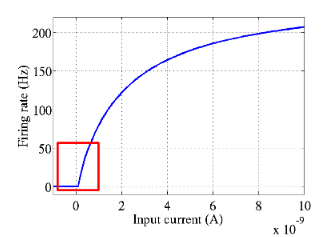
\includegraphics[width=0.6\textwidth]{biological_activation_function.png}
	\caption[Activation function inspired by biological data]{Activation function inspired by biological data\footnotemark}
	\label{fig:biological_activation_function}
\end{figure}
\footnotetext{Taken from \cite{dsrnn}, p. 3}


Another property of the \ac{ReLU}, which makes it biologically more plausible, is the fact that using the \ac{ReLU} as activation function leads to neural networks which tend to be sparse. Sparse neural networks have only few connections or, equivalently, a lot of connections with a weight of zero. These networks are closer to natural neural networks, some of which appear to have only 1\% to 4\% of their neurons activated. On the one hand, sparse neural networks work well on naturally sparse data, on the other hand, a too sparse network may lose a lot of its modeling capability.\\
Being biologically plausible is not necessarily essential to construct a well performing machine learning model. However, in \cite{dsrnn} several comparisons between a network with the \ac{ReLU} as activation function and other models have shown that the \ac{ReLU} network performs better than the other models or is at least competitive. The \acp{CNN} used in this thesis often use combinations of the sigmoidal activation function and the \ac{ReLU}.

\subsection{Feed-forward Neural Networks}
\label{subsec:feed_forward_neural_networks}

The most common \acp{ANN} are still feed-forward neural networks. The neurons in a feed-forward neural network are usually organized in consecutive layers, which propagate the information in only one direction through the network. Figure \ref{fig:ffnn} shows a fully connected feed-forward network with one input layer, one output layer and two layers in between, which are called hidden layers.
\begin{figure}[htbp]
	\centering
	\begin{tikzpicture}[scale=1,every path/.style={>=latex}]
		%draw text nodes
		\node at (0,4.4) {Input Layer};
		\node at (9,4.9) {Output Layer};
		\node at (4.5,5.2) {Hidden Layers};
		% draw first layer
		\foreach \x in {1,...,3}
		{
			\node (n0\x) at (0, \x) [circle,draw,minimum size=0.5cm] {};
		}
		%draw second layer
		\foreach \x in {0,...,4}
     	{
     		\node (n3\x) at (3, \x) [circle,draw,minimum size=0.5cm] {};
     		% draw connections from layer one to layer two
     		\foreach \n in {1,...,3}
     		{
     			\draw[->] (n0\n) to (n3\x);
     		}
     	}
     	%draw third layer
		\foreach \x in {0,...,5}
     	{
     		\node (n6\x) at (6, \x - 0.5) [circle,draw,minimum size=0.5cm] {};
     		% draw connections from layer two to layer three
     		\foreach \n in {0,...,4}
     		{
     			\draw[->] (n3\n) to (n6\x);
     		}
     	}
     	%draw fourth layer
     	\foreach \x in {1,...,4}
     	{
     		\node (n9\x) at (9, \x - 0.5)  [circle,draw,minimum size=0.5cm] {};
     		% draw connections from layer three to layer four
     		\foreach \n in {0,...,5}
     		{
     			\draw[->] (n6\n) to (n9\x);
     		}
     	}
	\end{tikzpicture}
	\caption{Fully connected feed-forward neural network with two hidden layers}
	\label{fig:ffnn}
\end{figure}


As illustrated by the arrows in figure \ref{fig:ffnn}, the information is passed from the leftmost neurons in the input layer to the first hidden layer, then to the second hidden layer and finally to the output layer on the right. The number of neurons in the input layer has to correspond to the dimensionality of the input space. The number of neurons in the output layer is determined by the number of classes in a classification task or the number of desired outputs in a regression task respectively. Hence, these parameters are clearly defined by the problem and are not part of the model definition process. On the other hand, the number of the neurons in the hidden layers and the number of the hidden layers itself depends on the complexity of the task, which shall be solved by the network. For easily solvable problems only a few neurons may suffice, while difficult tasks can require several hundred or thousand neurons. Figuring out an appropriate network architecture is a task whose difficulty should be not underestimated.\\
The above depicted network is called fully-connected, because each neuron in layer $i$ has a connection to each neuron in layer $i + 1$. Note that there are no connections within one single layer. If there were also connections in the other direction, the network would be a \ac{RNN}. Although there are many interesting problems to which \acp{RNN} could be applied to, \acp{RNN} are much less prominent in Machine Learning, because there are very few well-established training algorithms. For feed-forward networks, however, there exist reliable training algorithms. The most used of them is called Backpropagation. Backpropagation profits from the observation that a feed-forward \ac{ANN} is nothing more than a mathematical function, which fulfills the requirements for being differentiable. While the sigmoidal activation function and the hyperbolic tangent activation function are differentiable, the \ac{ReLU} is a bit problematic, because it is not differentiable at $0$. This problem can be eluded by setting the gradient to $0$ at this position. Since Backpropagation is a minimization method, it is necessary to define an error function which is subject to the minimization process . The formula for a very common error function, the \ac{MSSE}, is given in equation \eqref{eq:msse}.
\label{msse}
\begin{align}
\label{eq:msse}
\operatorname{MSSE} = \frac{1}{N} \cdot \sum_{i}^{N} \left(\hat{y}_i - y_i\right)^2
\end{align}
$N$ is the number of samples, e.g. the number of images used for training an \ac{ANN}. $\hat{y}_i$ is the predicted value for the $i$-th input vector $\V{x}_i$ and $y_i$ the true value, i.e. the label, of the said input. The goal of training an \ac{ANN} is to adapt its weights such that its prediction $\hat{y}_i$ is as close as possible to the true label $y_i$. If the two values are very close, the squared difference $(\hat{y}_i - y_i)^2$ is very small and adds almost nothing to the eventual value of the sum. If the values diverge, their squared difference gets very large and the error function increases quadratically. Thus, the \ac{MSSE} error function punishes large deviations more than small deviations.\\
The value $\hat{y}_i$ is the result of the function which is implemented by the neural network, and therefore depends mainly on the weights. Firstly, Backpropagation calculates the gradient of the error function with respect to the weights for a subset of the input data set by applying the chain rule. Since the gradient always points in the direction of the steepest incline, the weights are adapted by subtracting the gradient multiplied with a certain value, which is called learning rate. The learning rate determines how much influence the chosen subset of input data has on the weight changes. One way to choose the mentioned data subset is to consider all data and adapt the weights after presenting all inputs to the network, i.e. calculating the prediction $\hat{y}_i$ for each input vector $\V{x}_i$. The process of presenting all inputs is called an epoch. This method has the advantage of being relatively robust against noise, because it is averaged out as far as the data allows. The disadvantage is that the weights are learned rather slowly, because a lot of epochs are necessary until the network produces good results. Another method, which is called \acf{SGD}, uses only small batches, i.e. the data is divided in $n$ equally sized subsets, which are subsequently presented to the network. The idea is that the gradient of each batch is an approximation of the true gradient. Since the weights are adapted after each batch, the learning process should be faster. One possible caveat, however, is that outliers have a rather strong influence on the weight changes.\\
With $n_i$ as the number of neurons in layer $i$, there are $n_i \cdot n_{i+1}$ connections between layer $i$ and layer $i+1$. That means that there are many connections whose weights have to be learned during the training phase. Since the training time of such a network can easily take several days, more time-efficient models are desirable.

\subsection{Convolutional Neural Networks}

\acfp{CNN} are a specific kind of \acp{ANN}, which perform very well on image data, because they are able to exploit their two-dimensional structure.

\subsubsection{Convolutional Layer}
\label{subsubsec:convolutionallayer}

The key idea is to replace some of the fully connected layers at the beginning of the network with two-dimensional convolutional layers. A very important property of these layers is that they use only little weight patches, which are called filters, for the whole layer instead of connecting each neuron of one layer with all neurons of the succeeding layer. This way many connections can be omitted, resulting in a shorter training time. Figure \ref{fig:centered_filter} shows how one filter in a convolutional layer functions in general.
\begin{figure}[htbp]
	\centering
	\begin{tikzpicture}[scale=0.9,every path/.style={>=latex}]
		\node (layeri) at (2.5,11) {Layer i};
		\node (layeri) at (9.5,10) {Layer i+1};
     	
     	% draw background for filter
     	\draw[fill=pink] (2.5,2.5) rectangle (5.5,-0.5);
     	
     	% draw rectangle with "*" inside
     	\draw[fill=white] (5.2,2.8) rectangle (5.8,2.2);
     	\node at (5.5,2.5) {$*$};
     	
     	
     	% draw layer 1
     	\foreach \x in {0,...,5}
     	{
     		\foreach \y in {0,...,10}
     		{
     			\node(1-\x-\y) at (\x,\y) [circle,draw,minimum size=0.4cm] {};
     		}
     	}
     	
     	% draw layer 2
     	\foreach \x in {1,...,4}
     	{
     		\foreach \y in {1,...,9}
     		{
     			\node(2-\x-\y) at (\x + 7,\y) [circle,draw,minimum size=0.4cm] {};
     		}
     	}
     	
     	%draw filter
     	\foreach \x in {0,...,2}
     	{
     		\foreach \y in {3,...,5}
     		{
     			\node(f-\x-\y) at (\x - 0.06 + 3,\y - 0.06 - 3) [circle,draw,purple,minimum size=0.4cm] {};
     		}
     	}
     	
     	% draw line from filter to "+" rectangle
     	\draw[->] (5.5,0) to (6.7,0);
     	
     	% draw "+" rectangle
     	\draw[fill=white] (6.7,0.3) rectangle (7.3,-0.3);
     	\node at (7,0) {$+$};
     	
     	% draw line from "+" rectangle to ReLU rectangle
     	\draw[->] (7.3,0) to (8.7,0);
     	
     	% draw ReLU rectangle
     	\draw[fill=white] (8.7,0.3) rectangle (9.3,-0.3);
     	\draw[->,out=0,in=270] (9.3,0) to (2-4-1);
     	\draw[-] (8.82,-0.1) to (9.02,-0.1);
     	\draw[-] (9.02,-0.1) to (9.17,0.1);
	\end{tikzpicture}
	\caption{Functioning of a convolutional layer}
	\label{fig:centered_filter}
\end{figure}

The filter in this example has a size of $3\times 3$ and is emphasized by the nine purple circles and by the light red background. The filter in the illustration is currently centered on the fifth neuron from the left and second from the bottom. The multiplication symbol $*$ in the small rectangle in the top right corner of the filter indicates that the activation value of each neuron, which is covered by the filter, is multiplied with the weight of the filter at the corresponding position. The resulting products are summed up to a single value, which is inserted into the activation function and finally becomes the activation of the neuron in layer $i+1$. This is done not only once, but the filter is centered on each neuron of layer $i$ in order to produce the activations of the neurons in layer $i+1$. Using this method, a drastic reduction of weights is achieved by replacing the $n_i \cdot n_{i+1}$ weights, which would be required for a fully connected \ac{ANN}, with a constant number of weights, which is independent of the number of neurons in the two connected layers. The dimensionality of layer $i+1$ is slightly reduced by $(h - 1) / 2$ neurons in horizontal direction and $(v - 1)/2$ neurons in vertical direction (with $h$ = filter height and $v$ = filter width), because the filter is not centered on the outermost neurons. Edge handling techniques known from digital image processing like wrap-around or zero-padding are usually not used. The strong resemblance of the mathematical concept of convolution with the way how the filter's weights are multiplied with the activation values of the neurons is the origin of the name Convolutional Neural Network.

\subsubsection{Maps}
\label{subsubsec:maps}

Contrary to what has been suggested so far, most layers in a \ac{CNN} do not consist of only one two-dimensional array but several ones, which are called maps. A convolutional layer takes all the maps of its preceding layer as input and produces a certain amount of output maps. Figure \ref{fig:cnn_maps} illustrates in detail how such a layer works. The following lines are inspired by the explanations in \cite{gtsrb}.
\begin{figure}[htbp]
	\centering
	\begin{tikzpicture}[xscale=0.9,yscale=0.79,every path/.style={>=latex}]
		% draw input maps		
		\node (IM1) at (2,11.) [draw,rectangle,minimum width=6cm,minimum height=1.7cm] {Input map 1};
		\node (IM2) at (12,11.) [draw,rectangle,minimum width=6cm,minimum height=1.7cm] {Input map 2};
		
		% draw filters
		\node (F11) at (0,7.5) [draw,rectangle,minimum size=1cm] {$F_{11}$};
		\node (F12) at (2,7.5) [draw,rectangle,minimum size=1cm] {$F_{12}$};
		
		\node (F21) at (6,7.5) [draw,rectangle,minimum size=1cm] {$F_{21}$};
		\node (F22) at (8,7.5) [draw,rectangle,minimum size=1cm] {$F_{22}$};

		\node (F31) at (12,7.5) [draw,rectangle,minimum size=1cm] {$F_{31}$};
		\node (F32) at (14,7.5) [draw,rectangle,minimum size=1cm] {$F_{32}$};
		
		% draw lines from input maps to filters
		\draw[->] (IM1.south) to (F11.north);
		\draw[->] (IM2.south) to (F12.north);
		\draw[->] (IM1.south) to (F21.north);
		\draw[->] (IM2.south) to (F22.north);
		\draw[->] (IM1.south) to (F31.north);
		\draw[->] (IM2.south) to (F32.north);
		
		% draw convolution symbols on the filters
		\node[draw,rectangle,fill=white,above right=-0.4cm of F11] {$*$};
		\node[draw,rectangle,fill=white,above left=-0.4cm of F12] {$*$};
		\node[draw,rectangle,fill=white,above right=-0.4cm of F21] {$*$};
		\node[draw,rectangle,fill=white,above left=-0.4cm of F22] {$*$};
		\node[draw,rectangle,fill=white,above right=-0.4cm of F31] {$*$};
		\node[draw,rectangle,fill=white,above left=-0.4cm of F32] {$*$};
		
		% draw output maps
		\node (OM1) at (1,2.5) [draw,rectangle,minimum width=4cm,minimum height=1.5cm] {Output map 1};
		\node (OM2) at (7,2.5) [draw,rectangle,minimum width=4cm,minimum height=1.5cm] {Output map 2};
		\node (OM3) at (13,2.5) [draw,rectangle,minimum width=4cm,minimum height=1.5cm] {Output map 3};
		
		% draw + signs
		\node (P1) at (1,5.6) [draw,rectangle,minimum size=0.5cm] {+};
		\node (P2) at (7,5.6) [draw,rectangle,minimum size=0.5cm] {+};
		\node (P3) at (13,5.6) [draw,rectangle,minimum size=0.5cm] {+};
		
		% draw lines from filters to + signs
		\draw[->] (F11.south) to (P1.north);
		\draw[->] (F12.south) to (P1.north);
		\draw[->] (F21.south) to (P2.north);
		\draw[->] (F22.south) to (P2.north);
		\draw[->] (F31.south) to (P3.north);
		\draw[->] (F32.south) to (P3.north);

		% draw biases
		\node[draw,rectangle,left=of P1] (b1) {$b_1$};
		\node[draw,rectangle,left=of P2] (b2) {$b_2$};
		\node[draw,rectangle,left=of P3] (b3) {$b_3$};

		% draw lines from biases to + signs
		\draw[->] (b1) to (P1);
		\draw[->] (b2) to (P2);
		\draw[->] (b3) to (P3);

		% draw activation functions
		\node (A1) at (1,4.4) [draw,rectangle,minimum size=0.5cm] {};
     	\draw[-] (0.82,4.3) to (1.02,4.3) to (1.17,4.5);
		\node (A2) at (7,4.4) [draw,rectangle,minimum size=0.5cm] {};
     	\draw[-] (6.82,4.3) to (7.02,4.3) to (7.17,4.5);
		\node (A3) at (13,4.4) [draw,rectangle,minimum size=0.5cm] {};
     	\draw[-] (12.82,4.3) to (13.02,4.3) to (13.17,4.5);
		
		% draw lines from + signs to activation functions
		\draw[->] (P1) to (A1);
		\draw[->] (P2) to (A2);
		\draw[->] (P3) to (A3);

		% draw lines from activation functions to output maps
		\draw[->] (A1) to (OM1);
		\draw[->] (A2) to (OM2);
		\draw[->] (A3) to (OM3);
	\end{tikzpicture}
	\caption{How maps are organized in a convolutional layer}
	\label{fig:cnn_maps}
\end{figure}


While the very first layer of a \ac{CNN} often works on exactly three maps, each of which containing the information of one of the three color channels of an \ac{RGB} image, the convolutional layer used in the example network depicted in figure \ref{fig:cnn_maps} has only two input maps for display reasons. The number of the output maps can be chosen arbitrarily, independent of the number of the input maps. The number of the filters, on the other hand, is determined by the product of the number of the input maps and the number of the desired output maps. Hence, the network given in the illustration has exactly $2 \cdot 3 = 6$ filters. The formula for output map $O_j$ is given in equation \eqref{eq:output_map} with $N$ as number of input maps and $I_i$ as $i$-th input map.
\begin{align}
\label{eq:output_map}
O_j = f \left( \sum_i^{N} I_i * F_{ji} + b_j \right)
\end{align}
In order to calculate the output map $O_j$, each input map $I_i$ is convolved with a corresponding filter $F_{ji}$ as described above around figure \ref{fig:centered_filter}. This part is indicated by $I_i * F_{ji}$ in the formula. Thus, the number of filters needed to calculate one single output map is equal to the number of given input maps $N$. All the resulting outputs of the convolutions are summed up to one single two-dimensional array. Subsequently a scalar bias value $b_j$ is added to each element of the current intermediate result. Before this array finally becomes the output map $O_j$, an activation function like the \ac{ReLU} is applied to each neuron.\\
Since the total number of filters in a convolutional layer equals $N \cdot J$ (with $J$ as the number of output maps) and since in general all filters used in a single convolutional layer have the same dimensionality $h \times v$, the total number of weights $\abs{W}$ is computed as shown in equation \eqref{eq:total_number_of_weights}.
\begin{align}
\label{eq:total_number_of_weights}
\abs{W} = N \cdot J \cdot h \cdot v
\end{align}
To determine the total number of free parameters in a convolutional layer, the number of bias values, which corresponds to the number of output maps $J$, has to be added to the number of the weights. Hence, a convolutional layer with five input maps, eight output maps and filters of size $3\times 3$ has $5 \cdot 8 \cdot 3 \cdot 3 +  8 = 368$ trainable parameters in total.

\subsubsection{Max Pooling Layer}
\label{subsubsec:maxpoolinglayer}

Next to the convolutional layer there is another layer, which is normally part of a \ac{CNN}, namely the max pooling layer. This sort of layer is used to increase the translation invariance of the network by combining a patch of neurons in an input map to only one neuron in an output map. This is done by choosing the maximum activation of the contemplated neurons as output. It is very common to use a $2\times 2$ patch, but also larger patches are possible. The considered neuron patches in the input map may overlap, but usually only distinct patches are regarded. Figure \ref{fig:max_pooling} illustrates this concept for a single max pooling operation on a batch of four neurons without overlap.
\begin{figure}[htbp]
	\centering
	\begin{tikzpicture}[scale=0.85,every path/.style={>=latex}]
		\node (layeri) at (2.5,8) {map in layer i};
		\node (layeri) at (9,5.5) {map in layer i+1};
	
     	% draw background for max pooling
     	\draw[fill=pink] (3.5,-0.5) rectangle (5.5,1.5);
     	
     	% draw left layer
     	\foreach \x in {0,...,5}
     	{
     		\foreach \y in {0,...,7}
     		{
     			\node(1-\x-\y) at (\x,\y) [circle,draw,minimum size=0.4cm] {};
     		}
     	}
     	
     	% draw right layer
     	\foreach \x in {0,...,2}
     	{
     		\foreach \y in {0,...,3}
     		{
     			\node(2-\x-\y) at (\x + 8,\y + 1.5) [circle,draw,minimum size=0.4cm] {};
     		}
     	}
     	
     	% draw "+" rectangle
     	\node (max) at (8.5,0.5) [draw,rectangle] {max};
     	
     	% draw line from red rectangle to max
     	\draw[->] (5.5,0.5) to (max);
     	
     	% draw line from max to corresponding neuron in layer i+1
     	\draw[->,out=0,in=270] (max) to (2-2-0);
	\end{tikzpicture}
	\caption{Max Pooling layer}
	\label{fig:max_pooling}
\end{figure}

As depicted in the figure, max pooling drastically decreases the number of neurons by a factor $h$ in horizontal direction and a factor $v$ in vertical direction, given a max pooling patch size of $h\times v$ and no overlap. In contrast to convolutional layers, a max pooling layer keeps the number of maps constant, neither increasing nor decreasing it. Thus, a max pooling layer can only be used for complexity reductions.\\
While the early layers in the network respond to basic features like edges and corners, the later layers in the network, which survey a relatively large area of the image because of the max pooling operation, respond to more complex compound features without having knowledge of the precise locations of all their contributing individual parts. This behavior is desirable particularly for classification tasks, because it is often not necessary to know in detail where the features are located in the image. In regression tasks, however, precise knowledge about the features' position can be very valuable, so the use of max pooling should be left out or at least be limited to a certain degree.\\
Most \acp{CNN} use convolutional layers and max pooling layers alternately, producing more and more high-level feature extractors with increasing depth of the network. After the convolutional and max pooling layers, a small number of fully connected layers follows to connect the responses of the high-level feature extractors logically in order to produce reasonable predictions. The first fully connected layer has one connection to each neuron of each map of the last preceding layer. Since \acp{CNN} often possess very many consecutive layers, the network becomes very deep. This is where the recently often used terms \q{Deep Learning} and \q{Deep Convolutional Network} originate from. The layers introduced in this subsection are important components of the CNNs which are used within this thesis to construct as good an estimator as possible for facial landmarks in images of human faces.
\newpage

%%%%%%%%%%%%%%%%%%%%%%%%%%%%%%%%%%%%%%%%%%%%%%%%%%%%%%%%%%%%%%%%%%%%%%%%%%%%%%%%%%%%%%%%%%%%%%%%%%%%%%%%%
%%%%%%%%%%%%%%%%%%%%%%%%%%%%%%%%%%%%%%%%%%%%%%%%%%%%%%%%%%%%%%%%%%%%%%%%%%%%%%%%%%%%%%%%%%%%%%%%%%%%%%%%%
%									DATA CHAPTER BEGINS HERE											%
%%%%%%%%%%%%%%%%%%%%%%%%%%%%%%%%%%%%%%%%%%%%%%%%%%%%%%%%%%%%%%%%%%%%%%%%%%%%%%%%%%%%%%%%%%%%%%%%%%%%%%%%%
%%%%%%%%%%%%%%%%%%%%%%%%%%%%%%%%%%%%%%%%%%%%%%%%%%%%%%%%%%%%%%%%%%%%%%%%%%%%%%%%%%%%%%%%%%%%%%%%%%%%%%%%%

\section{Data}
\label{sec:data}

Training and testing a \ac{CNN} requires an appropriate data set with a sufficiently large number of training and test examples. Daniel Nouri uses the data set from the \emph{Facial Keypoints Detection} challenge on the machine learning website Kaggle (cf. \cite{kaggle}) in his inspiring tutorial \emph{Using convolutional neural nets to detect facial keypoints} \cite{nouri-tutorial}. This dataset provides a reasonable amount of landmarks, however, it does not provide all landmarks for all faces. To avoid too much data organization overhead the \ac{MUCT} data set taken from \cite{muct} was used instead, which exhibits a simpler data structure while providing the same types of landmarks as the Kaggle data set, plus a few extra ones.

\subsection{Kaggle}

Since the first experiments done in the scope of this thesis were inspired by the tutorial by Daniel Nouri mentioned above, the initial plan was to work with the same data set, which was used there. The data set used in the tutorial is taken from the \emph{Facial Keypoints Detection} challenge on Kaggle and contains 7,049 training images as well as 1,783 test images with a resolution of $96 \times 96$ pixels. All images are provided as gray value images within the range $[0,255]$.\\
There are 15 different landmarks (called keypoints on Kaggle), each of which consists of two scalar values $(x,y)$, which represent the horizontal and vertical position of the corresponding feature in the image. The 15 landmarks are:
\vspace{-0.2cm}
\begin{multicols}{2}
	\begin{itemize}[itemsep=-2ex]
		\item Left eye center
		\item Right eye center
		\item Left eye inner corner
		\item Left eye outer corner
		\item Right eye inner corner
		\item Right eye outer corner
		\item Left eyebrow inner end
		\item Left eyebrow outer end
	\end{itemize}
\columnbreak
	\begin{itemize}[itemsep=-2ex]
		\item Right eyebrow inner end
		\item Right eyebrow outer end
		\item Nose tip
		\item Mouth left corner
		\item Mouth right corner
		\item Mouth center top lip
		\item Mouth center bottom lip
	\end{itemize}
	\vphantom{}
\end{multicols}
\vspace{-0.5cm}
One difficulty of this data set is that not all landmarks exist for all images. In fact, for virtually each landmark, there exists a different set of images, which contain the landmark. This leads to problems, because a \ac{CNN} expects a fixed number of inputs and produces a fixed number of outputs. There are several ways to deal with this problem. One of them is to train a separate predictor for each landmark with all images, which contain information about the regarded landmark. The predictors could then be merged in order to produce values for all landmarks on the test images. Another way could be to predict always all landmarks but to modify the error function such that outputs, which belong to nonexistent landmarks, are not considered. To avoid these problems and because of the rather small image resolution of $96 \times 96$, another data set with a larger image resolution was used.

\subsection{MUCT Face Database}

The \acf{MUCT} face database was created by Stephen Milborrow, John Morkel and Fred Nicolls in December 2008 at the University Of Cape Town (cf. \cite{muct}). It contains 3755 faces with 76 manually set landmarks, including all Kaggle landmarks presented above. As shown in figure \ref{fig:muctfaces}, it provides a broad spectrum of faces from people of different age, gender and ethnicity. Furthermore, many different lighting settings have been used in order to increase the diversity of the pictures.

\begin{figure}[htbp]
	\centering
	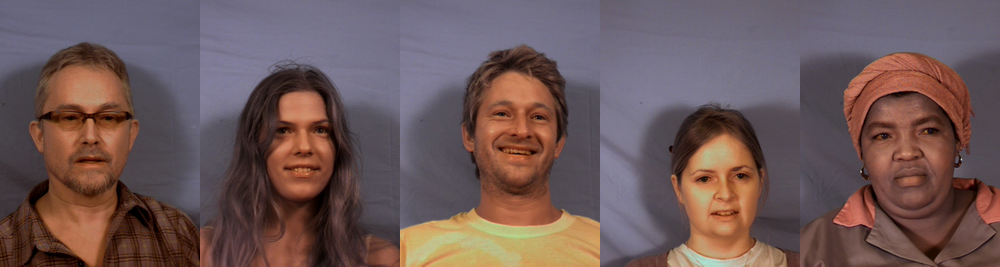
\includegraphics[width=\textwidth]{muct_faces.png}
	\caption{Five faces from the MUCT face database}
	\label{fig:muctfaces}
\end{figure}

Since images in real applications are often not taken from a perfectly frontal perspective on the face, the creators of the data set provide images taken from five different angles, which are shown in figure \ref{fig:muctangles}. Disregarding some negligible software-induced delays, all five images were taken simultaneously in order to guarantee that the person does not move between two photo shots. Whereas two of the images show the right side of the person's face, images of the left side were not taken, because approximations of these images can be easily obtained by mirroring.

\begin{figure}[htbp]
	\centering
	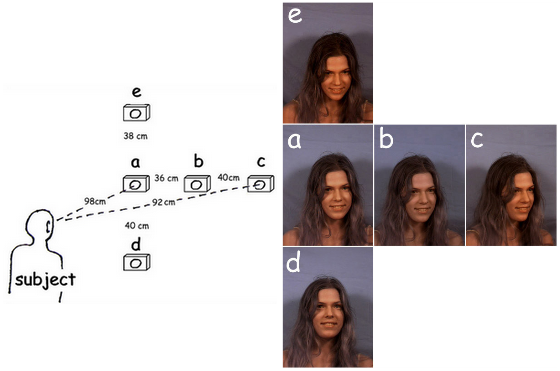
\includegraphics[width=0.77\textwidth]{muct_perspectives.png}
	\caption[MUCT different derspectives]{MUCT different perspectives\footnotemark}
	\label{fig:muctangles}
\end{figure}
\footnotetext{Both illustrations were taken from the \cite{muct} paper}

There is only one real disadvantage of the \ac{MUCT} data set compared to the Kaggle data set, namely the smaller total number of images -- 3755 on \ac{MUCT} instead of 8832 on Kaggle. Apart from that, using the \ac{MUCT} data set has a lot of advantages. The first one is the larger resolution: the \ac{MUCT} images are made available in a resolution of $480 \times 640$ pixels, whereas the Kaggle images have a resolution of only $96 \times 96$ pixels. Even if the full resolution may not be used due to execution time and memory space restrictions, larger resolutions than $96 \times 96$ allow for a model which works more precisely with regard to rather subtle or fine landmarks. Another advantage is the accessibility of color information, which may be useful to produce reasonable predictions at the expense of a longer program execution time.\\
Another expedient property of the \ac{MUCT} data set is its well-structuredness. The file names contain all relevant information about the images, because all of them follow the pattern \texttt{i\{personID\}\{lighting setting\}\{camera view\}-\{gender\}\{(no) glasses\}}. The first \texttt{i}mage of the data set has the file name \texttt{i000qa-fn.jpg}, so the person has the ID \texttt{000}, lighting setting \texttt{q} was used, the photo was shot from angle \texttt{a}, the person is \texttt{f}emale and does \texttt{n}ot wear glasses.\\
This naming scheme is very comfortable, because selecting a certain subset of the images can be achieved by checking their filename for a specific character at the position corresponding to the chosen criterion. This is important, because the \ac{MUCT} data set does not provide all landmarks for all images either, but it does so in a much more organized and transparent way. As pointed out in \cite{muct}, it occurs only for the camera views \texttt{b} and \texttt{c} that some landmarks may not be given, because some of them are not visible due to the perspective on the face. For example the end of a person's left eyebrow is often not visible.\\
Since \acp{ANN} usually require a fixed input size and a fixed output size, all images taken from camera view \texttt{b} and \texttt{c} were omitted and not used at all. For that reason the total number of images shrinks to 2257. These images were divided randomly in 1,752 training images and 502 test images by declaring 20\% of the persons as test persons. No person was assigned to both training set and test, because this way it is easier to measure the generalization capability of the network. Hence, the test images presented to the network always showed persons unknown to the network.

\subsection{Image Preprocessing}
\label{subsec:image_preprocessing}

Before the images are passed to the \ac{CNN} as input, many reasonable preprocessing operations can be applied. On the one hand, the data had to be modified before the whole training process such that training time does not become too long and furthermore that not too much memory space is required. On the other hand, it is reasonable to increase the amount of training data artificially in order to increase the network's generalization ability by distorting the training images a little bit before each epoch.

\subsubsection{Pre-Training Operations}

There are some operations which for several reasons are applied to the training images before the training process itself starts. An important operation is the downscaling of the images, because images with a large resolution like $480\times 640$ pixels cause very long training times. Therefore it is necessary to discard a lot of the information by rescaling the images to resolutions like $96\times 128$ or $120\times 160$ pixels.\\
Another possibility to reduce the training time and the memory demand is to dismiss the color information by transforming the \ac{RGB} images to gray-value images. Since the number of the input maps of the first layer of the \ac{CNN} shrinks from 3 to 1, the network can be trained faster. Additionally the information passed to the network can be increased by using larger resolutions for the input images, because gray-value images do not require as much memory space as \ac{RGB} images. The experiments will show whether the color information or the larger resolution is more valuable.\\
The \ac{PIL} provides many useful image transformation methods. One of them is the \texttt{PIL.ImageOps autocontrast} method, which maximizes the contrast in the image by mapping the darkest pixel of the image to $0$, the lightest pixel to $255$ and all pixels in between to values within the interval from 0 to 255. The goal of applying this method is to simplify the learning task of the network by using the whole possible range of gray-values. This way the network does not have to try to extract information from a much smaller gray-value range than necessary, allowing for less sophisticated weights and therefore ideally for less epochs of training. Figure \ref{fig:autocontrast} shows the difference between an unmodified gray-value image from the \ac{MUCT} data set and its counterpart with maximal contrast.

\begin{figure}[htbp]
	\centering
	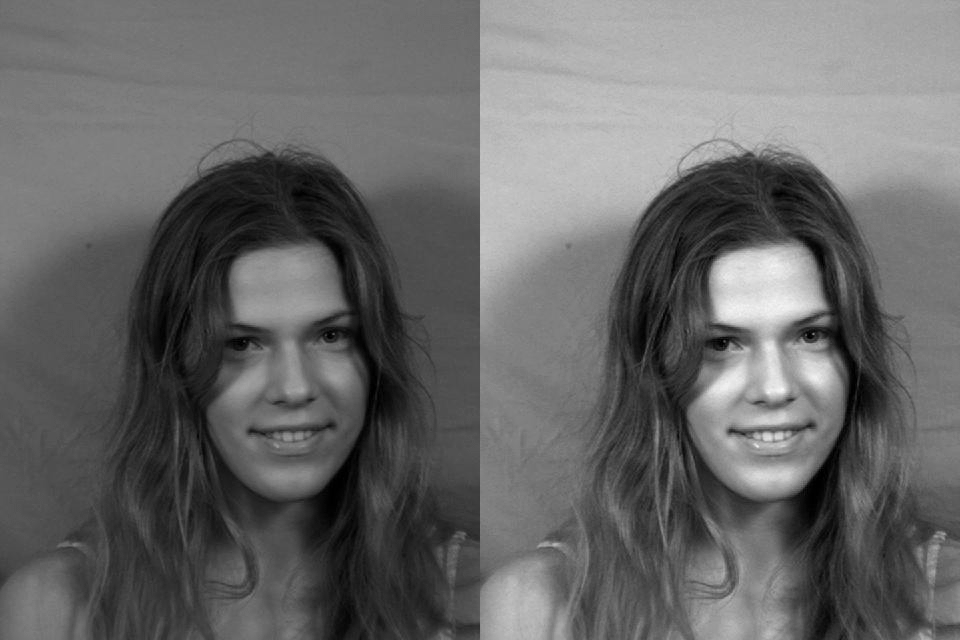
\includegraphics[width=0.5\textwidth]{gray_autocontrast.png}
	\caption{Gray-value (left) and Autocontrast (right)}
	\label{fig:autocontrast}
\end{figure}

After applying the \texttt{autocontrast} method, the gray-values of the image are normalized to the interval $[-1,1]$. The individual coordinates of the labels, however, are normalized to the interval $[0,1]$. Since the activation functions used in the network are zero-centered (sigmoidal function) or change their behavior at 0 (\ac{ReLU}) and since the weights of the layers are usually initialized around 0, it is reasonable to prevent the activation function from saturating by rescaling the gray-values such that they are in the same range.

\subsubsection{On-Line Distortions}

One frequent problem of machine learning is the limited amount of training data. In order to enlarge the distribution from which the training examples are drawn and therefore to increase the generalization ability of the network, it is reasonable to produce more training examples by slightly distorting the already existing ones. Fortunately, there are many operations which can be applied to images without changing them too much. The three operations, which are applied to the images in this thesis, are translation, scaling and rotation. Throughout the whole training process these three operations are applied to each original training image before each epoch. Hence, the network sees slightly different versions of the original training images in every epoch, so that it learns a lot of possible postures of the head, even though the heads are still always from the same persons. A way to avoid that both the original images and all distorted images for the current epoch have to be kept in the memory is to produce the distorted images batch-wise, i.e. a small amount of images is created and passed to the network repeatedly. The used batches can be deleted immediately after having been used.\\
The first operation which is applied to the image, is a horizontal and a vertical shift. The exact number of pixels by which an image is shifted is drawn randomly from a uniform distribution within the interval $[-0.1w, 0.1w]$ in horizontal direction and $[-0.1h, 0.1h]$ in vertical direction with $w$ as width of the image and $h$ as height of the image. Both translations are executed independently from each other and each image is shifted by an individual number of pixels. While the image area that is shifted out of the allowed region is discarded, the pixels which become free after the translation are filled with the content of the closest pixel of the shifted image. The purpose of this operation is to increase the translation invariance of the network. Figure \ref{fig:autocontrast_shifted} shows the image from figure \myref{fig:autocontrast} shifted to the right by 10\% and down by 7\% of the image's width and height respectively.

\begin{figure}[htbp]
	\centering
	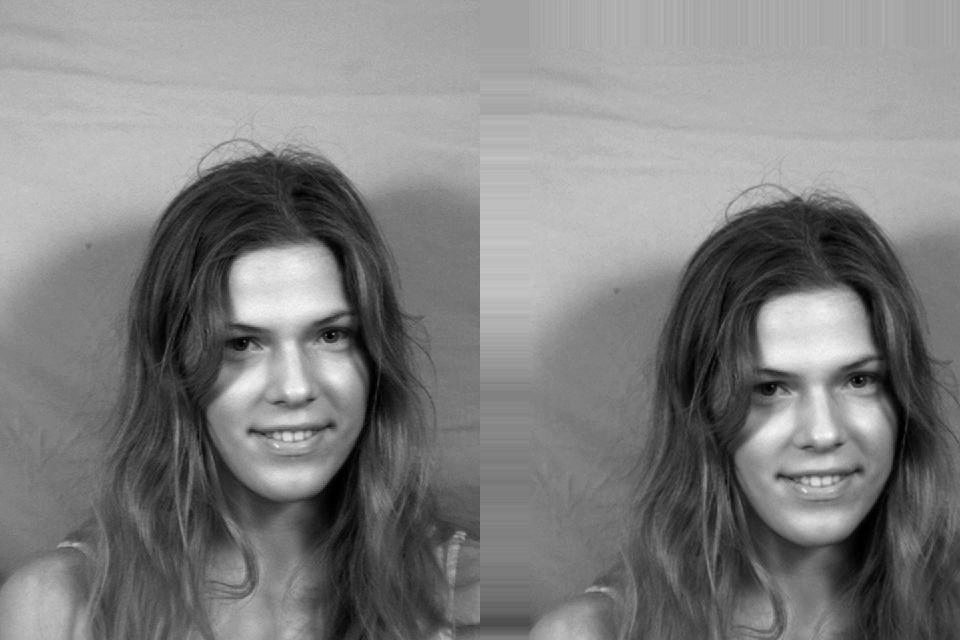
\includegraphics[width=0.5\textwidth]{autcontrast_shifted.png}
	\caption{Contrast enhanced (left) and Shifted (right)}
	\label{fig:autocontrast_shifted}
\end{figure}

After the translation a clockwise rotation by a degree drawn randomly for each image from the interval $[-5,5]$ follows. The corners of the image, which are rotated out of the allowed region, are discarded and the free pixels are filled with the value of the closest pixel of the rotated image. By rotating the images, the network is trained to deal images, which show persons with oblique head postures. Figure \ref{fig:shifted_rotated} shows the shifted image rotated anti-clockwise by 5\%.

\begin{figure}[htbp]
	\centering
	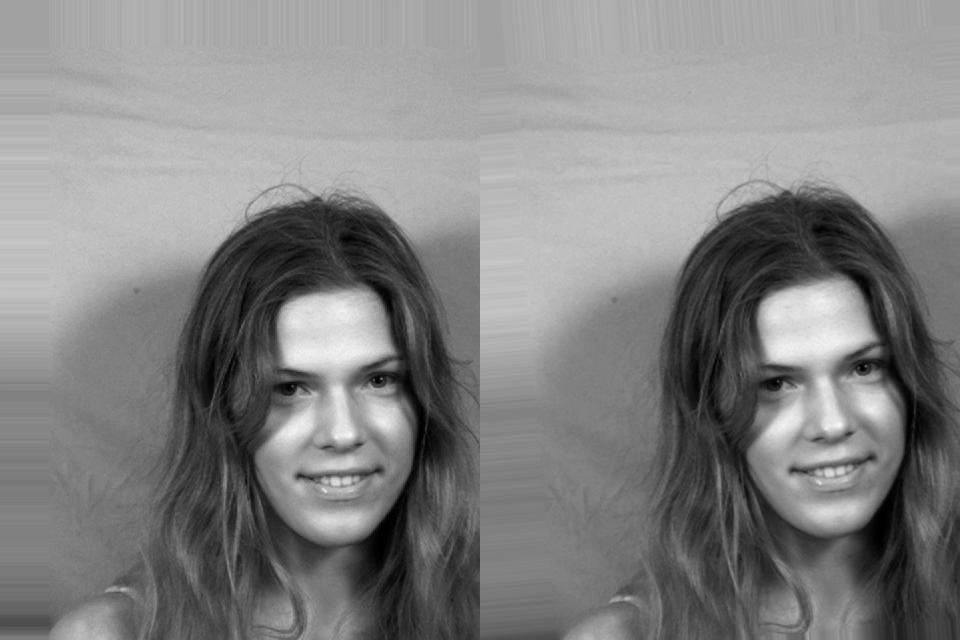
\includegraphics[width=0.5\textwidth]{shifted_rotated.png}
	\caption{Shifted (left) and Rotated (right)}
	\label{fig:shifted_rotated}
\end{figure}

Lastly, each image is scaled individually by a randomly drawn factor from the interval $[-0.9,1.1]$. If the image is enlarged all four borders are cut such that the images assumes the correct resolution. If the image is downsized, it is centered in the new image and the borders are filled with the color value of the closest pixel of the scaled image. The goal of rescaling the images is to allow different head sizes and distances of the persons from the camera. Figure \ref{fig:rotated_scaled} shows the rotated image enlarged by an unrealistically large factor of $1.2$, which was chosen in order to achieve a better visualization.

\begin{figure}[htbp]
	\centering
	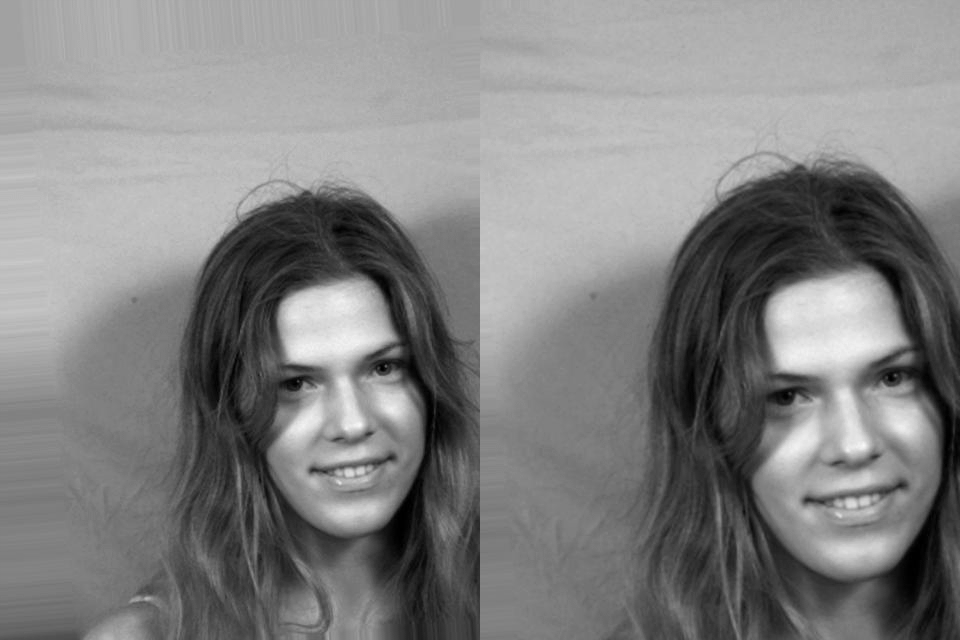
\includegraphics[width=0.5\textwidth]{rotated_scaled.png}
	\caption{Rotated (left) and Scaled (right)}
	\label{fig:rotated_scaled}
\end{figure}

\newpage

%%%%%%%%%%%%%%%%%%%%%%%%%%%%%%%%%%%%%%%%%%%%%%%%%%%%%%%%%%%%%%%%%%%%%%%%%%%%%%%%%%%%%%%%%%%%%%%%%%%%%%%%%
%%%%%%%%%%%%%%%%%%%%%%%%%%%%%%%%%%%%%%%%%%%%%%%%%%%%%%%%%%%%%%%%%%%%%%%%%%%%%%%%%%%%%%%%%%%%%%%%%%%%%%%%%
%								NETWORK ARCHITECTURES CHAPTER BEGINS HERE								%
%%%%%%%%%%%%%%%%%%%%%%%%%%%%%%%%%%%%%%%%%%%%%%%%%%%%%%%%%%%%%%%%%%%%%%%%%%%%%%%%%%%%%%%%%%%%%%%%%%%%%%%%%
%%%%%%%%%%%%%%%%%%%%%%%%%%%%%%%%%%%%%%%%%%%%%%%%%%%%%%%%%%%%%%%%%%%%%%%%%%%%%%%%%%%%%%%%%%%%%%%%%%%%%%%%%

\section{Network Architectures}
\label{sec:networkarchitectures}

Before a \ac{CNN} can be trained to estimate the positions of the landmarks, many decisions have to be made and a lot of parameters have to be set. On the one hand, there are fundamental decisions, which already by themselves have a considerable influence on the success or the failure of the learning process, comprising an appropriate optimization method, a suitable error function, an adequate initialization of the network's weights and the overall structure of the \ac{CNN} like the number, types and sizes of the layers. The optimization method will be the same for all investigated network configurations, namely the \ac{SGD}, which was already described in chapter \myref{subsec:feed_forward_neural_networks}. The error function will the \ac{MSSE} as described in this chapter's second subsection. The weights of the network are initialized according to the method introduced by Xavier Glorot, which facilitates convergence and is described in more detail in the first subsection of this chapter. The number of used layers, their types and their sizes, however, vary from network to network and are adjusted to other parameters like the resolution of the input images.\\
On the other hand, there is large number of parameters, which require fine tuning. Some of these parameters are the learning rate, the size of the batches which are presented successively to the network, the resolution of the input images, the usage or the disuse of the color information and the number of epochs for which the network shall be trained. Each considered network uses a different configuration for these parameters, which are always given for each described network.

\subsection{Initialization}
\label{subsec:glorot_initialization}

Early network configurations using a uniform distribution for initializing the weights of the network have not shown to be very successful. Since it is not trivial to define a reasonable range for the weights, an intelligent initialization of the weights is desirable. Xavier Glorot and Yoshua Bengio introduce such a kind of initialization in their paper \q{Understanding the difficulty of training deep feed-forward neural networks} \cite{glorotinitialization}. The authors of the paper propose the so called \emph{normalized initialization}, which sets the weights according to the formula given in equation \eqref{eq:glorotinitialization}.
\begin{align}
\label{eq:glorotinitialization}
W \sim \mathcal{U} \left[ - \frac{\sqrt{6}}{\sqrt{n_j + n_{j+1}}}, \frac{\sqrt{6}}{\sqrt{n_j + n_{j+1}}} \right]
\end{align}
$\mathcal{U}[a,b]$ is the uniform distribution in the interval from $a$ to $b$, $W$ is the weight matrix of layer $j$ and $n_i$ is the number of neurons found in layer $i$. The bias values were all set to $0$. According to the formula for the weights, the maximal absolute value of the weights between two layers is large if both layers consist of rather few neurons and vice versa.
The advantages of this initialization method are that it helps to avoid the saturation of the activation functions and that it keeps the variances of the activations and the variances of the back-propagated gradients approximately equal in all layers. This way alterations of the weights effectuated by the back-propagation do not vanish and have an actual influence on the optimization process. Next to the uniform distribution there is another initialization method often called Glorot normal initialization, which uses a normal distribution instead of a uniform distribution. It provides the same benefits as the normalized initialization but turns out to work slightly better on the problem given in this thesis than the variant with the uniform distribution. The formula is given in equation \eqref{eq:glorotinitializationnormal}. The second parameter defines the variance of the Gaussian.
\begin{align}
\label{eq:glorotinitializationnormal}
W \sim \mathcal{N} \left(0, \frac{2}{n_j + n_{j+1}} \right)
\end{align}
Even if the considerations in the mentioned paper assume the uniform distribution as well as equal sizes for all layers and were verified for dense \acp{ANN} only, they presumably work well also for different layer sizes and other network architectures like \acp{CNN}. This seems to be confirmed by the results observed in this thesis, which became significantly better after exchanging the initialization with a layer size independent uniform distribution with the Glorot normal initialization.\\

\subsection{Error Function}

All examined networks use the \ac{MSSE}, which was already explained in chapter \myref{msse} and whose formula is given in equation \eqref{eq:msse}. However, it is necessary to explain in detail how the error is calculated, because at the first glance there are at least two different theoretical possibilities. The probably most intuitive way to calculate the error is shown in figure \ref{fig:msse_landmarkwise}.
\begin{figure}[htbp]
	\centering
	
	% landmark-wise distance
	\begin{subfigure}[t]{0.5\textwidth}
		\centering
		\begin{tikzpicture}[scale=0.85,every path/.style={>=latex}]
			% draw grid
			\draw (0.5,0.5) grid (8.5,4.5);
		
			% draw nodes
			\node (E_true) at (3,2) [draw,circle,fill=AI-BLUE] {};
			\node (E_pred) at (6,3) [draw,circle,fill=yellow] {};
			\node [below=0cm of E_true] {True Label};
			\node [above=0cm of E_pred] {Prediction};
		
			% draw arrows
			\draw[<->,line width=1.5] (E_true) to (E_pred);
		\end{tikzpicture}
		\caption{Landmark-wise}
		\label{fig:msse_landmarkwise}
	\end{subfigure}
	% coordinate-wise distance
	\begin{subfigure}[t]{0.49\textwidth}
		\centering
		\begin{tikzpicture}[scale=0.85,every path/.style={>=latex}]
			% draw grid
			\draw (0.5,0.5) grid (8.5,4.5);
		
			% draw nodes
			\node (M_true) at (3,2) [draw,circle,fill=AI-BLUE] {};
			\node (M_pred) at (6,3) [draw,circle,fill=yellow] {};
			\node [below=0cm of M_true] {True Label};
			\node [above=0cm of M_pred] {Prediction};

			% draw arrows
			\draw[<->,line width=1.5] (M_true) to (6,2);
			\draw[<->,line width=1.5] (6,2) to (M_pred);
		\end{tikzpicture}
		\caption{Coordinate-wise}
		\label{fig:msse_coordinatewise}
	\end{subfigure}
	
	\caption{Two different distance measures for calculating the \ac{MSSE}}
	\label{fig:msse}
\end{figure}

This landmark-wise method adds up the squared Euclidean distances between the landmarks predicted by the network (yellow) and the true landmarks (blue). In this scenario the network seems to "know" that the $x$-coordinate and the $y$-coordinate of one landmark constitute a unit. A second possibility is shown in figure \ref{fig:msse_coordinatewise}, where the $x$-coordinate and the $y$-coordinate of a landmark are considered as two independent output values. Here both the horizontal and the vertical deviation are calculated and squared separately. Intuitively, the network should not treat a pair containing the two outputs for one landmark's coordinates differently than a pair of two arbitrarily chosen output values. However, the value produced by the error function does not change at all, no matter which way to calculate it may be chosen. This is proven by the equations \eqref{eq:equal_msse_start} - \eqref{eq:equal_msse_end}. Note that $\l_x$ is the difference between the true and the predicted $x$ value of landmark $l$.
\begin{align}
\label{eq:equal_msse_start}
\sum_{l\ \in \text{ Landmarks}} \sqrt{l_x^2 + l_y^2}^2 &= \sum_{c\ \in \text{ Coordinates}} c_x^2 + c_y^2\\
\equiv \hspace{0.3cm} \sqrt{a_x^2 + a_y^2}^2 + \sqrt{b_x^2 + b_y^2}^2 + \sqrt{c_x^2 + c_y^2}^2 &= a_x^2 + a_y^2 + b_x^2 + b_y^2 + c_x^2 + c_y^2\\
\label{eq:equal_msse_end}
\equiv \hspace{1.95cm} a_x^2 + a_y^2 + b_x^2 + b_y^2 + c_x^2 + c_y^2 &= a_x^2 + a_y^2 + b_x^2 + b_y^2 + c_x^2 + c_y^2
\end{align}
Hence, both methods are completely equivalent and since the coordinate-wise error function is easier to implement, it was used for all networks in the scope of this thesis.\\
The definition of the error function serves its mathematical and computational purpose, but the resulting error value is not very intuitive for human observers due to the normalization of the labels to the unit interval. The standard way of transforming the error value into a more intuitively comprehensible value is to compute its square root and to multiply it with the resolution of the largest dimension of the training images. The result of this calculation is an approximation of the average distance in pixels of the predicted labels from the true labels.

\subsection{Conventionally Trained CNN}
\label{subsec:conventiallytrainedcnn}

During the initial phase of this thesis many classical \acp{CNN} with various parameter settings have been constructed. While the purpose of this subsection is to describe the general structure of these \acp{CNN} only, the results chapter will give insight to the detailed para\-meter settings for each tested network.\\
Since it is difficult to find a suitable network architecture offhand without further knowledge or intuition, especially the networks in the early stages of this thesis are very similar to those, which were used in Daniel Nouri's tutorial \cite{nouri-tutorial}. Figure \ref{fig:example_cnn} shows a possible example network with two convolutional layers, each of which succeeded by a max pooling layer with a patch size of $2\times 2$. Before specifying the details of the network structure, it must be mentioned that for space saving reasons the depicted number of neurons does not correspond to the actually displayed number of neurons. In addition, the activation functions and biases were omitted for the sake of improved clarity. For the same reason there are only two convolutional layers instead of three like in \cite{nouri-tutorial}.
\begin{figure}[h!]
	\centering
	\begin{tikzpicture}[scale=0.75,every path/.style={>=latex}]%0.635%0.73
		% ========================================================================================= %
		% draw input maps
		\def\limX{0} % x-position of the leftmost input map
		\def\limY{1} % y-position of the leftmost input map
		\node at (\limX - 4, \limY + 1) {\small 3 input maps};
		
		\draw[step=0.1] (\limX,\limY) grid (\limX + 1.5,\limY + 2.0);
		\draw[step=0.1] (\limX + 2,\limY) grid (\limX + 3.5,\limY + 2.0);
		\draw[step=0.1] (\limX + 4,\limY) grid (\limX + 5.5,\limY + 2.0);
		
		% ========================================================================================= %
		% draw first convolutional and max pooling layer
		\def\lflmX{-5} % x-position of the leftmost first layer map
		\def\lflmY{-3} % y-position of the leftmost first layer map
		\node at (\lflmX - 1, \lflmY + 2.7) {\small 96 convolutional filters};
		\node at (\lflmX - 0.5, \lflmY + 0.8) {\small 32 maps};
		\node at (\lflmX - 1, \lflmY - 0.5) {\small 32 max pooling filters};
		\node at (\lflmX - 0.5, \lflmY - 1.5) {\small 32 maps};
		
		\foreach \x in {-1,0,2,3}
		{
			% draw maps of the first convolutional layer
			\draw[step=0.1] (2 * \x - 0.001,\lflmY - 0.001) grid (2* \x + 1.201,\lflmY + 1.6);
			
			% draw filters to the map
			\foreach \i in {0,...,2}
			{
				% draw filter
				\draw[step=0.1] (2 * \x + 0.4 * \i - 0.001,\lflmY + 2.5 - 0.001) grid (2* \x + 0.4 * \i + .301,\lflmY + 2.5 + .301);
				
				% draw connections from input maps to the filters
				\draw[->] (\limX + \i * 2 + 0.75,\limY) to (2 * \x + 0.4 * \i + 0.15,\lflmY + 2.5 + .301);
				
				% draw connections from filter to next map
				\draw[->] (2 * \x + 0.4 * \i + 0.15, \lflmY + 2.5 - 0.001) to (2 * \x + 0.6,\lflmY + 1.6);
			}
		
			% draw max pooling filter
			\draw[step=0.1] (2 * \x + 0.499,\lflmY - .601) grid (2* \x + .701,\lflmY - .399);
			
			% draw connection from first convolutional layer maps to max pooling filters
			\draw[->] (2* \x + 0.6,\lflmY + 1.6) to (2* \x + .6,\lflmY - .399);
			
			% draw first max pooling layer map
			\draw[step=0.1] (2 * \x + 0.199,\lflmY - 2.101) grid (2* \x + 1.001,\lflmY + -1.0);
			
			% draw connection from max pooling filter to max pooling map
			\draw[->] (2 * \x + 0.6,\lflmY - .601) to (2* \x + .6,\lflmY + -1.0);
		}
		
		% draw dots between the filters and the first layer maps
		\node at (\lflmX + 7.7, \lflmY - 1.6) {\ldots};
		\node at (\lflmX + 7.7, \lflmY - 0.5) {\ldots};
		\node at (\lflmX + 7.7, \lflmY + 0.7) {\ldots};
		\node at (\lflmX + 7.7, \lflmY + 2.65) {\ldots};
		
		% ========================================================================================= %
		% draw second convolutional and max pooling layer
		\def\lslmX{-5} % x-position of the leftmost first layer map
		\def\lslmY{-9.5} % y-position of the leftmost first layer map

		\node at (\lslmX - 3, \lslmY + 2.7) {\small 2048 convolutional filters};
		\node at (\lslmX - 2.5, \lslmY + 1.2) {\small 64 maps};
		\node at (\lslmX - 3, \lslmY + 0.1) {\small 64 max pooling filters};
		\node at (\lslmX - 2.5, \lslmY - 1.0) {\small 64 maps};
		
		\foreach \x in {-2,-1,0,2,3,4}
		{
			% draw second convolutional layer maps
			\draw[step=0.1] (2 * \x + 0.299,\lslmY + 0.799) grid (2* \x + 0.901,\lslmY + 1.6);
			
			% draw filters to the map
			\foreach \i in {-1,0,2,3}
			{
				% draw filter
				\draw[step=0.1] (2 * \x + 0.3 * \i + 0.199,\lslmY + 2.5 - 0.001) grid (2* \x + 0.3 * \i + .401,\lslmY + 2.5 + .201);
				
				% draw connections from first max pooling layer maps to the filters
				\draw[->] (2 * \i + 0.6,\lflmY - 2.101) to (2* \x + 0.3 * \i + .3,\lslmY + 2.4 + .301);
				
				% draw connections from filter to next map
				\draw[->] (2 * \x + 0.3 * \i + 0.3, \lslmY + 2.5 - 0.001) to (2 * \x + 0.6,\lslmY + 1.6);
			}
			
			% draw dots between the filters of this map
			\node at (2 * \x + 0.6,\lslmY + 2.6) {\tiny ...};
			
			% draw max pooling filter
			\draw[step=0.1] (2 * \x + 0.499,\lslmY - .001) grid (2* \x + .701,\lslmY + .201);
			
			% draw connection from second convolutional layer maps to max pooling filters
			\draw[->] (2* \x + 0.6,\lslmY + 1.6) to (2* \x + .6,\lslmY + .201);
			
			% draw second max pooling layer map
			\draw[step=0.1] (2 * \x + 0.399,\lslmY - 1.201) grid (2* \x + .801,\lslmY + -0.6);
			
			% draw connection from max pooling filter to max pooling map
			\draw[->] (2 * \x + 0.6,\lslmY + .201) to (2* \x + .6,\lslmY + -0.6);
		}
		
		% draw dots between the filters and the first layer maps
		\node at (\lslmX + 7.7, \lslmY + 0.15) {\ldots};
		\node at (\lslmX + 7.7, \lslmY - 0.9) {\ldots};
		\node at (\lslmX + 7.7, \lslmY + 1.2) {\ldots};
		\node at (\lslmX + 7.7, \lslmY + 2.65) {\ldots};
		
		% ========================================================================================= %
		% draw first fully connected layer
		\def\lffclX{-4} % leftmost x-position of the first fully connected layer
		\def\rffclX{9} % rightmost x-position of the first fully connected layer
		\def\ffclY{-13} % y-position of the first fully connected layer
		\node at (\lffclX - 3,\ffclY) {\small 500 neurons};
		
		\foreach \x in {\lffclX,...,\rffclX}
		{
			\node (n\x) at (\x,\ffclY) [draw,circle,inner sep=0pt,minimum size = 0.2cm] {};
			
			\foreach \a in {-2,-1,0,2,3,4}
			{
				\draw[->] (2 * \a + 0.599,\lslmY - 1.201) to (n\x);
			}
		}
		
		% ========================================================================================= %
		% draw second fully connected layer
		\def\lsfclX{-3} % leftmost x-position of the second fully connected layer
		\def\rsfclX{8} % rightmost x-position of the second fully connected layer
		\def\sfclY{-15.} % y-position of the second fully connected layer
		\node at (\lsfclX - 3,\sfclY) {\small 400 neurons};
		
		\foreach \x in {\lsfclX,...,\rsfclX}
		{
			\node (m\x) at (\x,\sfclY) [draw,circle,inner sep=0pt,minimum size = 0.2cm] {};
			
			\foreach \a in {\lffclX,...,\rffclX}
			{
				\draw[->] (n\a) to (m\x);
			}
		}
		
		% ========================================================================================= %
		% draw output layer
		\def\lolX{1} % leftmost x-position of the output layer
		\def\rolX{3} % rightmost x-position of the output layer
		\def\olY{-17.} % y-position of the output layer
		\node at (\lolX - 5,\olY) {\small 30 output neurons};
		
		\foreach \x in {\lolX,...,\rolX}
		{
			\node (q\x) at (\x + 0.5,\olY) [draw,circle,inner sep=0pt,minimum size = 0.2cm] {};
			
			\foreach \a in {\lsfclX,...,\rsfclX}
			{
				\draw[->] (m\a) to (q\x);
			}
		}
	\end{tikzpicture}
	\caption{A complete example \ac{CNN}}
	\label{fig:example_cnn}
\end{figure}
\\
It is assumed that the network takes \ac{RGB} images, hence there are three input maps, one for each color channel. The first convolutional layer is supposed to produce 32 output maps, hence according to the explanations in chapter \myref{subsubsec:maps} there are 96 filters between the input layer and the first convolutional layer. As indicated in the figure, the resulting 32 output maps of the first convolutional layer are a bit smaller in both dimensions, because the edges of the input maps are not treated. The 32 output maps of the first convolutional layer constitute the input of the first max pooling layer, which reduces the dimensionality of the maps by a factor of 2 in both dimensions. The second convolutional layer generates 64 output maps, thus $32 \cdot 64 = 2048$ filters are necessary to execute the convolution operation. Also these 64 resulting slightly smaller maps are max pooled, yielding 64 significantly smaller maps. After the second max pooling operation, two fully connected layers follow. Each neuron in the 64 output maps of the second max pooling layer has a connection to each neuron in the first fully connected layer. Assuming a resolution of $22\times 30$ in the 64 max pooling maps and 500 neurons in the first fully connected layer, there are $22 \cdot 30 \cdot 64 \cdot 500 = 21.120.000$ connections, which have to be trained. The second fully layer in this example consists of 400 neurons, thus there are $500 \cdot 400 = 200.000$ connections between the two fully connected layers. The last layer of the network is the output layer, which has as many neurons as there exist desired output values. In the landmark estimation task examined in this thesis the number of output neurons equals 30, because the networks were usually trained to predict the $x$-coordinate and the $y$-coordinate of 15 landmarks.\\
Even if the details will be different for each of the actually trained networks, which are presented in the results chapter, this example network should give a visual intuition for the qualitative structure of a \ac{CNN}. In the results chapter there will be detailed information about the used layer types, layer sizes, weight initializations, activation functions, learning rates and every other important parameter.

\subsection{Gabor CNNs}
\label{subsec:gaborcnns}

After training various conventional \acp{CNN} another biologically inspired kind of \ac{CNN} was constructed and tested in several different configurations. In biology there are various kinds of cells involved in the process of vision. The simple cells in the primary visual cortex detect very elementary features like corners and edges and propagate forward their output to the complex cells, which for their part are high-level feature extractors. They receive input from several simple cells and combine them in order to detect more complex features composed of simpler elements. \acp{CNN} behave similarly as the filters of the early layers resemble simple cells and as the filters in the deeper layers can be considered complex cells. So far, all weights of the network were trained during the learning process. The idea of the networks presented in this subsection is to refrain from training the weights of the filters of the first convolutional layer and to replace them with biologically inspired filters, which are known to work well on image data. According to \cite{ebgm} Gabor wavelets are regarded a suitable model of the simple cells, thus, they might be an adequate choice for being set as filters in the first convolutional layer. Before describing in detail the structure of the used networks, it is necessary to introduce the Gabor wavelets mathematically. They were computed according to formula \eqref{eq:gabor_wavelet}, which is taken from \cite{ebgm}.
\begin{align}
\label{eq:gabor_wavelet}
\psi_{\vec{k}}(\vec{x}) = \frac{\vec{k}}{\sigma^2} \cdot \exp\left(-\frac{\vec{k}^2\vec{x}^2}{2\sigma^2}\right) \cdot \left(\exp\left(i\vec{k}\vec{x}\right) - \exp\left(-\frac{\sigma^2}{2}\right)\right)
\end{align}
The formula contains three exponential functions, the first of which is a Gaussian, whose width is defined by $\frac{\sigma}{k}$. Euler's formula states that $\exp(ix) = \cos x + i \sin x$, hence the second exponential makes the whole function complex. Its real part is determined by a cosine-wave and the imaginary part by a sine-wave. Vector $\vec{k}$ in the argument of the exponential function defines the spatial frequency (and therefore the width) and the orientation of the waves. The third exponential function corrects the wavelet such that it has zero mean, while the factor at the beginning of the formula ensures the normalization of the wavelet. An important property of the here defined wavelets is that for a fixed $\sigma$ they are identical versions of each other apart from scaling and rotation, which are defined by $\vec{k}$.\\
Formula \eqref{eq:gabor_wavelet} describes a continuous version of the Gabor wavelets. Since the Gabor wavelets shall be used in a computer model, it is necessary to discretize them. The wavelets themselves are discretized by means of the image resolution, whereas wave vector $\vec{k}$ is calculated for a chosen subset of widths and frequencies as shown in equation \eqref{eq:k}. 
\begin{align}
\label{eq:k}
\vec{k}_{m,l} = k_\text{max} \alpha^{-m} \begin{pmatrix}\cos\left(\frac{\pi l}{L}\right)\\ \sin\left(\frac{\pi l}{L}\right)\end{pmatrix} \quad m = 0, \ldots, M - 1, \quad l = 0, \ldots, L-1
\end{align}
The variable $L$ defines the number of orientations, while the variable $M$ determines the number of frequencies. \cite{ebgm} recommends specific values for each of the variables except for $k_\text{max}$. While $k_\text{max}$ was set to $\frac{\pi}{2}$, the other values were copied from \cite{ebgm}. Hence, all Gabor wavelets created in this thesis use the following parameter configuration: $\alpha = \sqrt{2}$, $\sigma = 2\pi$, $L = 8$ and $M = 5$. Thus, there are eight orientations and five frequencies, yielding 40 filters each with a real part and an imaginary part. Figure \ref{fig:gabor_filters} illustrates the real parts of the 40 resulting filters. Since the imaginary parts are solely slightly phase-shifted but look otherwise  exactly like the real parts, they were omitted in the figure.
\begin{figure}[htbp]
	\centering
	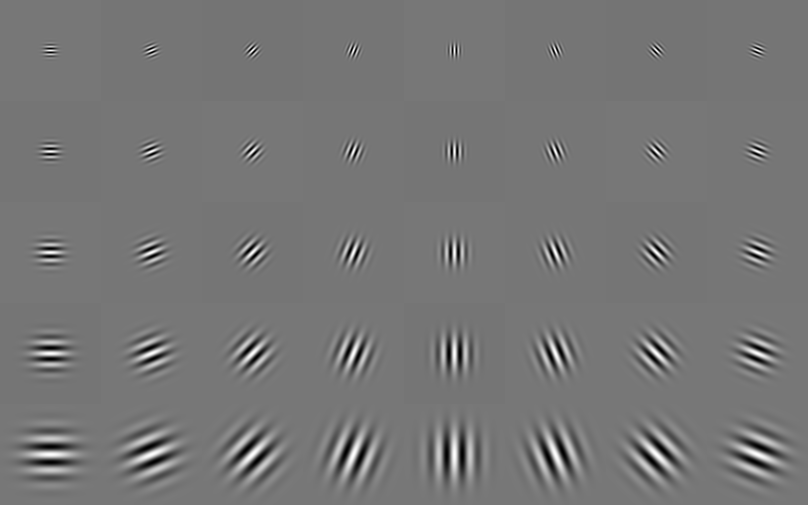
\includegraphics[width=\textwidth]{gabor_filters_normalized_filterwise_real.png}
	\caption{40 gabor filters with 8 different orientations and 5 different widths}
	\label{fig:gabor_filters}
\end{figure}\\
The filters depicted in the figure all have a size of $101 \times 101$. The size of the filters used in the \acp{CNN}, however, was reduced by cutting off the area around the wavelets, which contains only values smaller than $10^{-3}$. Since there are 5 different spatial frequencies, there are also 5 different filter sizes, namely $27 \times 27$ for $M = 0$, $31 \times 31$ for $M = 1$, $39 \times 39$ for $M = 2$, $47 \times 47$ for $M = 3$ and finally $55 \times 55$ for $M = 4$. This has the two advantages of reducing the computation time and avoiding convolutions of the input images with filter values so close to 0 that the results contain almost no information. Figure \ref{fig:gabor_filter_sizes} shows the actually used areas of the filters for $L=0$ and $M \in \{0,\ldots,4\}$. All values, which are not inside the red square, are omitted.
\begin{figure}[htbp]
	\centering
	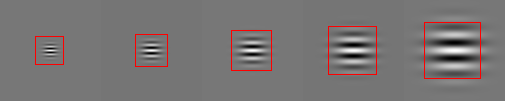
\includegraphics[width=\textwidth]{gabor_filter_sizes.png}
	\caption{The 5 actual filter sizes for $L=0$ and $M \in \{0,\ldots,4\}$}
	\label{fig:gabor_filter_sizes}
\end{figure}

\subsubsection{Gabor Layer}
\label{subsubsec:gaborlayer}

After creating the digital versions of the Gabor wavelets, they have to be incorporated in a \ac{CNN}. It was already mentioned that the filters of the first convolutional layer will be replaced with the Gabor wavelets. However, there are still many open questions about the detailed structure of this first layer, the way how to further process the responses of the wavelets and how to construct the overall structure of the \ac{CNN}. Firstly, the structure of the first convolutional layer, which will be called Gabor layer from now on, will be examined closely. The Gabor layer itself actually consists of two layers, one of them containing the real parts and one of them the imaginary parts of the Gabor filters. The exact number of filters depends on whether color information is used or not. If the network relies on gray-values only, there are exactly 40 real filters and 40 imaginary filters (with $L = 8$ and $M = 5$). Figure \ref{fig:merge_real_imag} illustrates how the Gabor layer is organized.

\begin{figure}[htbp]
	\centering
	\newcommand\sfMergeRealImag{0.9}
	\newcommand\gridnode[5]{
		\node (#1) at (#2 + #4 / 2,#3 + #5 / 2) [minimum width=#4cm * \sfMergeRealImag,minimum height=#5cm * \sfMergeRealImag] {};
		\draw[step=0.1] (#2 - 0.001,#3 - 0.001) grid (#2+#4 + 0.001,#3+#5 + 0.001);	
	}
	\begin{tikzpicture}[scale=\sfMergeRealImag,every path/.style={>=latex}]
		% draw input image
		\gridnode{inputimage}{7.7}{3}{1.5}{2}
	
		% draw background boxes
		\draw[fill=lightgray] (0,1.5) rectangle (8,-0.5);
		\draw[fill=lightgray] (9,1.5) rectangle (17,-0.5);
	
		% draw real filters
		\foreach \x in {0,...,3}
		{
			\gridnode{r\x}{\x * 2 + 0.5}{0}{1}{1}
			\node at (\x * 2 + .5, 1) [draw,fill=white] {$*$};
			\draw[->] (inputimage.south) to (r\x.north);
			\node (ar\x) at (\x * 2 + 1., -1.3) [draw,rectangle,minimum size=0.5cm] {};
			\draw[-] (\x * 2 + 0.85, -1.4) to (\x * 2 + 1.05,-1.4) to (\x * 2 + 1.15, -1.2);
			\draw[->] (r\x.south) to (ar\x.north);
		}
		
		% draw imaginary filters
		\foreach \x in {0,...,3}
		{
			\gridnode{i\x}{\x * 2 + 9.5}{0}{1}{1}
			\node at (\x * 2 + 10.5, 1) [draw,fill=white] {$*$};
			\draw[->] (inputimage.south) to (i\x.north);
			\node (ai\x) at (\x * 2 + 10., -1.3) [draw,rectangle,minimum size=0.5cm] {};
			\draw[-] (\x * 2 + 9.85, -1.4) to (\x * 2 + 10.05,-1.4) to (\x * 2 + 10.15, -1.2);
			\draw[->] (i\x.south) to (ai\x.north);
		}
		
		% draw merge operators
		\foreach \x in {0,...,3}
		{
			\node (m\x) at (\x * 3 + 4,-3.5) [draw,rectangle] {merge op};
			\draw[->] (ar\x.south) to (m\x.north);
			\draw[->] (ai\x.south) to (m\x.north);
		}
		
		% draw output maps
		\foreach \x in {0,...,3}
		{
			\gridnode{o\x}{\x * 3 + 3.4}{-6.6}{1.2}{1.6}
			\draw[->] (m\x.south) to (o\x.north);
		}
		
		% draw text nodes
		\node at (6,4) {Input image};
		\node at (4,2.5) {40 real filters};
		\node at (13.5,2.5) {40 imaginary filters};
		\node at (1.5,-3.5) {Merging};
		\node at (1.55,-6.) {40 output maps};
	\end{tikzpicture}
	\caption{Merging the real and the imaginary filters}
	\label{fig:merge_real_imag}
\end{figure}


The very top of the figure shows the input image, consisting of only one map due to the refusal of the color information. Directly below there are depicted four of the forty real filters on the left and four of the forty imaginary filters on the right. The input map is convolved with each of these 80 filters, resulting in 40 real output maps and 40 imaginary output maps. Then, these 80 output maps are inserted into an activation function like the \ac{ReLU}. Afterwards, the output map of the real filter and the output map of the imaginary filter, which originally belonged to one single Gabor filter, are merged. This process is illustrated by the small rectangles containing the text \q{merge op}. The result of the individual merging operations are 40 output maps, which are going to become the input of a subsequent layer. If the color information is included into the calculation, there are three input maps instead of one, increasing the number of filters from 80 to 240. Since each color channel should be convolved with the same values, each of the 80 filters must be used three times, one time for each color channel. As illustrated by figure \myref{fig:cnn_maps}, the responses of the three filters are added up and inserted into the activation function. Independent of whether the color information is used or not, there exists exactly one bias value for each filter. These values are omitted in figure \ref{fig:merge_real_imag} in order to keep the figure as clearly arranged as possible.\\
The figure only says \q{merge op} instead of describing the exact way how the merging is done, because there are several possibilities to combine the responses of the real and the imaginary filters. Two different operations were realized in the scope of this thesis, namely the absolute value and the phase. Both operations work element-wise, combining the activations of each neuron in the real filter's output and its corresponding neuron in the imaginary filter's output as shown in the equations \eqref{eq:abs} and \eqref{eq:atan2}.
\begin{align}
\label{eq:abs}
a_m &= \sqrt{a_r^2 + a_i^2} = \operatorname{abs}(a_r, a_i)\\
\label{eq:atan2}
a_m &= \operatorname{atan2}(a_i, a_r)
\end{align}
$a_m$ is the activation in the merged map, $a_r$ the real response and $a_i$ the imaginary response. The first method calculates the length of the vector $(a_r,a_i)$ in the complex plane, the second method calculates the angle between the positive half of the $x$-axis (here the imaginary axis) and the point $(a_i,a_r)$ in the complex plane. The absolute value reflects the strength of the response of the filters to the input image, i.e. the resemblance of the filters to the input. The phase, on the other hand, indicates the relative strength of the real response to the imaginary response. If the phase is close to $0$ or $\pi$ (or $0^\circ$ and $180^\circ$) the imaginary response is stronger than the real one. If the phase is close to $\frac{\pi}{2}$ or $\frac{3\pi}{2}$ (or $90^\circ$ or $270^\circ$) the real response is stronger than the imaginary response.\\
Aside from choosing only one of these two methods, it is possible to profit from both approaches by using the absolute value and the phase. This is illustrated in figure \ref{fig:merge_abs_atan2}.
\begin{figure}[htbp]
	\centering
	\newcommand\sfMergeRealImag{0.85}
	\newcommand\gridnode[5]{
		\node (#1) at (#2 + #4 / 2,#3 + #5 / 2) [minimum width=#4cm * \sfMergeRealImag,minimum height=#5cm * \sfMergeRealImag] {};
		\draw[step=0.1] (#2 - 0.001,#3 - 0.001) grid (#2+#4 + 0.001,#3+#5 + 0.001);	
	}
	\begin{tikzpicture}[scale=\sfMergeRealImag,every path/.style={>=latex}]
		% draw input image
		\gridnode{inputimage}{7.7}{3}{1.5}{2}
	
		% draw background boxes
		\draw[fill=lightgray] (0,1.5) rectangle (8,-0.5);
		\draw[fill=lightgray] (9,1.5) rectangle (17,-0.5);
	
		% draw real filters
		\foreach \x in {0,...,3}
		{
			\gridnode{r\x}{\x * 2 + 0.5}{0}{1}{1}
			\node at (\x * 2 + .5, 1) [draw,fill=white] {$*$};
			\draw[->] (inputimage.south) to (r\x.north);
			\node (ar\x) at (\x * 2 + 1., -1.3) [draw,rectangle,minimum size=0.5cm] {};
			\draw[-] (\x * 2 + 0.85, -1.4) to (\x * 2 + 1.05,-1.4) to (\x * 2 + 1.15, -1.2);
			\draw[->] (r\x.south) to (ar\x.north);
		}
		
		% draw imaginary filters
		\foreach \x in {0,...,3}
		{
			\gridnode{i\x}{\x * 2 + 9.5}{0}{1}{1}
			\node at (\x * 2 + 10.5, 1) [draw,fill=white] {$*$};
			\draw[->] (inputimage.south) to (i\x.north);
			\node (ai\x) at (\x * 2 + 10., -1.3) [draw,rectangle,minimum size=0.5cm] {};
			\draw[-] (\x * 2 + 9.85, -1.4) to (\x * 2 + 10.05,-1.4) to (\x * 2 + 10.15, -1.2);
			\draw[->] (i\x.south) to (ai\x.north);
		}
		
		% draw abs operators
		\foreach \x in {0,...,3}
		{
			\node (abs\x) at (\x * 2 + 1,-3.5) [draw,rectangle] {abs};
			\draw[->] (ar\x.south) to (abs\x.north);
			\draw[->] (ai\x.south) to (abs\x.north);
		}
		
		% draw atan2 operators
		\foreach \x in {0,...,3}
		{
			\node (atan2\x) at (\x * 2 + 10,-3.5) [draw,rectangle] {atan2};
			\draw[->] (ar\x.south) to (atan2\x.north);
			\draw[->] (ai\x.south) to (atan2\x.north);
		}
		
		% draw abs output maps
		\foreach \x in {0,...,3}
		{
			\gridnode{o\x}{\x * 2 + 0.8}{-6.2}{1.2}{1.6}
			\draw[->] (abs\x.south) to (o\x.north);
		}
		
		% draw abs output maps
		\foreach \x in {0,...,3}
		{
			\gridnode{o\x}{\x * 2 + 9.}{-6.2}{1.2}{1.6}
			\draw[->] (atan2\x.south) to (o\x.north);
		}
		
		% draw text nodes
		\node at (6,4) {Input image};
		\node at (4,2.5) {40 real filters};
		\node at (13.5,2.5) {40 imaginary filters};
		\node at (8.4,-3.6) {Merging};
		\node at (8.6,-6.7) {80 output maps};
	\end{tikzpicture}
	\caption{A Gabor layer with both merging methods}
	\label{fig:merge_abs_atan2}
\end{figure}\

Initially, the Gabor layer explained above around figure \myref{fig:merge_real_imag} and the Gabor layer described here work in the same way. However, after applying the activation function to the output of the convolutions, the absolute value output map and the phase output map are calculated for each pair of real and imaginary response, resulting in 40 outputs maps for each merging operation and thus 80 output maps in total. Using this approach requires much more computation time, but promises better results, because much more information can be extracted from the given data.

\subsubsection{Dropout Layer}

One layer type, which was used in some Gabor networks, but which has not been presented so far and which is not depicted in the figure above, is the dropout layer. The purpose of this kind of layer, which was studied intensely by \cite{dropout}, is to avoid or at least to reduce overfitting to a certain degree by randomly setting a predefined percentage of a layer's neurons to $0$ before each update. Simply leaving out a certain subset of neurons during each update promises significant performance improvements, because the network is prevented from adapting the weights of a group of neurons too much in dependence on each other. This way the network is forced to consider each connection to some extent separately from the others and thus increases its significance. Setting some activations to $0$ does not reject too much information, because the forward path is recalculated before each weight update with different training images and different connections set to 0. Hence it is completely irrelevant for the current update step which activations were left during the previous update step.

\subsubsection{A Complete Gabor CNN}

There are many possibilities to set up a network, which uses the information obtained by the convolution of the input images with the Gabor wavelets. When the first decision is made, to wit which version of the Gabor layer with which merging operation(s) is going to be used, one has to define the subsequent layers. Many network, which were used during the training phase of this thesis, define a convolutional layer as successor of the Gabor layer. One time, even two convolutional layers were positioned after the Gabor layer. Other networks studied the influence of a dropout layer between the Gabor layer and the convolutional layer. The last two layers before the output layer are two fully connected layers, which are destined to connect the output of the last convolutional layer logically. Chapter \myref{subsec:results_gabornetworks} gives detailed insight into the chosen parameter settings like the number of neurons and the activation function of each layer, whereas figure \ref{fig:complete_gabor_cnn} gives an overview of the general structure of the most examined Gabor \acp{CNN}.
\begin{figure}[htbp]
	\centering
	\newcommand\sfCompGaborCNN{0.85}
	\newcommand\gridnode[5]{
		\node (#1) at (#2 + #4 / 2,#3 + #5 / 2) [minimum width=#4cm * \sfCompGaborCNN,minimum height=#5cm * \sfCompGaborCNN] {};
		\draw[step=0.1] (#2 - 0.001,#3 - 0.001) grid (#2+#4 + 0.001,#3+#5 + 0.001);	
	}
	\newcommand\mycm{cm * \sfCompGaborCNN}
	\begin{tikzpicture}[scale=\sfCompGaborCNN,every path/.style={>=latex}]
		% dummy node, which shifts the whole network to the right
		\node at (-8.2,0) {};

		% draw input image
		\gridnode{inputimage}{-0.7}{1}{1.5}{2}
		\node at (-2.5,2.) {Input image};
		
		% draw gabor layer
		\node (gaborlayer) at (0.05,0) [draw,rectangle,minimum width=8\mycm, minimum height=1.\mycm] {Gabor layer};
		\draw[->] (inputimage.south) to (gaborlayer.north);
	
		% draw convolutional layer
		\node (cl1) at (0.05,-1.5) [draw,rectangle, minimum width=8\mycm, minimum height=1\mycm] {Convolutional layer};
		\draw[->] (gaborlayer.south) to (cl1);
		
		% draw max pooling and second convolutional layer
		\node (or) [draw,diamond,aspect=1] at (0.05, -3) {or};
		\draw[->] (cl1.south) to (or);
		\node (mpl) at (5,-3.0) [draw,rectangle, minimum width=7\mycm, minimum height=0.9\mycm] {Max pooling layer};
		\draw[->] (or) to (mpl);
		\node (cl2) at (5,-4.5) [draw,rectangle, minimum width=7\mycm, minimum height=0.9\mycm] {Convolutional layer};
		\draw[->] (mpl) to (cl2);
		
		% draw fully connected layer
		\node (fcl1) at (0.05,-6.0) [draw,rectangle, minimum width=8\mycm, minimum height=1\mycm] {Fully connected layer 1};
		%\draw[->] (or.west) -- ++(-2,0) to (-2.4,-5.5);
		\draw[->] (or.west) -- ++(-2,0) to (-2.55,-5.5);
		\draw[->] (cl2) |- (fcl1);
		
		% draw second fully connected layer
		\node (fcl2) at (0.05,-7.5) [draw,rectangle, minimum width=8\mycm, minimum height=1\mycm] {Fully connected layer 2};
		\draw[->] (fcl1) to (fcl2);
		
		% draw output layer
		\node (ol) at (0.05,-9.0) [draw,rectangle, minimum width=7\mycm, minimum height=1\mycm] {Output layer};
		\draw[->] (fcl2) to (ol);
	\end{tikzpicture}
	\caption{A complete Gabor \ac{CNN}}
	\label{fig:complete_gabor_cnn}
\end{figure}

%TODO add dropout layer and second convolutional layer, remove max pooling layer or run network with a max pooling layer

%\subsubsection{Best Gabor CNN Trained Thoroughly}%TODO Remove me if not possible

%After training conventional \acp{CNN} and Gabor \acp{CNN}, another special kind of network was developed and tested. This network explores the question of how similar the Gabor filters are to such filters, which are trained from scratch by a network with the same structure as a Gabor network but randomly initialized weights also in the first layer. The network is constructed according to the architecture of the best performing Gabor \ac{CNN} with the difference that all 80 first layer filters have to be trained, too. This experiment is thought to reveal whether the good performance of the Gabor \acp{CNN} is achieved by the general structure of the network or by the particular filters, which have been set due to the theoretical considerations discussed above.

\newpage

%%%%%%%%%%%%%%%%%%%%%%%%%%%%%%%%%%%%%%%%%%%%%%%%%%%%%%%%%%%%%%%%%%%%%%%%%%%%%%%%%%%%%%%%%%%%%%%%%%%%%%%%%
%%%%%%%%%%%%%%%%%%%%%%%%%%%%%%%%%%%%%%%%%%%%%%%%%%%%%%%%%%%%%%%%%%%%%%%%%%%%%%%%%%%%%%%%%%%%%%%%%%%%%%%%%
%										RESULTS CHAPTER BEGINS HERE										%
%%%%%%%%%%%%%%%%%%%%%%%%%%%%%%%%%%%%%%%%%%%%%%%%%%%%%%%%%%%%%%%%%%%%%%%%%%%%%%%%%%%%%%%%%%%%%%%%%%%%%%%%%
%%%%%%%%%%%%%%%%%%%%%%%%%%%%%%%%%%%%%%%%%%%%%%%%%%%%%%%%%%%%%%%%%%%%%%%%%%%%%%%%%%%%%%%%%%%%%%%%%%%%%%%%%

\section{Results}
\label{sec:results}

Up to now, only the general structure of the examined networks was discussed without giving exact information about the values, which were chosen for the numerous parameters, which have to be set before a network can be trained. This chapter, in contrast, presents all studied networks in detail by describing how their input images were modified and explaining which layers have been chosen in which order with which parameter values. The performance of the networks is appraised by specifying both the training error and the test error as well as their corresponding distances in pixels. Additionally, the training error is plotted for each epoch.\\
The first part of this chapter is dedicated to the conventionally trained \acp{CNN} introduced in chapter \myref{subsec:conventiallytrainedcnn}, whereas the second part gives insight into the results of the Gabor wavelet based \acp{CNN} discussed in chapter \myref{subsec:gaborcnns}.

\subsection{Conventionally Trained CNNs}

At least the first \acp{CNN} examined in the scope of thesis are very similar to those in Daniel Nouri's tutorial \cite{nouri-tutorial}. The network introduced there consists of three convolutional layers, which alternate with three max pooling layers, two following fully connected layers as well as one output layer with 2 neurons per landmark and thus 30 last layer neurons in total. The first convolutional layer produces 32 output maps by filtering the input maps with filters of size $3\times 3$. The second convolutional layer produces twice as many output maps by using $32 \cdot 64 = 2048$ filters, which have a reduced size of $2\times 2$. The third and last convolutional layers uses $64 \cdot 128 = 8192$ filters with a size of $2\times2$, resulting in 128 output maps. All three max pooling layers reduce the dimensionality of their respective input maps by a factor of 2 in both directions. After the third max pooling layer, two fully connected layers follow. While both layers consist of 500 neurons in the network constructed by Daniel Nouri, the layers in this thesis usually have only 300 and 200 neurons in order to save computation time and memory space. More details will be given for every individual network described below.

\subsubsection{Color Images vs. Gray-Value Images and Coarse Learning Rate}
\label{subsubsec:color_gray_learningrate}

Before addressing the question whether one should use the color information contained in the images or whether it can be omitted, there are some other issues to which one has to give attention to. Since it is not possible to train a network without defining the layers' activation functions, the initialization method of the weights, the resolution of the input images and the learning rate, it is necessary to set all the mentioned parameters to some hopefully reasonable initial values, which were put into question in later considerations. For now all convolutional layers use the \ac{ReLU} as activation function, whereas the fully connected layers insert their output into a sigmoidal activation function. The output layer uses a linear activation function, thus the output of a neuron in this layer is simply the inner product of its weight vector and the activations of the neurons in the penultimate layer. Hence, the output is not limited in an artificial way by applying an activation function with a limited range and thus can be arbitrarily large in theory.\\
The weights of all layers were randomly initialized by applying the Glorot normal initialization, which was introduced in equation \eqref{eq:glorotinitializationnormal}. The input images were downscaled to a resolution of $96\times128$ in order to reduce the time required for training. Furthermore, they were preprocessed exactly as stated in chapter \myref{subsec:image_preprocessing}. Given the resolution of the input images and the dimensionality of the filters in the network's layers one can calculate the number of free parameters in the whole network, which is 6,444,578 (if color information is used) or 6,444,002 (if gray-value images are used) for the given network. The difference between the numbers in the two set-ups is negligibly small, because the number of weights is different in the first layer only. If color information is used, there are $3\cdot32\cdot3\cdot3 = 864$ weights. If color information is omitted this number subsides to $1\cdot32\cdot3\cdot3 = 288$ weights. Even though the number of weights is approximately equal, the following experiment will show that training a network with color images requires more time due to the increased number of convolutions, which have to be executed.\\
In order to find out whether the color information is useful or not, two networks have been trained, one with color images as input and one with gray-value images as input. Since one has to choose a learning rate, three different learning rates (0.001, 0.01 and 0.1) have been tested for each of the two network types. The batch size was set to 4, i.e. the weights were updated each time after four training images have been presented to the network. Figure \ref{fig:cnn_color_vs_gray} shows the plot of the error on the preprocessed but undistorted training images for 100 training epochs for each of the six different networks.

\begin{figure}[htbp]
	\centering
	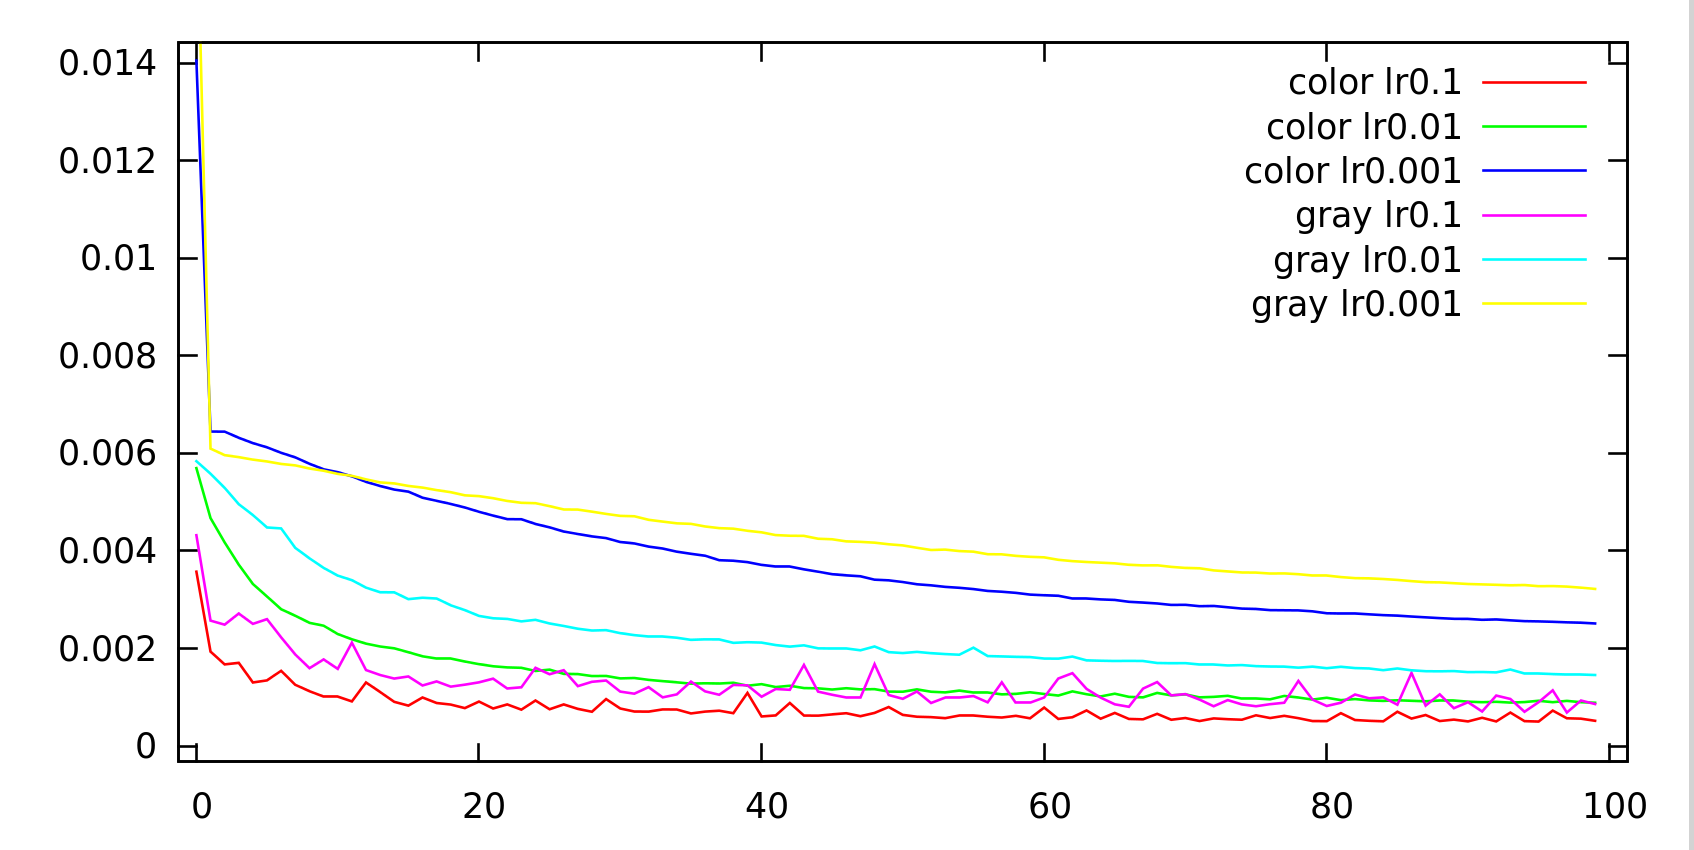
\includegraphics[width=\textwidth]{results/cnn_color_vs_gray.png}
	\caption{Training error for color and gray-value inputs and several learning rates}
	\label{fig:cnn_color_vs_gray}
\end{figure}

Before describing the plot shown in the figure, it shall be substantiated why the error is calculated on the undistorted training images and not on a separate validation set with images showing persons, which are disjoint from those present in the training and test sets. Since the network is never trained on the undistorted training images, also these images can be seen to some extent as kind of validation set even though it contains the same persons, which are presented to the network during the training process. A validation set with images disjoint from the training images and the test images was not used, because it would narrow the number of the latter two kinds of images. Nonetheless calculating the error on the same unseen data every time might give a good estimation of the performance of the network in a more general sense than only for the specific distorted images, which were used in the respective epoch.\\
As indicated by the plot above, the network, which exploits the color information, always performs better than its corresponding counterpart with the same learning rate, which receives only gray-value images as input. This optical impression is confirmed by the mere numbers given in table \ref{tab:cnn_errors_color_vs_gray}, which shows the training error, the training error in pixels, the test error and the test error in pixels up to the 10th decimal place for each of the six tested networks. When speaking about the training error, it is always intended the error on the undistorted training images (although \q{validation set} might be a more appropriate term).

\begin{table}[h!]
\centering
\footnotesize
\begin{tabular}{|l|l|l|l|l|}
	\hline
		\textbf{Setup} & \textbf{Training error} & \textbf{Training error (pixels)} & \textbf{Test error} & \textbf{Test error (pixels)}\\
	\hline
		color lr0.1		& 0.0005185750%4570566914
						& 2.9148470884%15048
						& 0.0009183273%8801671525
						& 3.8789013812%245683
						\\
	\hline
		color lr0.01 	& 0.0008885668%6493293487
						& 3.8155313542%23315
						& 0.0010579627%578808069
						& 4.1633714493%327565
						\\
	\hline
		color lr0.001 	& 0.0025131641%142505522
						& 6.4168279428%29778
						& 0.0023130839%1477012
						& 6.1560999715%39907
						\\
	\hline
		gray lr0.1 		& 0.0008617480%339873435
						& 3.7575097855%95859
						& 0.0012009542%901969344
						& 4.4358127880%4534
						\\
	\hline
		gray lr0.01 	& 0.0014563405%874423343
						& 4.8847399300%94048
						& 0.0015545599%945216019
						& 5.0467723299%393965
						\\
	\hline
		gray lr0.001 	& 0.0032208980%49184056
						& 7.2643784068%44702
						& 0.0029630543%498798487
						& 6.9675449383%862205
						\\
	\hline
	\end{tabular}
	\normalsize
	\caption{Errors for color and gray-value input and several learning rates.}
	\label{tab:cnn_errors_color_vs_gray}
\end{table}

Since each color information using network clearly outperforms its corresponding gray-value image using network, all upcoming networks will take three input maps, one for each color channel, although training a network with three input maps requires more training time than training a network with only 1 input map. Training the color networks took around 45 minutes, whereas the gray-value networks finished the 100th epoch after approximately 30 minutes. The learning rate will be provisionally fixed to 0.1 for the next researched networks, because this learning rate yielded the best results. Before examining the influence of the images' resolution on the networks' performance, table \ref{tab:params_best_color_network} summarizes all parameters of the so far best considered \acp{CNN}.

\begin{table}[h!]
	\footnotesize
	\centering
	\begin{tabular}{ll}
	\hline
		\textbf{Parameter} & \textbf{Value}\\
	\hline
	\hline
		\textbf{Resolution} & $3 \times 96\times128$\\
		\textbf{Learning rate} & 0.1\\
		\textbf{Batch size} & 4\\
		\textbf{Epochs} & 100\\
		\textbf{Trainable parameters} & 6,444,578\\
		\textbf{Execution time} & 2,652s\\
		\textbf{GPU} & GeForce GTX 860m\\
	\hline
	\end{tabular}
	\caption{Parameters for the best color network}
	\label{tab:params_best_color_network}
\end{table}


Figure \ref{fig:structure_of_the_best_color_network} compactly illustrates the structure of the best performing network.

\begin{figure}[h!]
	\scriptsize
	\centering
	\begin{tabular}{|c|}
	\hline
		\textbf{Convolutional Layer}\\
		3 input maps, 32 output maps, filter size $3\times3$, Glorot normal initialization, \ac{ReLU}\\
	\hline
		\textbf{Max Pooling Layer}\\
		pooling size $2\times2$\\
	\hline
		\textbf{Convolutional Layer}\\
		64 output maps, filter size $2\times2$, Glorot normal initialization, \ac{ReLU}\\
	\hline
		\textbf{Max Pooling Layer}\\
		pooling size $2\times2$\\
	\hline
		\textbf{Convolutional Layer}\\
		128 output maps, filter size $2\times2$, Glorot normal initialization, \ac{ReLU}\\
	\hline	
		\textbf{Max Pooling Layer}\\
		pooling size $2\times2$\\
	\hline
		\textbf{Fully Connected Layer}\\
		300 neurons, Glorot normal initialization, sigmoid\\
	\hline
		\textbf{Fully Connected Layer}\\
		200 neurons, Glorot normal initialization, sigmoid\\
	\hline
		\textbf{Output Layer}\\
		30 neurons, Glorot normal initialization\\
	\hline
	\end{tabular}
	\caption{Structure of the best performing color network}
	\label{fig:structure_of_the_best_color_network}
\end{figure}


\subsubsection{Larger Input Image Resolution}

After finding that color information is indeed useful and that the learning rate should be set to a value around $10^{-1}$, it may be a reasonable next step to examine the influence of the images' resolution on the network's performance. Hence, the best performing \ac{CNN} from the previous considerations was compared to an almost identical copy of it. The only difference is that the new network uses larger input images, which now have a resolution of $120\times160$. This means that the total number of free parameters increases from 6,444,578 to 10,322,978. Although the number of parameters for the convolutional layers does not change, there are more connections required to connect the larger output map of the last max pooling layer with all neurons of the first fully connected layer. Figure \ref{fig:cnn_96_vs_120} shows a plot of the training errors for both networks and table \ref{tab:cnn_errors_96_vs_120} lists all error values.

\begin{figure}[h!]
	\centering
	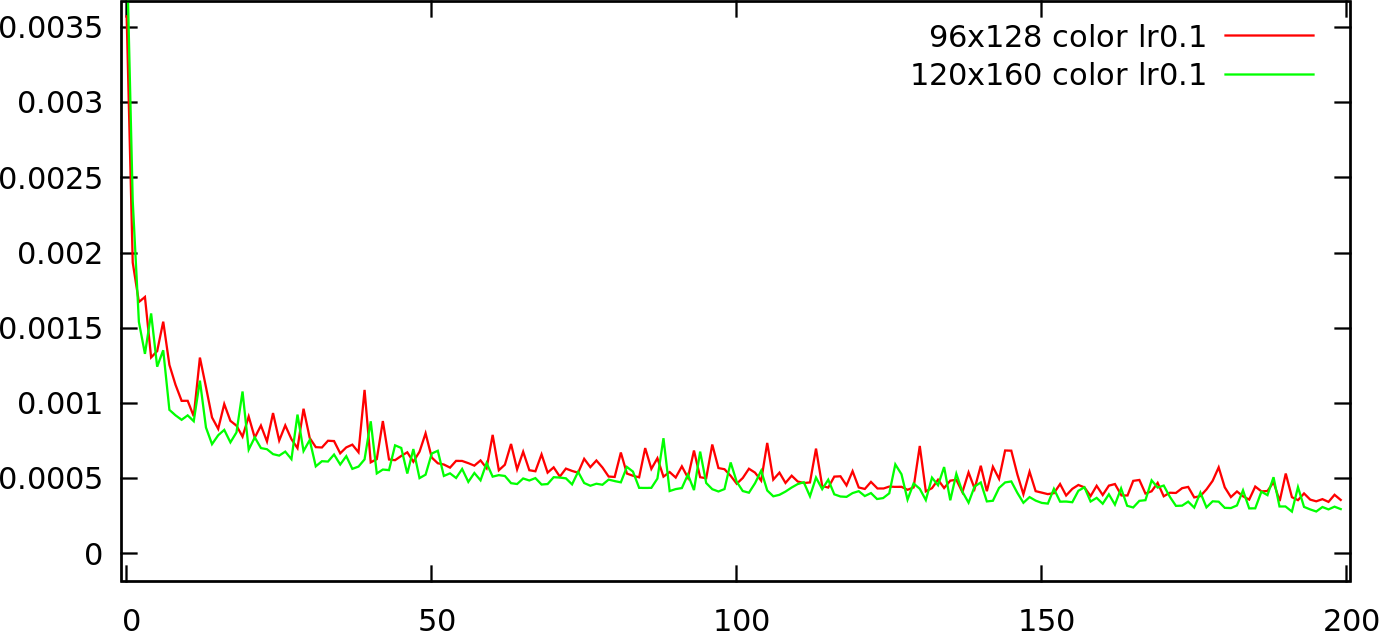
\includegraphics[width=\textwidth]{results/cnn_96vs120.png}
	\caption{Training error for input images of size $96\times128$ and $120\times160$}
	\label{fig:cnn_96_vs_120}
\end{figure}

\begin{table}[h!]
\centering
\footnotesize
\begin{tabular}{|l|l|l|l|l|}
	\hline
		\textbf{Setup} & \textbf{Training error} & \textbf{Training error (pixels)} & \textbf{Test error} & \textbf{Test error (pixels)}\\
	\hline
		$96\times128$	& 0.0003584827%6249689909
						& 2.4235060513%12683
						& 0.0008303526%5135673149
						& 3.6884275565%37974
						\\
	\hline
		$120\times160$ 	& 0.0002973102%3911780993
						& 2.7588298464%051633
						& 0.0007783855%6463537387
						& 4.4639299338%88476
						\\
	\hline
	\end{tabular}
	\normalsize
	\caption{Errors for input images of size $96\times128$ and $120\times160$}
	\label{tab:cnn_errors_96_vs_120}
\end{table}


Both networks were trained for 200 epochs in order to increase the comparability of their long-term behavior. The first 100 epochs of the network with the smaller input maps were adopted from the network presented above. The plot and the error table reveal that the network with input images of size $120\times160$ performs marginally better than the network with input images of size $96\times128$. However, the absolute number of pixels is larger for the network with the larger input images than for the network with the smaller input images, but this is not necessarily a problem, because a deviation of approximately 4.47 pixels in a larger image can be better than a deviation of approximately 3.7 pixels in a smaller image. Even if it is strictly speaking sufficient to look at the normal error values (since both relate to labels in the unit interval), computing the number of pixels, which corresponds to the distance between the true label and the prediction in the original image with a resolution of $480\times640$ pixels, may increase the intuitive understanding and the vividness of the rather abstract error values. As the images with size $96\times128$ are downscaled by a factor of $\frac{1}{5}$ and the images with size $120\times160$ by a factor of $\frac{1}{4}$, the error value belonging to the former images has to be multiplied with 5 and the error value of the latter images with a factor of 4. Table \ref{tab:cnn_errors_400_96_vs_120} shows the resulting values, which again reveal that the \ac{CNN} with the larger input images performs better than the network with the smaller input maps.

\begin{table}[h!]
\centering
\footnotesize
\begin{tabular}{|l|l|l|}
	\hline
		\textbf{Setup} & \textbf{Upscaled Training Error} & \textbf{Upscaled Test Error}\\
	\hline
		$96\times128$	& 12.11753026
						& 18.44213778
						\\
	\hline
		$120\times160$ 	& 11.03531939
						& 17.85571974
						\\
	\hline
	\end{tabular}
	\normalsize
	\caption{Upscaled errors for input images of size $96\times128$ and $120\times160$}
	\label{tab:cnn_errors_400_96_vs_120}
\end{table}


Because of the better performance of the network with the larger input maps, from now on all networks will use the larger resolution despite the expanded computation time. Even larger input images were not used due to computation time and memory space restrictions. Table \ref{tab:params_120_network} shows the updated parameters for the here considered network with the larger input images. An overview about the network structure like in figure \ref{fig:structure_of_the_best_color_network} is not given, because it looks exactly like the one given in the referenced figure.

\begin{table}[h!]
	\footnotesize
	\centering
	\begin{tabular}{ll}
	\hline
		\textbf{Parameter} & \textbf{Value}\\
	\hline
	\hline
		\textbf{Resolution} & $120\times160$\\
		\textbf{Learning rate} & 0.1\\
		\textbf{Batch size} & 4\\
		\textbf{Color} & Yes\\
		\textbf{Epochs} & 200\\
		\textbf{Trainable parameters} & 10.322.978\\
		\textbf{Execution time} & 7563s\\
	\hline
	\end{tabular}
	\caption{Parameters for the network with larger input images ($120\times160$)}
	\label{tab:params_120_network}
\end{table}


\subsubsection{Glorot Uniform Initialization vs. Glorot Normal Initialization}

After making the decisions about the color information, the preliminary learning rate and the resolution of the input images the Glorot normal initialization was opposed to the Glorot uniform initialization. Therefore all layers in the \ac{CNN} used the Glorot uniform initialization introduced in equation \eqref{eq:glorotinitialization} instead of the Glorot normal initialization defined in equation \eqref{eq:glorotinitializationnormal}. Figure \ref{fig:cnn_normal_vs_uniform} shows the training error plots for the best network so far and the network with the uniform initialization. Table \ref{tab:cnn_errors_uniform} presents the corresponding error values after the 200th epoch.

\begin{figure}[h!]
	\centering
	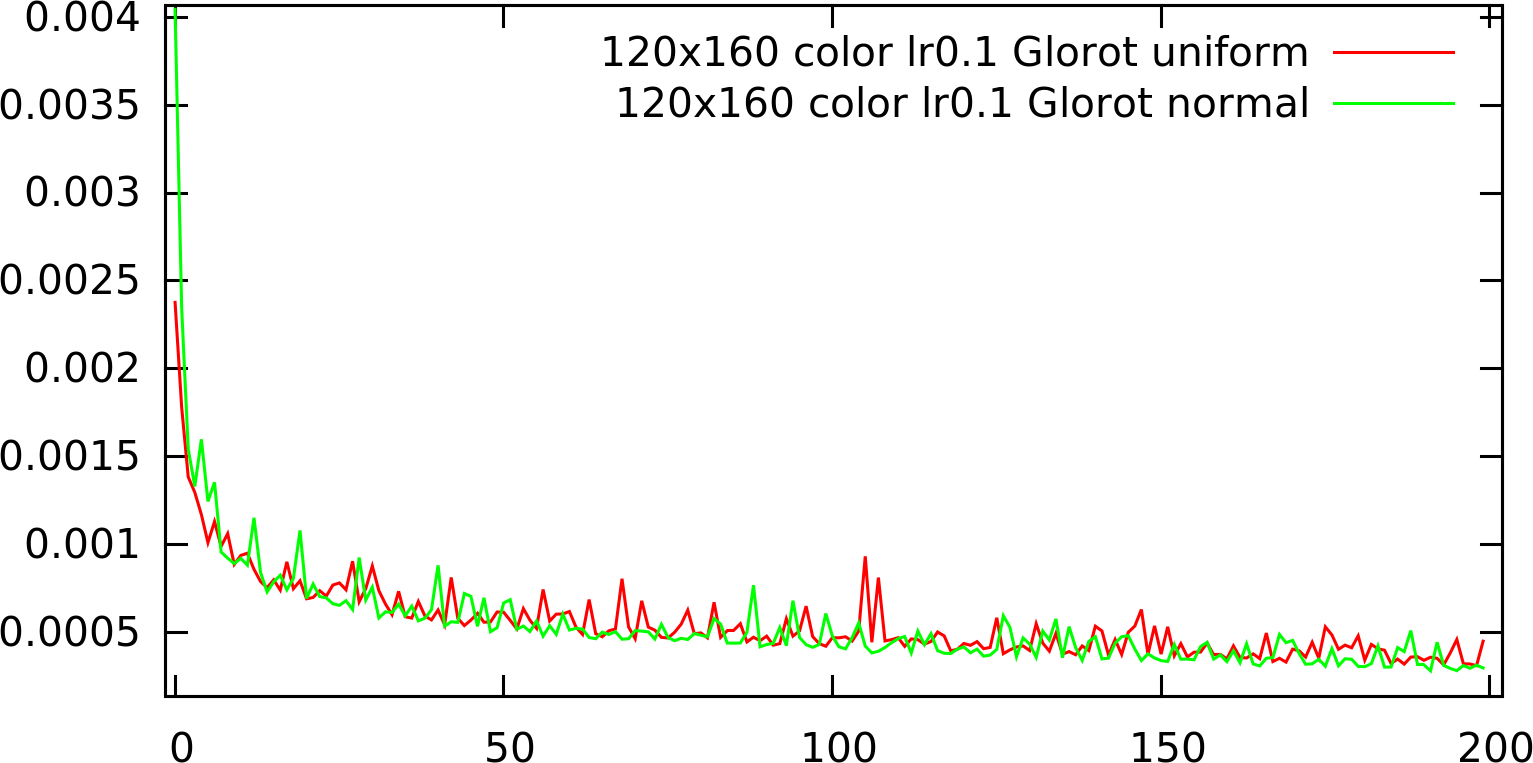
\includegraphics[width=\textwidth]{results/cnn_normal_vs_uniform.png}
	\caption{Glorot uniform initialization vs Glorot normal initialization}
	\label{fig:cnn_normal_vs_uniform}
\end{figure}

\begin{table}[h!]
\centering
\footnotesize
\begin{tabular}{|l|l|l|l|l|}
	\hline
		\textbf{Setup} & \textbf{Training error} & \textbf{Training error (pixels)} & \textbf{Test error} & \textbf{Test error (pixels)}\\
	\hline
		uniform	& 0.0004494951%2272322444
				& 3.3922080038%987215
				& 0.0010167811%809599348
				& 5.1019210335%49454
				\\
	\hline
		normal 	& 0.0002973102%3911780993
				& 2.7588298464%051633
				& 0.0007783855%6463537387
				& 4.4639299338%88476
				\\
	\hline
	\end{tabular}
	\normalsize
	\caption{Errors for the uniform initialization and the normal initialization}
	\label{tab:cnn_errors_uniform}
\end{table}


The values in the table suggest that the network with the Glorot normal initialization performs significantly better than the network with the Glorot uniform distribution. This is not necessarily true, because both shown error curves exhibit strong fluctuations, which render it nearly impossible to claim which one of them is better. However, a decision must be made and since there is no clear winner and since the execution time for both networks is virtually identical (7,563s for the Glorot normal initialization and 7,573s for the Glorot uniform initialization), it was taken the decision to use the Gabor normal initialization in the further considerations.

\subsubsection{Refinement of the Learning Rate}

There were tested only three learning rates in chapter \ref{subsubsec:color_gray_learningrate} in order to find a passably good one for the first examined networks. This chapter, in contrast, is supposed to refine the choice for the learning rate by testing a few more values. Since 0.1 is the best value so far, the tested learning rates are chosen to be close to this value. The training errors over 200 epochs for four networks with the learning rates 0.05, 0.1, 0.15 and 0.2 are depicted in figure \ref{fig:cnn_learningrates}. The corresponding error values for the 200th epoch can be found in table \ref{tab:cnn_errors_learningrates}.\\

\vspace{-0.4cm}
\begin{figure}[h!]
	\centering
	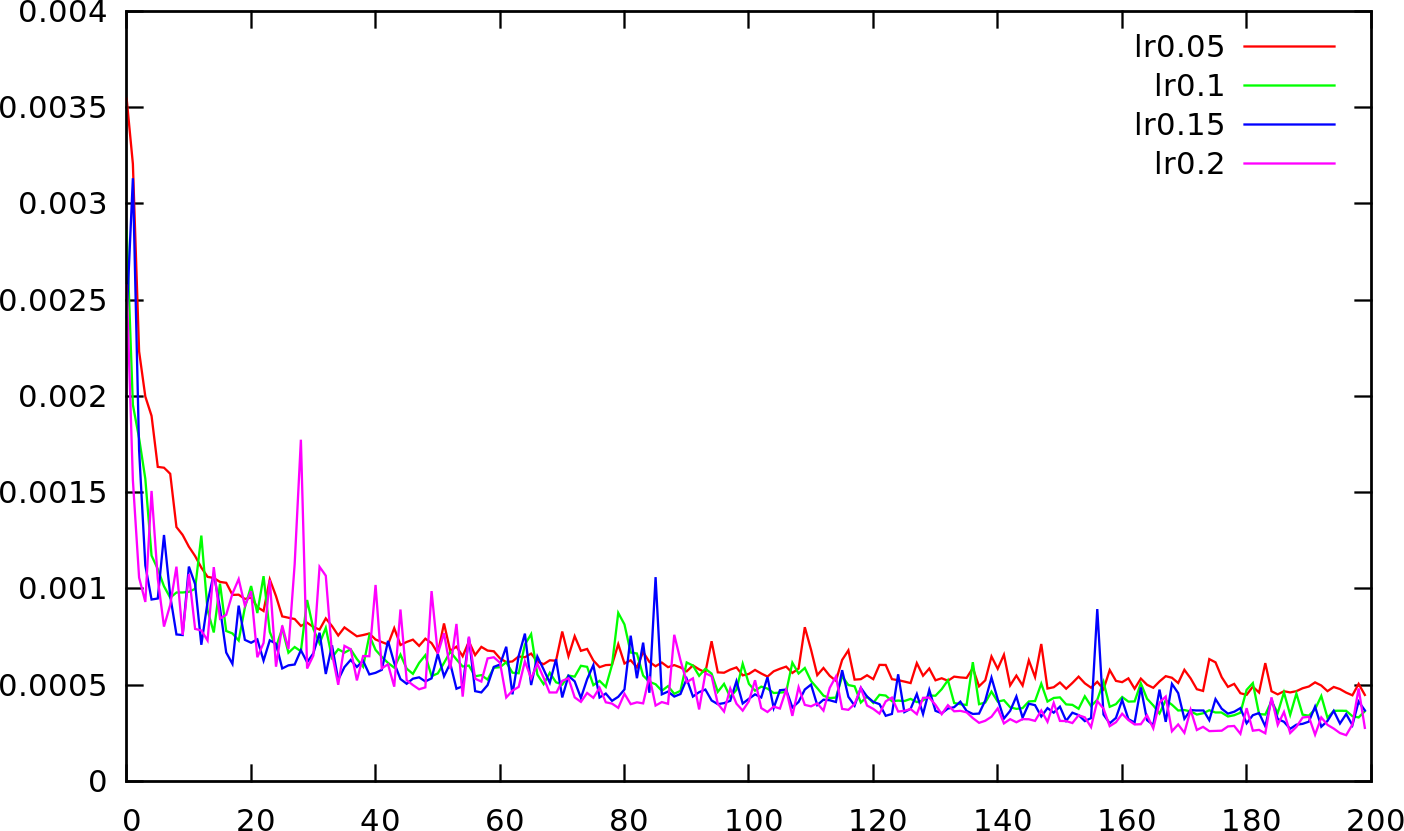
\includegraphics[width=\textwidth]{results/cnn_learningrates.png}
	\caption{4 different learning rates}
	\label{fig:cnn_learningrates}
\end{figure}

\begin{table}[h!]
\centering
\footnotesize
\begin{tabular}{|l|l|l|l|l|}
	\hline
		\textbf{Setup} & \textbf{Training error} & \textbf{Training error (pixels)} & \textbf{Test error} & \textbf{Test error (pixels)}\\
	\hline
		lr 0.05	& 0.0004490067%9969867095
				& 3.3903648877%791865
				& 0.0009108307%2803955448
				& 4.8287955680%28594
				\\
	\hline
		lr 0.1 	& 0.0003645698%9029775866
				& 3.0549941393%7615
				& 0.0008981644%4990660352
				& 4.7951027014%66263
				\\
	\hline
		lr 0.15	& 0.0003688541%2622802283
				& 3.0728920630%95836
				& 0.0009537259%6109530403
				& 4.9411926297%24101
				\\
	\hline
		lr 0.2 	& 0.0002776546%7441035792
				& 2.6660757050%21364
				& 0.0008671437%285547672
				& 4.7115686826%15381
				\\
	\hline
	\end{tabular}
	\normalsize
	\caption{Errors for 4 different learning rates}
	\label{tab:cnn_errors_learningrates}
\end{table}


As indicated by the plot and the error values in the table, larger learning rates produce better results. The red curve, which illustrates the training errors for the network with learning rate 0.05, is clearly worse than all three other curves apart from the violet curve during the first 60 epochs. The violet curve depicts the training errors for the network with the highest learning rate, which is prone to larger fluctuations, because it adapts the weights more strongly to the currently considered training images. After the first 60 epochs the violet curve clearly dominates the red curve disregarding very few exceptions. The other two curves are located somewhere in between the curve of the smallest and the curve of the largest learning rate. However, the blue line (learning rate 0.15) tends to outstrip the green line (learning rate 0.1) even if the results after exactly 200 epochs are slightly better for learning rate 0.1 (green curve). Since it is hard to tell which learning rate is the best choice the networks with learning rate 0.15 and 0.2 were trained for another 200 epochs in order to find a hopefully clear favorite. The plots for both networks for all 400 epochs are shown in figure \ref{fig:cnn_learningrates_400}.

\begin{figure}[h!]
	\centering
	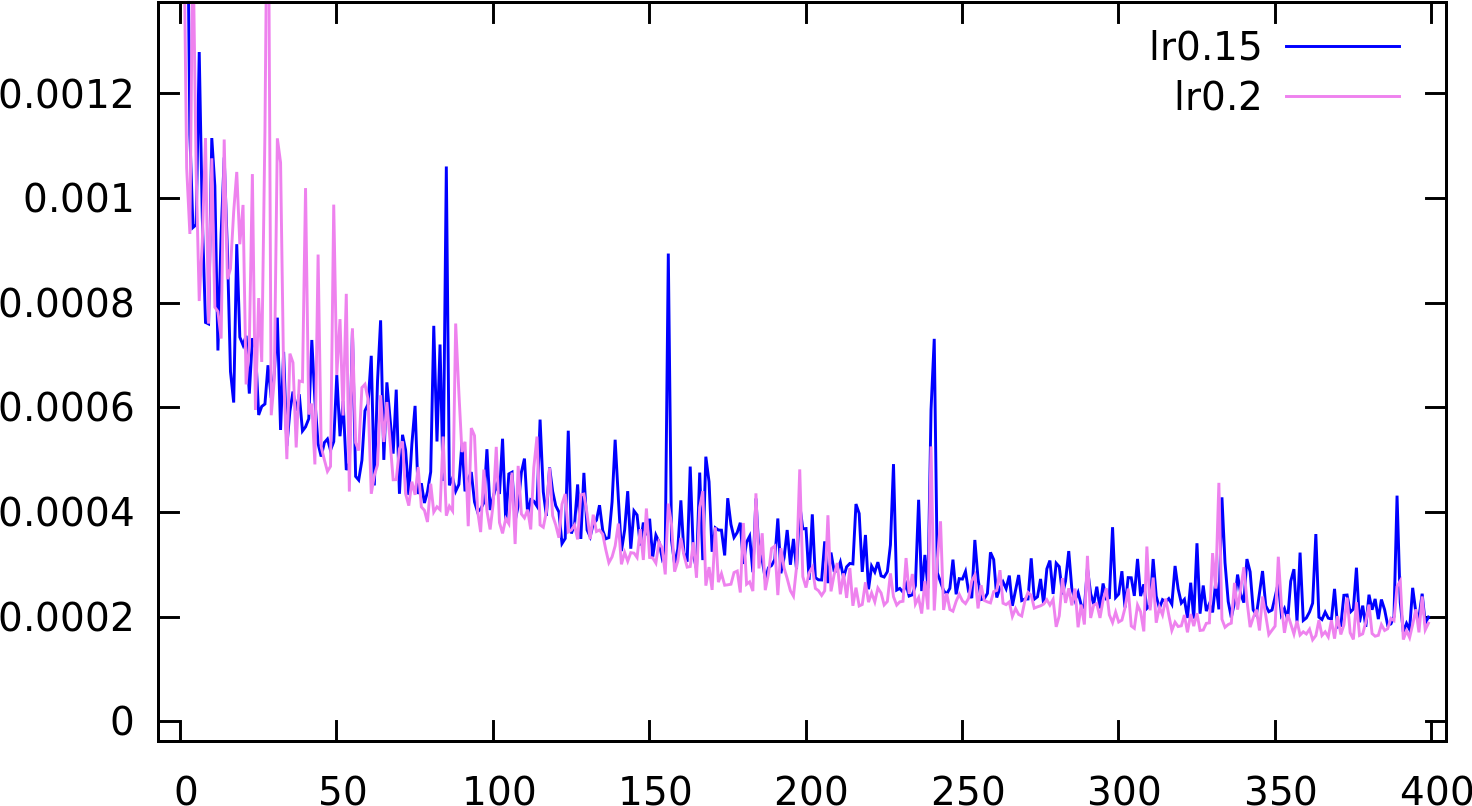
\includegraphics[width=\textwidth]{results/cnn_learningrates_400.png}
	\caption{Learning rates 0.15 and 0.2 for 400 epochs}
	\label{fig:cnn_learningrates_400}
\end{figure}

While the violet curve (learning rate 0.2) has rather a large variance during the first 100 epochs, the blue curve (learning rate 0.15) has a larger variance after the first 100 epochs, whereas the violet curve seems to become more and more smooth. 
\begin{table}[h!]
\centering
\footnotesize
\begin{tabular}{|l|l|l|l|l|}
	\hline
		\textbf{Setup} & \textbf{Training error} & \textbf{Training error (pixels)} & \textbf{Test error} & \textbf{Test error (pixels)}\\
	\hline
		lr 0.15	& 0.0002003702%003399318
				& 2.2648349009%81141
				& 0.0008056193%4514562577
				& 4.5413494949%990385
				\\
	\hline
		lr 0.2 	& 0.0001885331%0514913737
				& 2.1969177253%18342
				& 0.0007700964%0610954016
				& 4.4400977462%6688
				\\
	\hline
	\end{tabular}
	\normalsize
	\caption{200 additional epochs for learning rate 0.15 and 0.2}
	\label{tab:cnn_errors_learningrates_more_epochs}
\end{table}

The error values found in table \ref{tab:cnn_errors_learningrates_more_epochs} show that the network with learning 0.2 is a little bit better than the network with learning rate 0.15. Thus, the learning rate is set to 0.2 for all regarded \acp{CNN} below. Training the network with learning rate 0.2 took 7485s for the first 200 epochs and 7372s for the second 200 epochs and thus 14857s in total.

\subsubsection{Examining Various Activation Functions}

After finding an appropriate learning rate, several different activation function were tried for the two fully connected layers. Next to the sigmoidal activation function, which was used for every network up to now, the tanh activation function and the \ac{ReLU} activation function were tested. Table \ref{tab:cnn_errors_activation_functions} shows the error values after 400 epochs.
\begin{table}[h!]
\centering
\footnotesize
\begin{tabular}{|l|l|l|l|l|}
	\hline
		\textbf{Setup} & \textbf{Training error} & \textbf{Training error (pixels)} & \textbf{Test error} & \textbf{Test error (pixels)}\\
	\hline
		sigmoid	& 0.0001885331%0514913737
				& 2.1969177253%18342
				& 0.0007700964%0610954016
				& 4.4400977462%6688
				\\
	\hline
		tanh 	& 0.0004379020%5824099183
				& 3.3481775178%400253
				& 0.0015209428%3
				& 5.4308023032%455734
				\\
	\hline
		ReLU	& 0.0001769591%8756739605
				& 2.1284161251%328038
				& 0.0008150055%0680460376
				& 4.5677282071%28557
				\\
	\hline
	\end{tabular}
	\normalsize
	\caption{Errors for 3 different activation functions}
	\label{tab:cnn_errors_activation_functions}
\end{table}

While the results for the sigmoidal activation function (trained in 14,857s) are very similar to those of the \ac{ReLU} (trained in 15,261s), the tanh activation function (trained in 15,108s) produces much worse results. These finding is clearly confirmed by the plot of the training error depicted in figure \ref{fig:cnn_sigmoid_vs_tanh_vs_relu}. While the curves of the networks with the sigmoidal activation function and the \ac{ReLU} first approach $2\cdot10^{-4}$ and then fall below it, the curve of the tanh network wiggles around at $4\cdot10^{-4}$.

\begin{figure}[h!]
	\centering
	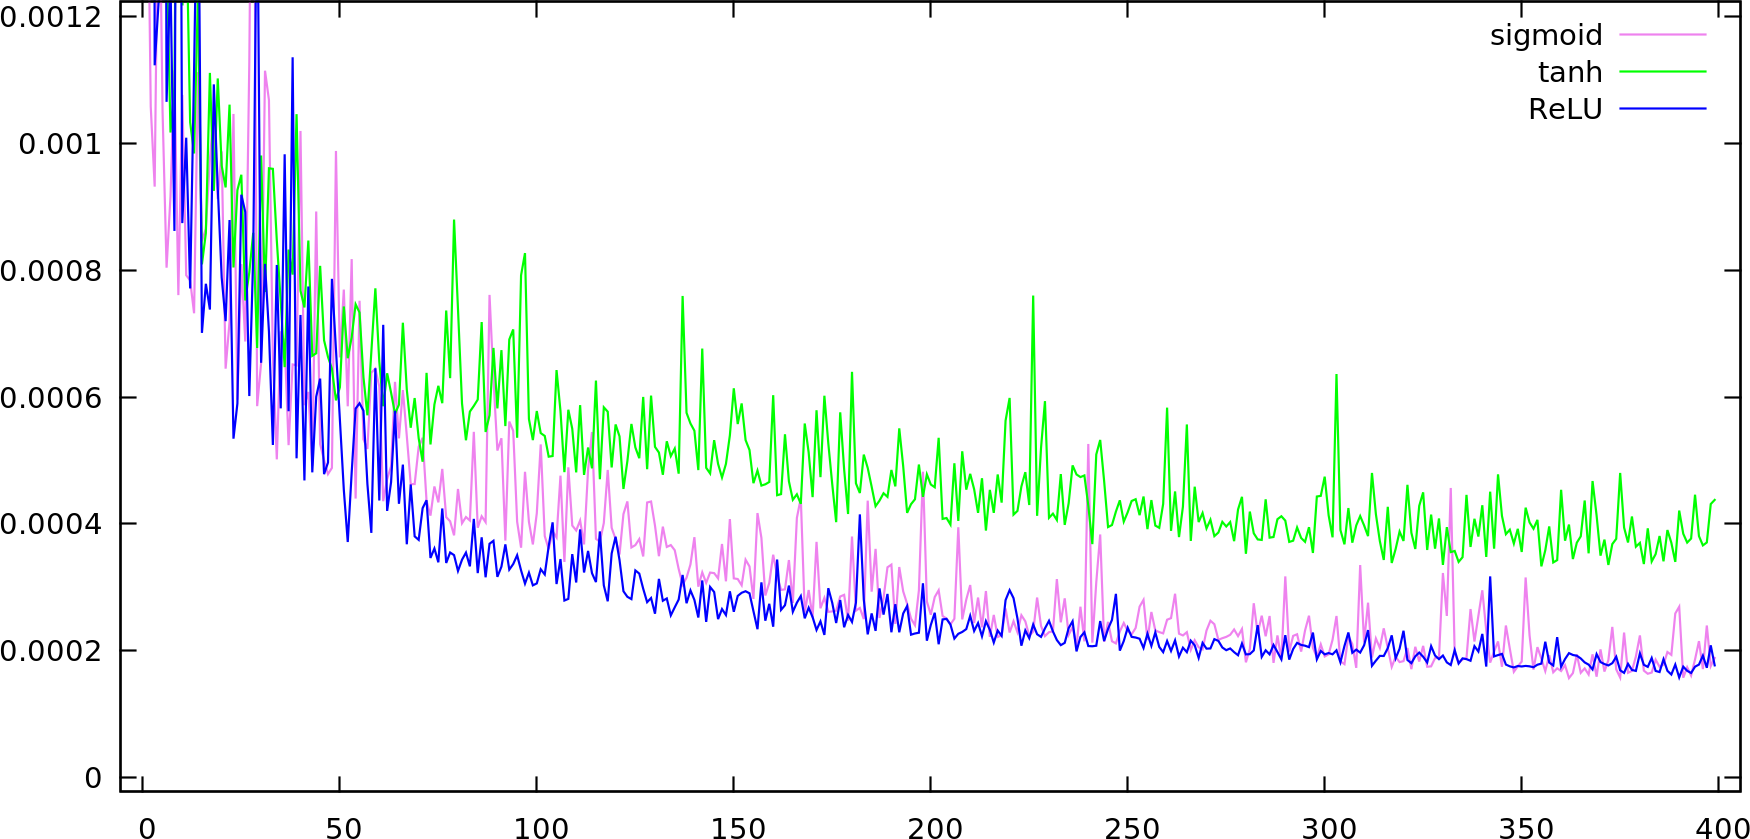
\includegraphics[width=\textwidth]{results/cnn_sigmoid_vs_tanh_vs_relu.png}
	\caption{Sigmoidal, tanh and \ac{ReLU} activation function}
	\label{fig:cnn_sigmoid_vs_tanh_vs_relu}
\end{figure}
\vspace{-0.2cm}
The \ac{ReLU} appears to work a bit better than the sigmoidal activation function, thus the \ac{ReLU} actually should be used from now on. As it happens that some mistakes in the code were not spotted before training the Gabor wavelet based networks, whose results will be presented in chapter \ref{subsec:results_gabornetworks} and which always use the sigmoidal function as activation function for the fully connected layers, the sigmoidal activation function was chosen for all the networks following in this subchapter, which had to be retrained after finishing the training phase of the Gabor networks in order to increase the comparability of both approaches. This should not unduly worsen the performance of the following networks, because the plot shows that the network with the sigmoidal activation function does not perform significantly worse than the \ac{ReLU} network. Thus the network which forms the basis of the networks examined below has the parameter configuration shown in table \ref{tab:params_learningrates_network}.
\vspace{-0.6cm}
\begin{table}[h!]
	\footnotesize
	\centering
	\begin{tabular}{ll}
	\hline
		\textbf{Parameter} & \textbf{Value}\\
	\hline
	\hline
		\textbf{Resolution} & $120\times160$\\
		\textbf{Learning rate} & 0.2\\
		\textbf{Batch size} & 4\\
		\textbf{Color} & Yes\\
		\textbf{Epochs} & 400\\
		\textbf{Trainable parameters} & 10.322.978\\
		\textbf{Execution time} & 14857s\\
	\hline
	\end{tabular}
	\caption{Parameters for the best network, which uses the sigmoidal activation function}
	\label{tab:params_learningrates_network}
\end{table}


\subsubsection{Increasing the Batch Size}

Another training parameter, that can be modified, is the batch size, which defines how many training data points are fed into the network before the weights get updated. Until now the batch size was set to 4, but other choices like 1 or 8 are possible, too. Increasing the batch size leads to fewer computationally intense update steps and thus reduces the time, which is required to train the network for one epoch. Accordingly, decreasing the batch size increases the required computation time due to the larger number of weight updates. Figure \ref{fig:cnn_batchsize} shows, which batch size leads to the lowest training error within 400 epochs.

\begin{figure}[h!]
	\centering
	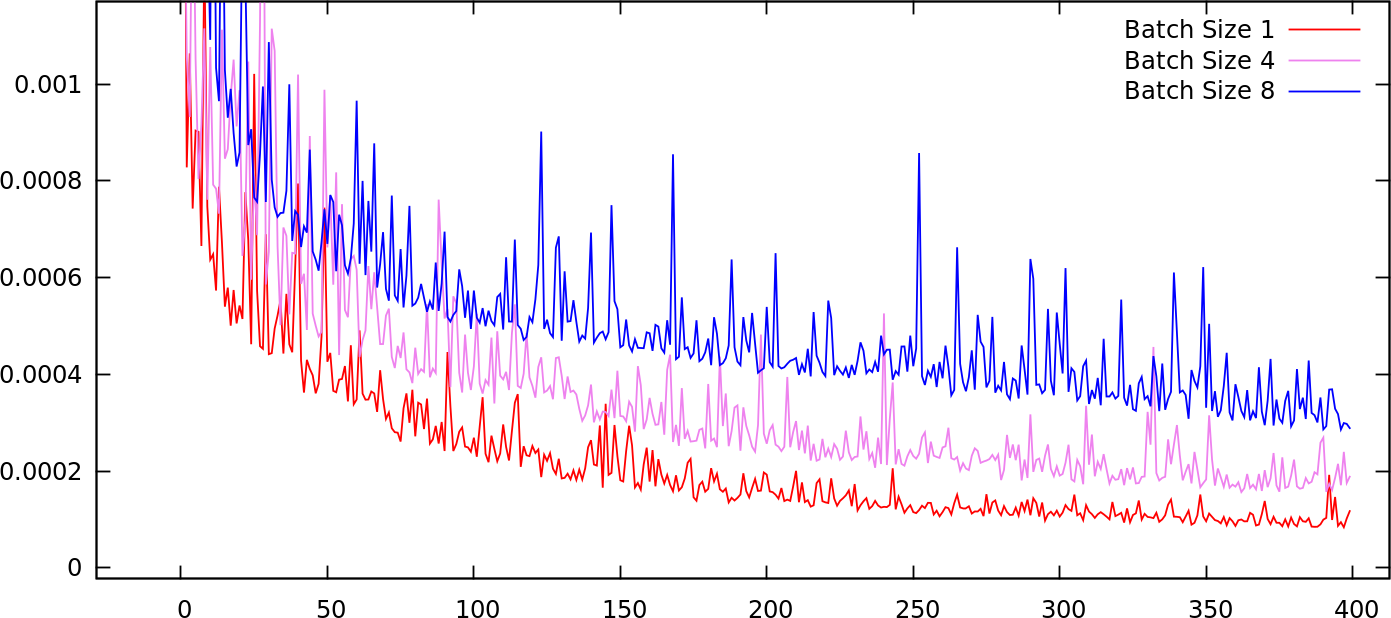
\includegraphics[width=\textwidth]{results/cnn_batchsizes.png}
	\caption{The training error for several different batch sizes}
	\label{fig:cnn_batchsize}
\end{figure}

As can be seen from the plot and the error values in table \ref{tab:cnn_errors_batchsize8}, the network, that was trained with batch size 4, works clearly better than the network with batch size 8. While it took 14,857s to train the network with batch size 4, the network with a twice as large batch size finished its last epoch after 10,182s. If one wants to compare both networks after a certain amount of time, it is reasonable to oppose the training error of the network with batch size 8 after 400 epochs with the training error of the network with batch size 4 after 274 epochs (since $10,182 / 14,857 \approx 0.685$ and $400 \cdot 0.685 = 274$). A look into the plot reveals that the network with batch size 4 after 274 epochs is already better than the other network after 400 epochs. Even larger batch sizes were not tested, because already batch size 8 works worse than batch size 4.\\
Training a network with a batch size smaller than 4 is actually impracticable, because an epoch with weight updates after every single image demands much more computation time than an epoch with weight updates after a larger amount of images. Nevertheless, a single network with batch size 1 was trained in order to find out, whether such a network works even better than the network with batch size 4. This assumption is confirmed by the plot of the training error over all 400 epochs and both the training error and the test error after exactly 400 epochs. The red curve in the plot, which indicates the training error of the network with batch size 1, is not only much less prone to fluctuations than the other two curves but also clearly dominates them in magnitude. Since training the network with batch size 1 requires a lot of computation time, it has been decided to execute it on a more powerful \ac{GPU}. The networks considered so far were trained on a GeForce GTX 860m, whereas the following networks were trained on a more efficient GeForce GTX 780. While the networks with the larger batch sizes could be trained on the weaker GPU in 10,182 and 14,857 seconds, respectively, the batch size 1 network took 14,808 seconds on the more powerful GPU. If the latter network were trained on the weaker GPU, it would take approximately twice as much time as on the GeForce GTX 780. Since many of the following \acp{CNN} require more training time, because they possess much more trainable parameters and because they were trained for more than 400 epochs, all following networks use batch size 4.
\begin{table}[h!]
\centering
\footnotesize
\begin{tabular}{|l|l|l|l|l|}
	\hline
		\textbf{Setup} & \textbf{Training error} & \textbf{Training error (pixels)} & \textbf{Test error} & \textbf{Test error (pixels)}\\
	\hline
		Batch Size 1	& 0.0001174004%3922531784
						& 1.7336237320%041903
						& 0.0007018162%2847345626
						& 4.2386902987%7396
						\\
	\hline
		Batch Size 4 	& 0.0001885331%0514913737
						& 2.1969177253%18342
						& 0.0007700964%0610954016
						& 4.4400977462%6688
						\\
	\hline
		Batch Size 8	& 0.0002890575%2211860557
						& 2.7202706788%546434
						& 0.0008288681%5472372837
						& 4.6064112670%19853
						\\
	\hline
	\end{tabular}
	\normalsize
	\caption{The errors for the networks with batch size 4 and 8, respectively}
	\label{tab:cnn_errors_batchsize8}
\end{table}


\subsubsection{Omitting Max Pooling Layers}
\label{subsubsec:omittingmpl}

As already mentioned in chapter \ref{subsubsec:maxpoolinglayer}, incorporating too many max pooling layers into the \ac{CNN} may be counterproductive, because these layers' purpose is to enable the network to find abstract features anywhere in the image and not at a specific position. Since the output maps of a network without any max pooling layer are so large that there are required more connections between the last convolutional layer and the first fully connected layer than fit into memory, each of the networks tested in this chapter has at least one max pooling layer directly after the first convolutional layer. In fact, exactly two networks, one with one max pooling layer and one with two max pooling layers, have been trained in order to compare them with the best network by now. The max pooling layers of the network, which has two max pooling layers, are positioned behind the first and behind the second convolutional layer.\\
The error plots for all three networks (1, 2 or 3 max pooling layers) are shown in figure \ref{fig:cnn_maxpooling}. It reveals that the network with only one max pooling layer is the best working one with regard to the training error. In this respect the network with two max pooling layers is the second best and thus the network with a max pooling layer behind every convolutional layer the worst.
\begin{table}[h!]
\centering
\footnotesize
\begin{tabular}{|l|l|l|l|l|}
	\hline
		\textbf{Setup} & \textbf{Training error} & \textbf{Training error (pixels)} & \textbf{Test error} & \textbf{Test error (pixels)}\\
	\hline
		3 Layers 	& 0.0001885331%0514913737
					& 2.1969177253%18342
					& 0.0007700964%0610954016
					& 4.4400977462%6688
					\\
	\hline
		2 Layers	& 0.0001630771%2132805066
					& 2.0432264451%103057
					& 0.0006917847%5489765673
					& 4.2082882179%55135
					\\
	\hline
		1 Layer		& 0.0001157520%1004340159
					& 1.7214097295%853419
					& 0.0008192701%2463651886
					& 4.5796632180%42882
					\\
	\hline
	\end{tabular}
	\normalsize
	\caption{The errors for 3, 2 and 1 max pooling layer}
	\label{tab:cnn_errors_maxpooling}
\end{table}

Table \ref{tab:cnn_errors_maxpooling}, however, indicates that the test error is smallest for the network with two max pooling layers, whereas the network with one max pooling layer produces the largest test error. Since the network with two max pooling layers achieved the best test error and since it can be trained in less time than the network with only one max pooling layer (13,210s vs. 24,752s), all following \acp{CNN} will have two max pooling layers, although it did not yield the lowest training error.

\begin{figure}[h!]
	\centering
	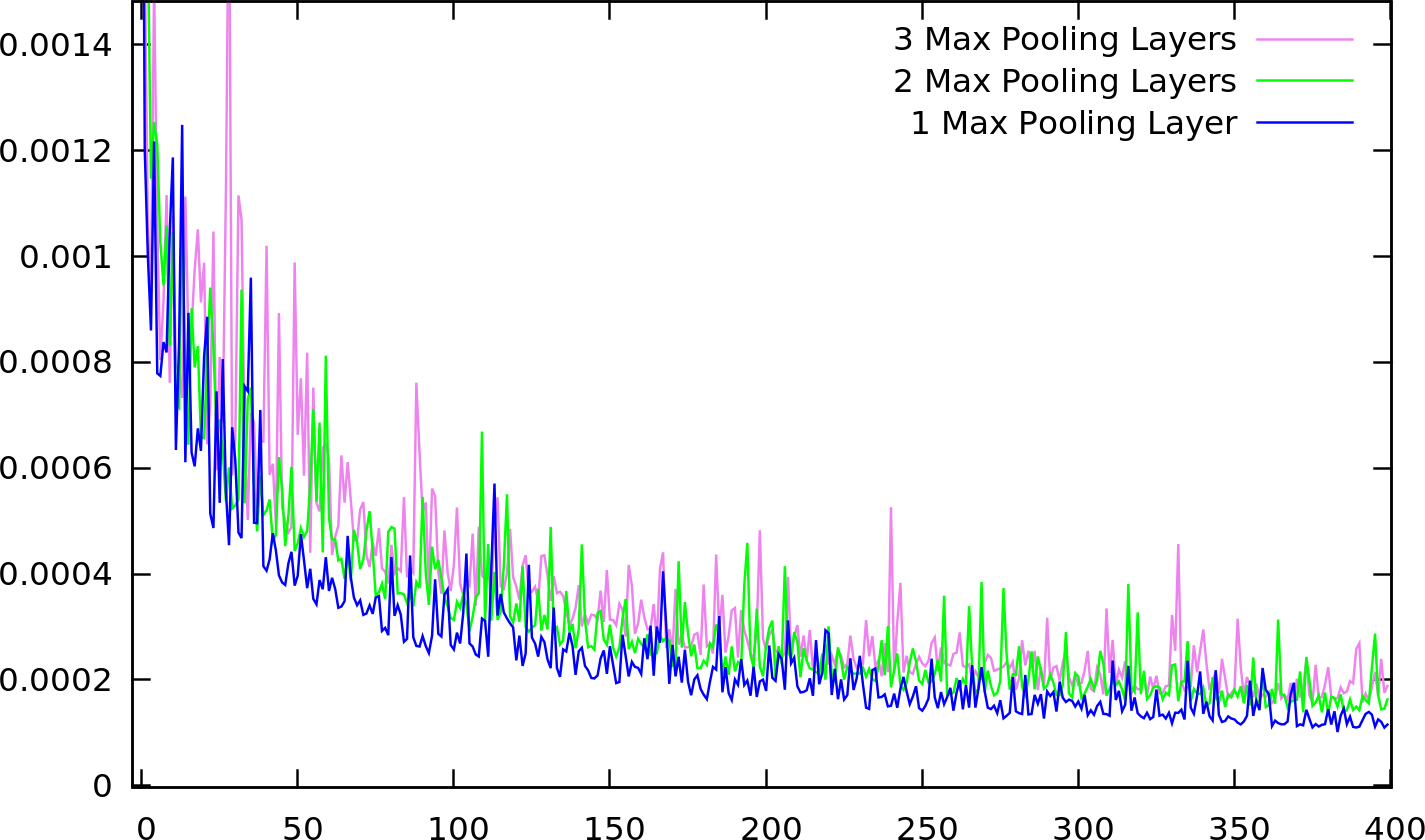
\includegraphics[width=\textwidth]{results/cnn_maxpooling.png}
	\caption{3 max pooling layers, 2 max pooling layers and 1 max pooling layer}
	\label{fig:cnn_maxpooling}
\end{figure}

Table \ref{tab:params_2maxpooling_network} contains the details about the described set-up. The execution time given in the table (13,210s) is smaller than the one in table \myref{tab:params_learningrates_network} (14,857s), because the network belonging to the table above was trained on the GeForce GTX 860m, whereas the here presented network was executed on the more powerful GeForce GTX 780.

\begin{table}[h!]
	\footnotesize
	\centering
	\begin{tabular}{ll}
	\hline
		\textbf{Parameter} & \textbf{Value}\\
	\hline
	\hline
		\textbf{Resolution} & $3 \times 120\times160$\\
		\textbf{Learning rate} & 0.2\\
		\textbf{Batch size} & 4\\
		\textbf{Epochs} & 400\\
		\textbf{Trainable parameters} & 40,966,178\\
		\textbf{Execution time} & 13,210s\\
		\textbf{GPU} & GeForce GTX 780\\
	\hline
	\end{tabular}
	\caption{Parameters for the network with 2 max pooling layers}
	\label{tab:params_2maxpooling_network}
\end{table}


If one used the same hardware for both networks, the training time required for a network with two max pooling layers would be considerably larger than the training time for a network with three max pooling layers, because the former network has over 40 million trainable parameters, whereas the latter network possesses solely approximately a fourth of these parameters. Figure \ref{fig:structure_of_maxpooling_network} illustrates the structure of the network with two max pooling layers.

\begin{figure}[h!]
	\scriptsize
	\centering
	\begin{tabular}{|c|}
	\hline
		\textbf{Convolutional Layer}\\
		3 input maps, 32 output maps, filter size $3\times3$, Glorot normal initialization, \ac{ReLU}\\
	\hline
		\textbf{Max Pooling Layer}\\
		pooling size $2\times2$\\
	\hline
		\textbf{Convolutional Layer}\\
		64 output maps, filter size $2\times2$, Glorot normal initialization, \ac{ReLU}\\
	\hline
		\textbf{Max Pooling Layer}\\
		pooling size $2\times2$\\
	\hline
		\textbf{Convolutional Layer}\\
		128 output maps, filter size $2\times2$, Glorot normal initialization, \ac{ReLU}\\
	\hline
		\textbf{Fully Connected Layer}\\
		300 neurons, Glorot normal initialization, sigmoid\\
	\hline
		\textbf{Fully Connected Layer}\\
		200 neurons, Glorot normal initialization, sigmoid\\
	\hline
		\textbf{Output Layer}\\
		30 neurons, Glorot normal initialization\\
	\hline
	\end{tabular}
	\caption{Structure of the network with 2 max pooling layers}
	\label{fig:structure_of_maxpooling_network}
\end{figure}


\subsubsection{Larger Fully Connected Layers}
\label{subsubsec:largerfc}

The \ac{CNN} presented by Daniel Nouri uses two fully connected layers with 500 neurons each, whereas the respective layers of the networks used in this thesis possess only 300 and 200 neurons in order to reduce the training time and the required memory space. Since more neurons may be necessary to construct an appropriate model, which is capable to solve the problem sufficiently well, the number of neurons in the fully connected layers was increased from 300 to 500 and from 200 to 400, respectively. Figure \ref{fig:cnn_largerfc} shows the error curves of the network with two max pooling layers from the previous chapter with 300 and 200 neurons in the fully connected layers and another network, which is identical to the former one aside from the fact that it has 500 and 400 neurons in the regarded layers.

\begin{figure}[h!]
	\centering
	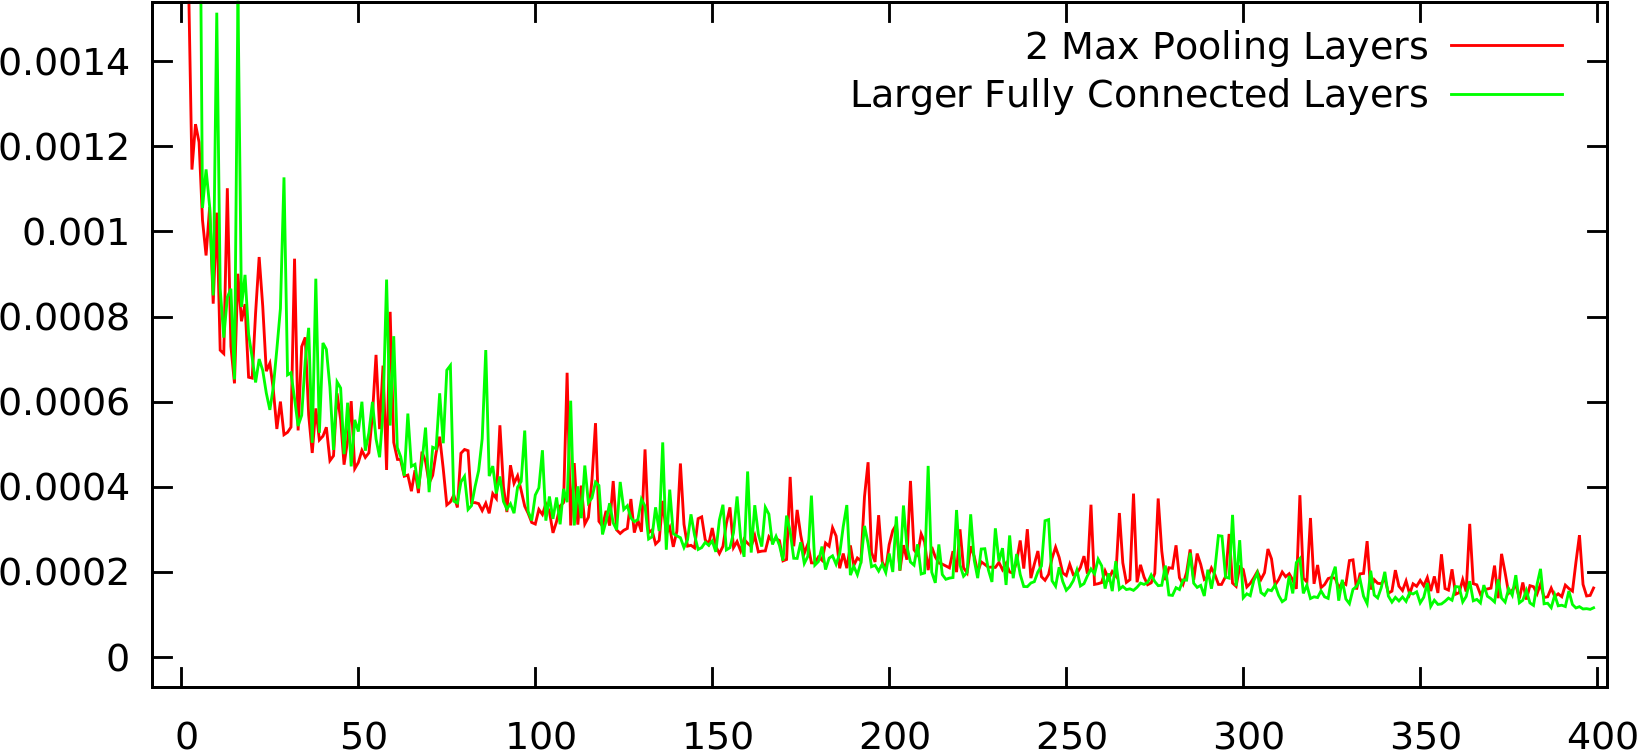
\includegraphics[width=\textwidth]{results/cnn_largerfc.png}
	\caption{300 and 200 neurons vs. 500 and 400 neurons}
	\label{fig:cnn_largerfc}
\end{figure}

The plot and the error values in table \ref{tab:cnn_errors_largerfc} reveal that the performance of both networks is very similar. Since the 68,350,978 trainable parameters of the network with the larger fully connected layers are much more numerous than the 40,966,178 trainable parameters of the network with the fewer neurons in the mentioned layers and since the training time of the smaller network (13,210s) is shorter than the training time of the larger network (15,236s), it has been decided to continue with the smaller network. Another reason which supports this decision is the fact that the test error of the smaller network is better than the the test error of the larger network, albeit the training error of the larger network -- especially towards the end of the training process -- appears to be marginally better.

\begin{table}[h!]
\centering
\footnotesize
\begin{tabular}{|l|l|l|l|l|}
	\hline
		\textbf{Setup} & \textbf{Training error} & \textbf{Training error (pixels)} & \textbf{Test error} & \textbf{Test error (pixels)}\\
	\hline
		500,400	& 0.0001165306%3650443721
				& 1.7271897100%531812
				& 0.0007215457%2749903799
				& 4.2978565150%52053
				\\
	\hline
		300,200	& 0.0001630771%2132805066
				& 2.0432264451%103057
				& 0.0006917847%5489765673
				& 4.2082882179%55135
				\\
	\hline
	\end{tabular}
	\normalsize
	\caption{Errors with and without larger fully connected layers}
	\label{tab:cnn_errors_largerfc}
\end{table}


\subsubsection{Larger Filters}
\label{subsubsec:largerfilters}

The fully connected layers are not the only components of the network, which can be increased in size. The so far used filters of the convolutional layers are rather small, so a network with considerably larger filters was constructed in order to find out, whether small or large filters are more suitable to solve the problem of estimating the position of facial landmarks.
\begin{figure}[h!]
	\centering
	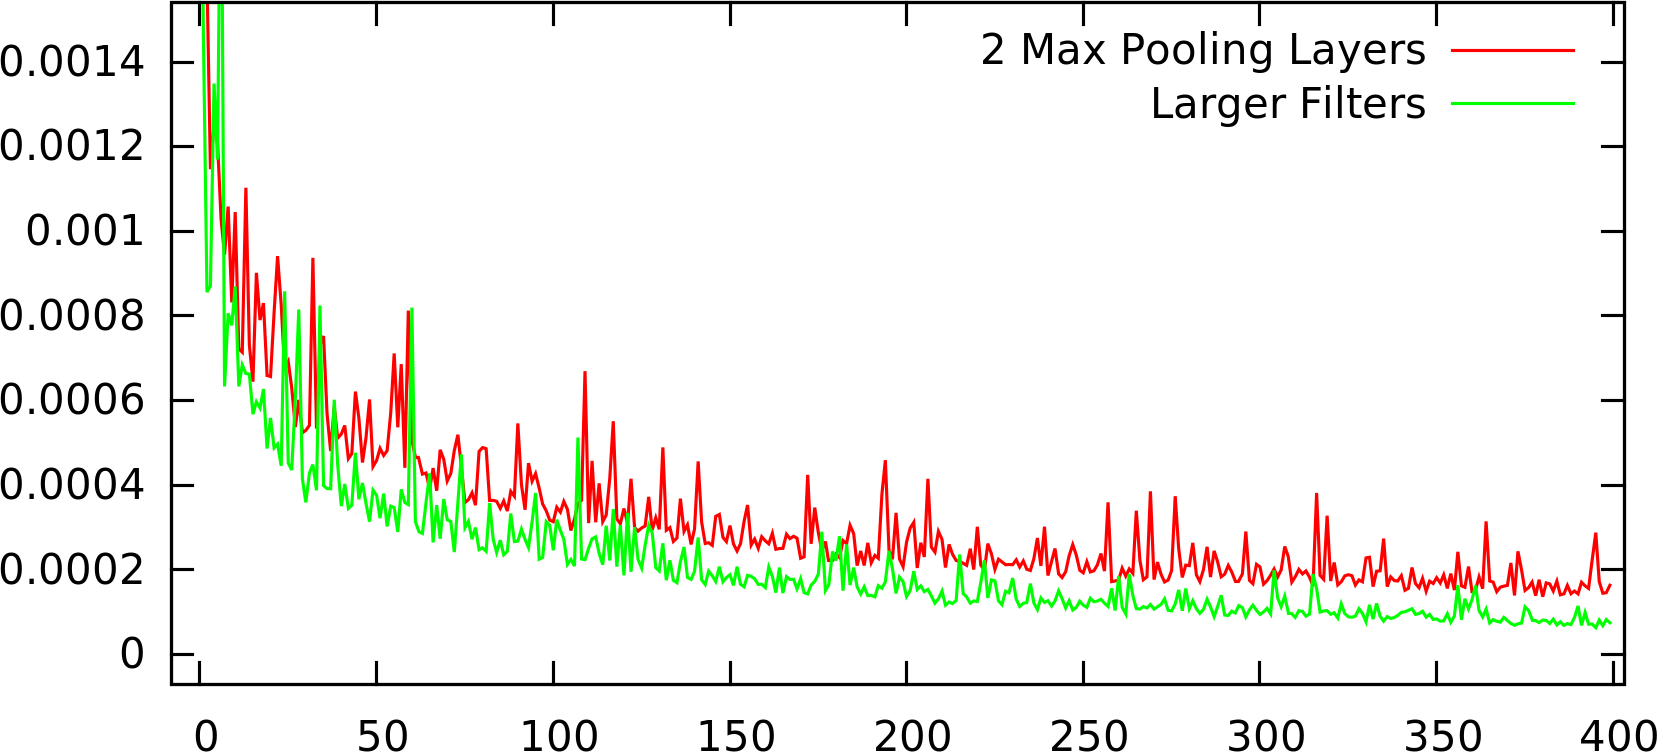
\includegraphics[width=\textwidth]{results/cnn_largerfilters.png}
	\caption{Training error for small and large filters}
	\label{fig:cnn_largerfilters}
\end{figure}
The network, whose error curve is compared to the error curve of the network with two max pooling layers in figure \ref{fig:cnn_largerfilters}, uses filters of size $13\times13$ in the first convolutional layer, filters of size $9\times9$ in the second convolutional layer and filters of size $3\times3$ in the third convolutional layer. Figure \ref{fig:structure_of_the_largerfilters_network} illustrates the tested network with all its layers and filter sizes in a compact form.
\begin{figure}[h!]
	\scriptsize
	\centering
	\begin{tabular}{|c|}
	\hline
		\textbf{Convolutional Layer}\\
		3 input maps, 32 output maps, filter size $13\times13$, Glorot normal initialization, \ac{ReLU}\\
	\hline
		\textbf{Max Pooling Layer}\\
		pooling size $2\times2$\\
	\hline
		\textbf{Convolutional Layer}\\
		64 output maps, filter size $9\times9$, Glorot normal initialization, \ac{ReLU}\\
	\hline
		\textbf{Max Pooling Layer}\\
		pooling size $2\times2$\\
	\hline
		\textbf{Convolutional Layer}\\
		128 output maps, filter size $3\times3$, Glorot normal initialization, \ac{ReLU}\\
	\hline
		\textbf{Fully Connected Layer}\\
		300 neurons, Glorot normal initialization, sigmoid\\
	\hline
		\textbf{Fully Connected Layer}\\
		200 neurons, Glorot normal initialization, sigmoid\\
	\hline
		\textbf{Output Layer}\\
		30 neurons, Glorot normal initialization\\
	\hline
	\end{tabular}
	\caption{Structure of the  network with larger filters}
	\label{fig:structure_of_the_largerfilters_network}
\end{figure}
\\
The plot already indicates that the network with the larger filters performed significantly better than the network with the small filters. The error values found in table \ref{tab:cnn_errors_largerfilters} partly confirm this, because the training error is the smallest training error observed so far. The test error, on the other hand, is a little bit worse than the test error of the network with the smaller filters. 
\begin{table}[h!]
\centering
\footnotesize
\begin{tabular}{|l|l|l|l|l|}
	\hline
		\textbf{Setup} & \textbf{Training error} & \textbf{Training error (pixels)} & \textbf{Test error} & \textbf{Test error (pixels)}\\
	\hline
		small filters	& 0.0001630771%2132805066
						& 2.0432264451%103057
						& 0.0006917847%5489765673
						& 4.2082882179%55135
						\\
	\hline
		large filters	& 0.0000744130%66248028839
						& 1.3802081350%10636
						& 0.0006956846%0248102819
						& 4.2201333893%03509
						\\
	\hline
	\end{tabular}
	\normalsize
	\caption{Errors with and without larger filters}
	\label{tab:cnn_errors_largerfilters}
\end{table}

Even if it is well possible that the network with the larger filters tends to overfit the training data, it was trained for another 600 epochs in order to discover how much room for improvement there is. Before the results of the network after the 1,000th epoch are revealed, all important information about the network, which are not already contained in figure \ref{fig:structure_of_the_largerfilters_network}, are presented in table \ref{tab:cnn_params_largerfilters}.

\begin{table}[h!]
	\footnotesize
	\centering
	\begin{tabular}{ll}
	\hline
		\textbf{Parameter} & \textbf{Value}\\
	\hline
	\hline
		\textbf{Resolution} & $3 \times 120\times160$\\
		\textbf{Learning rate} & 0.2\\
		\textbf{Batch size} & 4\\
		\textbf{Epochs} & 400 + 600\\
		\textbf{Trainable parameters} & 25,320,994\\
		\textbf{Execution time (Epoch 0 - 400)} & 15,801s\\
		\textbf{Execution time (Epoch 400 - 1000)} & 23.612s\\
		\textbf{GPU} & GeForce GTX 780\\
	\hline
	\end{tabular}
	\caption{Parameters for the network with larger filters}
	\label{tab:cnn_params_largerfilters}
\end{table}


Table \ref{tab:cnn_errors_largerfilters_1000} and figure \ref{fig:cnn_largerfilters_1000} reveals that the training error got extremely small after 1,000 epochs. However, the number 0.0000405108 is relatively large, considering that the training error dropped to 0.0000276421 in epoch 999, which corresponds to a deviation of approximately 0.84 pixels. Hence, the network is able to fit the training data very well.
\begin{table}[h!]
\centering
\footnotesize
\begin{tabular}{|l|l|l|l|l|}
	\hline
		\textbf{Setup} & \textbf{Training error} & \textbf{Training error (pixels)} & \textbf{Test error} & \textbf{Test error (pixels)}\\
	\hline
		small filters		& 0.0001630771%2132805066
							& 2.0432264451%103057
							& 0.0006917847%5489765673
							& 4.2082882179%55135
							\\
	\hline
		large filters 400	& 0.0000744130%66248028839
							& 1.3802081350%10636
							& 0.0006956846%0248102819
							& 4.2201333893%03509
							\\
	\hline
		large filters 1000	& 0.0000405108%36752935275
							& 1.0183699823%124908
							& 0.0007615470%541692818
							& 4.4153827225%659175
							\\
	\hline
	\end{tabular}
	\normalsize
	\caption{Errors with larger filters after 1000 epochs}
	\label{tab:cnn_errors_largerfilters_1000}
\end{table}
\\
Unfortunately, there is also a downside. The test error of the network does not decrease at all, in contrast, it is even slightly larger after 1,000 epochs than after 400 epochs for both the network with the larger filters and the network with the small filters. Apparently, the current network configuration leads to overfitting, i.e. the landmarks in the training images can be estimated very precisely whereas the generalization to images with unseen persons does not function well.

\begin{figure}[h!]
	\centering
	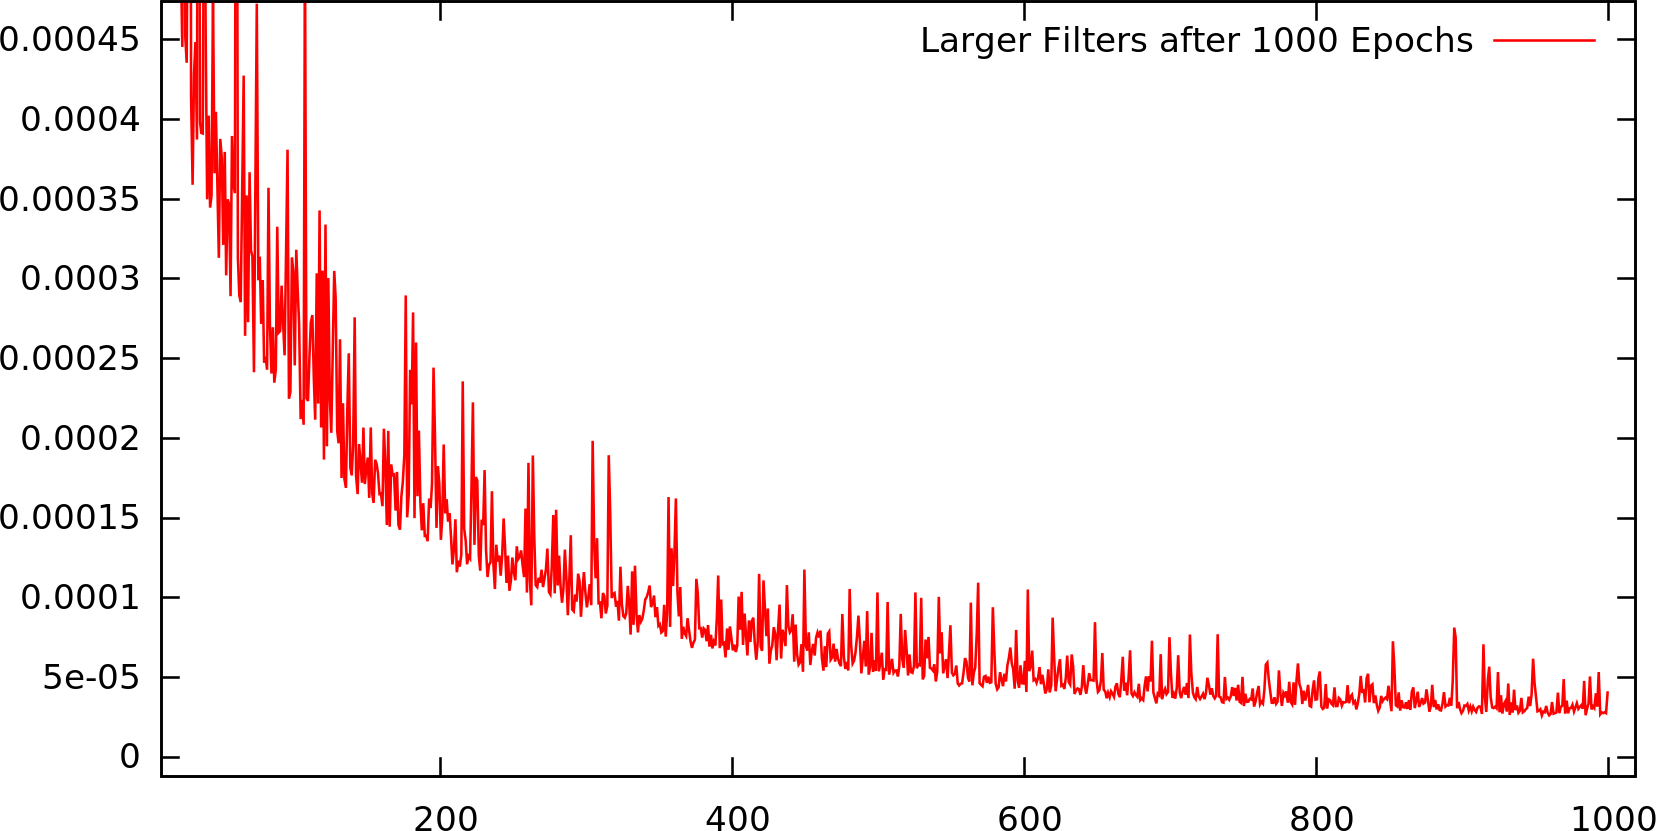
\includegraphics[width=\textwidth]{results/cnn_largerfilters_1000.png}
	\caption{Training error of the network with the larger filters for 1,000 epochs}
	\label{fig:cnn_largerfilters_1000}
\end{figure}

\subsubsection{Larger Filters and Larger Fully Connected Layers}

After finding that the training error is very small and that the test error is still relatively large for both the network with larger fully connected layers and the network with larger filters in the convolutional layers, a combination of both approaches was tried in a last experiment with a conventional \ac{CNN}. Thus, a network with the same number of neurons in the fully connected layers as in chapter \ref{subsubsec:largerfc} and the same filter sizes as in chapter \ref{subsubsec:largerfilters} was trained for 1,000 epochs, yielding the results contained in table \ref{tab:cnn_errors_largenet}.

\begin{table}[h!]
\centering
\footnotesize
\begin{tabular}{|l|l|l|l|l|}
	\hline
		\textbf{Setup} & \textbf{Training error} & \textbf{Training error (pixels)} & \textbf{Test error} & \textbf{Test error (pixels)}\\
	\hline
		large layers	& 0.0001165306%3650443721
						& 1.7271897100%531812
						& 0.0007215457%2749903799
						& 4.2978565150%52053
						\\
	\hline
		large filters	& 0.0000405108%36752935275
						& 1.0183699823%124908
						& 0.0007615470%541692818
						& 4.4153827225%659175
						\\
	\hline
		large network	& 0.0000341614%50477226126
						& 0.9351647620%69759
						& 0.0007047047%9445130206
						& 4.2474042352%89282
						\\
	\hline
	\end{tabular}
	\normalsize
	\caption{Errors with larger filters and larger layers after 1000 epochs}
	\label{tab:cnn_errors_largenet}
\end{table}


The training error of the so called large network, whose curve over all 1,000 epochs is displayed in figure \ref{fig:cnn_largenet_1000}, is remarkably small, but still the test error is approximately as large as for the last two considered network types (either only larger fully connected layers or only larger filters). All three test error values are around $7^{-4}$, which corresponds to approximately 4 pixels. Apparently, the architecture of the here examined \acp{CNN} is not suitable to solve the problem of facial landmark estimation to a satisfactory extent. For this reason, it is reasonable to try to reduce the test error by constructing a model with a different structure.
\begin{figure}[h!]
	\centering
	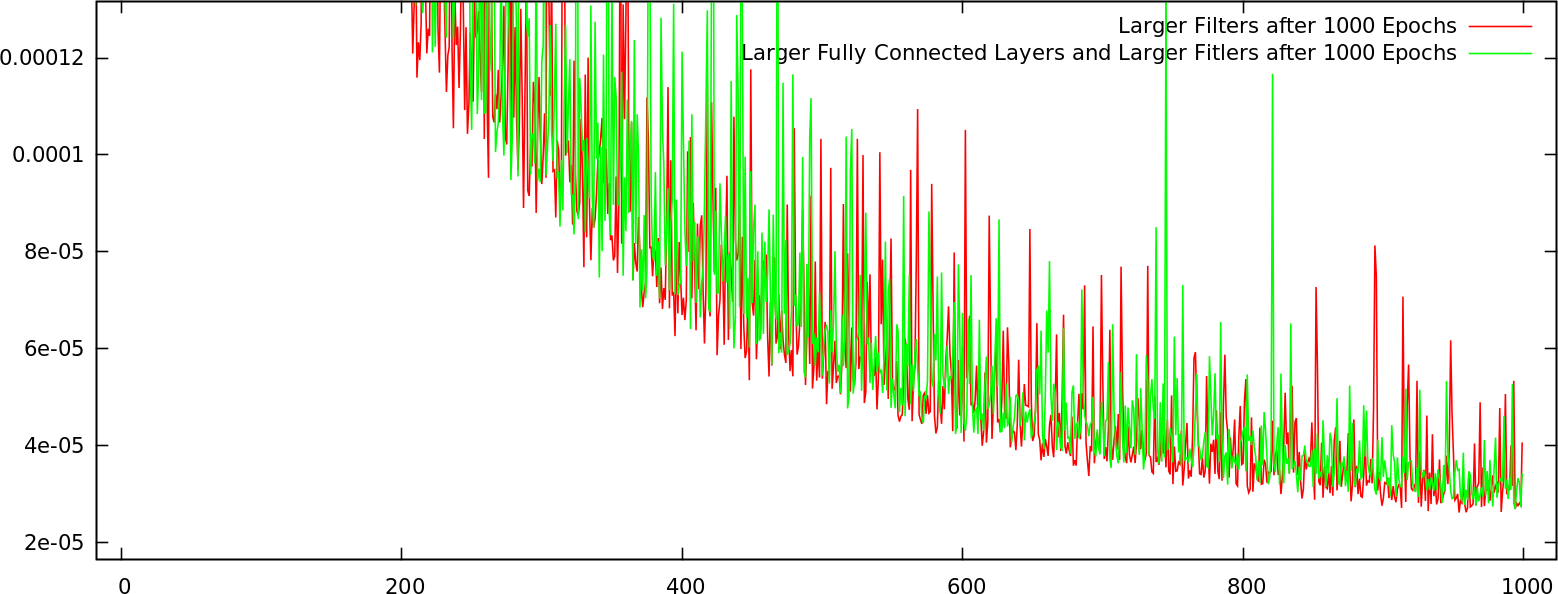
\includegraphics[width=\textwidth]{results/cnn_largenet.png}
	\caption{Training error of the large network for 1,000 epochs}
	\label{fig:cnn_largenet_1000}
\end{figure}

Before continuing the research for a more adequate model, all important information about the large network like the number of trainable parameters and the size of the filters in the convolutional layers is summarized in table \ref{tab:cnn_params_largenet} and figure \ref{fig:cnn_structure_largenet}.

\begin{table}[h!]
	\footnotesize
	\centering
	\begin{tabular}{ll}
	\hline
		\textbf{Parameter} & \textbf{Value}\\
	\hline
	\hline
		\textbf{Resolution} & $3 \times 120\times160$\\
		\textbf{Learning rate} & 0.2\\
		\textbf{Batch size} & 4\\
		\textbf{Epochs} & 1000\\
		\textbf{Trainable parameters} & 42,132,994\\
		\textbf{Execution time} & 42,965s\\
		\textbf{GPU} & GeForce GTX 780\\
	\hline
	\end{tabular}
	\caption{Parameters for the large network}
	\label{tab:cnn_params_largenet}
\end{table}


\begin{figure}[h!]
	\scriptsize
	\centering
	\begin{tabular}{|c|}
	\hline
		\textbf{Convolutional Layer}\\
		3 input maps, 32 output maps, filter size $13\times13$, Glorot normal initialization, \ac{ReLU}\\
	\hline
		\textbf{Max Pooling Layer}\\
		pooling size $2\times2$\\
	\hline
		\textbf{Convolutional Layer}\\
		64 output maps, filter size $9\times9$, Glorot normal initialization, \ac{ReLU}\\
	\hline
		\textbf{Max Pooling Layer}\\
		pooling size $2\times2$\\
	\hline
		\textbf{Convolutional Layer}\\
		128 output maps, filter size $3\times3$, Glorot normal initialization, \ac{ReLU}\\
	\hline
		\textbf{Fully Connected Layer}\\
		500 neurons, Glorot normal initialization, sigmoid\\
	\hline
		\textbf{Fully Connected Layer}\\
		400 neurons, Glorot normal initialization, sigmoid\\
	\hline
		\textbf{Output Layer}\\
		30 neurons, Glorot normal initialization\\
	\hline
	\end{tabular}
	\caption{Structure of the large network}
	\label{fig:cnn_structure_largenet}
\end{figure}


Finally, figure \ref{fig:predictions_largenet} illustrates the performance of the network by showing the network's predictions for two training images in subfigure \ref{fig:predictions_largenet_training} and its predictions for two unseen test images in subfigure \ref{fig:predictions_largenet_test}. The black crosses represent the true labels, whereas the white crosses, which are connected with the black crosses by a gray line, represent the predictions of the network. The images were cropped to a resolution of $240\times320$ in order to focus on the important area of the images, which contains the faces.

\begin{figure}[h!]
	\centering
	
	% training images
	\begin{subfigure}[t]{0.5\textwidth}
		\centering
		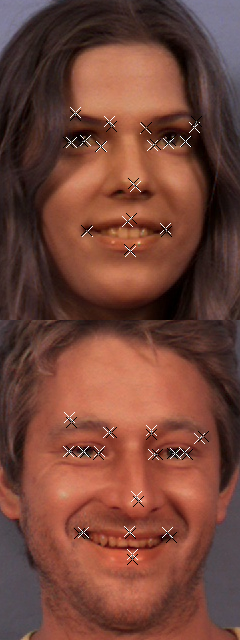
\includegraphics[width=0.78\textwidth]{predictions/predictions_largenet_train.png}
		\caption{Training Predictions}
		\label{fig:predictions_largenet_training}
	\end{subfigure}
	% test images
	\begin{subfigure}[t]{0.49\textwidth}
		\centering
		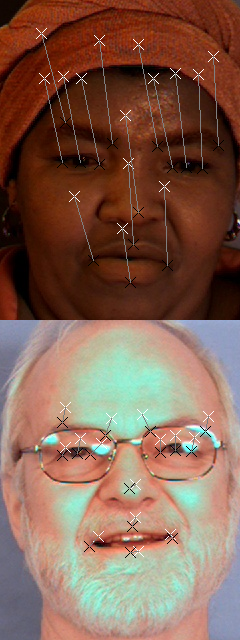
\includegraphics[width=0.78\textwidth]{predictions/predictions_largenet_test.png}
		\caption{Test Predictions}
		\label{fig:predictions_largenet_test}
	\end{subfigure}
	
	\caption{Predictions of the large network}
	\label{fig:predictions_largenet}
\end{figure}


%Largenet Gray:
% Training: 2.9640416365046682e-05 0.8710882038836222
% Test: 0.00071063025293524021 4.265223848186886
% Plot: images/results/largenet_color_vs_gray.png
% Training Time: 30697s on cuda01
% nb of parameters: TBD
% Not sure, whether this should be added here or at the end of the Gabor chapter for a comparison
\newpage
\subsection{Gabor Networks}
\label{subsec:results_gabornetworks}

The conventionally trained \acp{CNN} examined so far were able to produce very good predictions on the training images, but they did not generalize well. For this reason, a different kind of network based on Gabor wavelets was constructed in order to figure out, whether the test error can be decreased more strongly than the up to now regarded \acp{CNN} are capable of. A description of the general structure of the Gabor wavelet based networks can be found in chapter \myref{subsec:gaborcnns}, whereas details about the implementation of the Gabor networks in Keras are illuminated in the appendix \myref{app:implementationremarks}. This chapter presents the precise configurations and the results for a series of Gabor wavelet based networks.

\subsubsection{Initial Gabor Network}

Initially, only Gabor networks with a single merging operation (absolute value or phase) were examined. However, while doing so, several mistakes in the code were spotted and corrected one after the other. As it happens, the first correctly working network turned out to use both merging operations. Hence, the initial Gabor network, which is modified step by step in order to improve its performance steadily, also relies on both merging operations, but later on also networks with only one merging operation are tested and compared to the network with both operations. Furthermore, the initial network does not use any max pooling layers and takes advantage of the color information. Its three input maps have a size of $96\times128$.\\
The 80 output maps of the Gabor layer are as well the input maps of a convolutional layer, which produces 32 output maps by filtering the 80 input maps with $32\cdot80 = 2560$ $3\times3$-filters in total. These 32 output maps are not max pooled, but immediately forwarded to a fully connected layers with 300 neurons, which on its part is connected to another fully connected layer with 200 neurons. The final output layer contains 30 neurons, each of which is connected to all 200 neurons of the preceding fully connected layer. Figure \ref{fig:gabor_structure_initial_network} illustrates the network architecture graphically.

\begin{figure}[h!]
	\scriptsize
	\centering
	\begin{tabular}{|c|}
	\hline
		\textbf{Gabor Layer}\\
		3 input maps, 80 output maps, absolute value and phase, ReLU\\
		filter sizes: $27 \times 27$, $31 \times 31$, $39 \times 39$, $47 \times 47$ and $55 \times 55$\\
	\hline
		\textbf{Convolutional Layer}\\
		80 input maps, 32 output maps, filter size $3\times3$, Glorot normal initialization, \ac{ReLU}\\
	\hline
		\textbf{Fully Connected Layer}\\
		300 neurons, Glorot normal initialization, sigmoid\\
	\hline
		\textbf{Fully Connected Layer}\\
		200 neurons, Glorot normal initialization, sigmoid\\
	\hline
		\textbf{Output Layer}\\
		30 neurons, Glorot normal initialization\\
	\hline
	\end{tabular}
	\caption{Structure of the initial Gabor network}
	\label{fig:gabor_structure_initial_network}
\end{figure}


The network was trained for 1,000 epochs, which required 96,055s of computation time on the faster \ac{GPU} as indicated by table \ref{tab:params_initial_gabor_network}. 
\begin{table}[h!]
	\footnotesize
	\centering
	\begin{tabular}{ll}
	\hline
		\textbf{Parameter} & \textbf{Value}\\
	\hline
	\hline
		\textbf{Resolution} & $3 \times 96\times128$\\
		\textbf{Learning rate} & 0.1\\
		\textbf{Batch size} & 4\\
		\textbf{Epochs} & 1000\\
		\textbf{Trainable parameters} & 65,369,602\\
		\textbf{Execution time} & 96,055s\\
		%\textbf{Execution time (Epoch 1000 - 1500)} & 47345s\\
		\textbf{GPU} & GeForce GTX 780\\
	\hline
	\end{tabular}
	\caption{Parameters for the initial Gabor network}
	\label{tab:params_initial_gabor_network}
\end{table}

The reasons for this comparatively large amount of time are the huge number of parameters (65,369,602) due to the missing dimensionality reduction because of the absent max pooling layers and the costly convolutions with very large filters. The convolutional layer after the Gabor layer consists of 32 output maps with a size of $92 \times 132$ neurons, all of which have to be connected with each of the 300 neurons in the first fully connected layer. This alone necessitates over 99\% of the connections (65,280,300 of 65,369,602) and a large part of the computation time.
Figure \ref{fig:gabor_initial_network} shows the plot of the network's training error. The training error and the test after the 1,000th epoch can be found in table \ref{tab:gabor_errors_initial_network}.

\begin{figure}[h!]
	\centering
	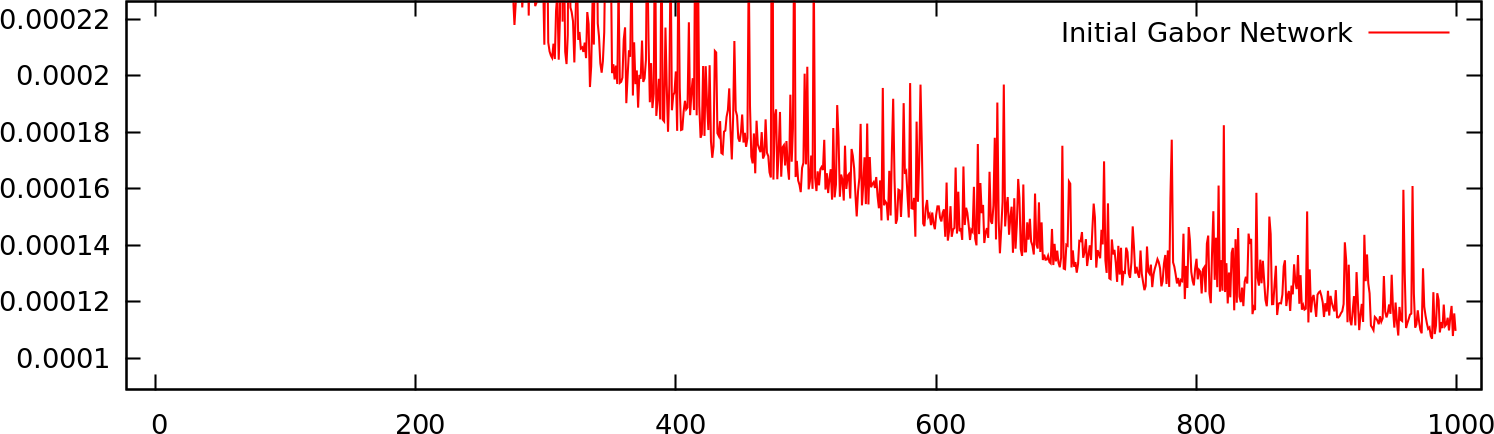
\includegraphics[width=\textwidth]{images/results/gabor_initial_network.png}
	\caption{Training error of the initial Gabor network for 1,000 epochs}
	\label{fig:gabor_initial_network}
\end{figure}

\begin{table}[h!]
\centering
\footnotesize
\begin{tabular}{|l|l|l|l|l|}
	\hline
		\textbf{Setup} & \textbf{Training error} & \textbf{Training error (pixels)} & \textbf{Test error} & \textbf{Test error (pixels)}\\
	\hline
		1,000	& 0.0001100461%9286889145
				& 1.3427571723%74781
				& 0.0004099451%7442226796
				& 2.5916291667%08547
				\\
%	\hline
%		1,500 	& 0.0000910564%24015354854
%				& 1.2214206691%666774
%				& 0.0004021702%247910016
%				& 2.5669353250%47316
%				\\
	\hline
	\end{tabular}
	\normalsize
	\caption{Errors for the inital network after 1,000 epochs}
	\label{tab:gabor_errors_initial_network}
\end{table}


Both error values are better than all the error values of the first regarded conventionally trained \acp{CNN} above in chapter \ref{subsubsec:color_gray_learningrate}. The test error is even the best test error achieved so far, but nevertheless a lot more networks were examined for the purpose of finding a network, which produces an even better test error.

\subsubsection{Increasing the Resolution}

The research about the conventionally trained \acp{CNN} has shown that increasing the resolution of the input images slightly improved the performance of the network. Therefore it makes sense to increase the resolution of the input images from $96\times128$ to $120\times160$ also for the Gabor wavelet based networks. Figure \ref{fig:gabor_absatan2_96_vs_120} shows the plot for the network with the small input image resolution and the network with the larger input image resolution.

\begin{figure}[h!]
	\centering
	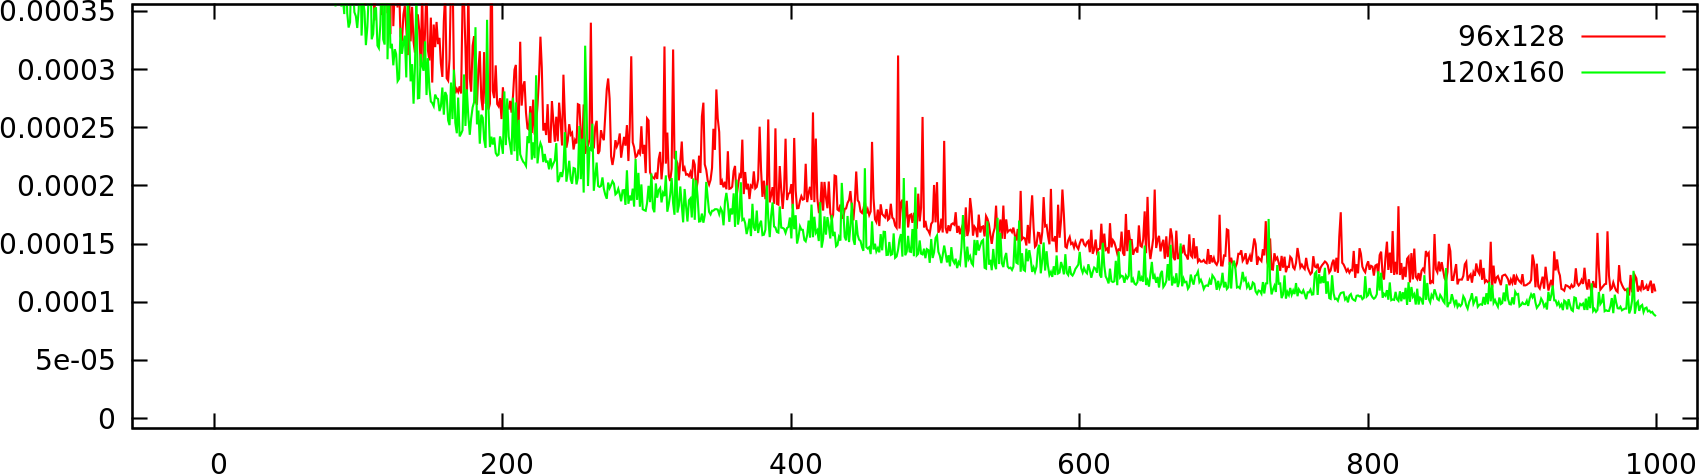
\includegraphics[width=\textwidth]{images/results/gabor_absatan2_96_vs_120.png}
	\caption{Training error for resolution $96\times128$ and $120\times160$}
	\label{fig:gabor_absatan2_96_vs_120}
\end{figure}

As already observed for the \acp{CNN} examined above, the network with the larger input maps produces a lower training error than the network with the smaller input maps. Table \ref{tab:gabor_errors_96_vs_120} contains the training and test errors of both networks after 1,000 epochs.

\begin{table}[h!]
\centering
\footnotesize
\begin{tabular}{|l|l|l|l|l|}
	\hline
		\textbf{Setup} & \textbf{Training error} & \textbf{Training error (pixels)} & \textbf{Test error} & \textbf{Test error (pixels)}\\
	\hline
		$96\times128$	& 0.0001100461%9286889145
						& 1.3427571723%74781
						& 0.0004099451%7442226796
						& 2.5916291667%08547
						\\
	\hline
		$120\times160$ 	& 0.0000886053%969184021
						& 1.5060870363%664558
						& 0.0003811093%5314900139
						& 3.1235235617%191104
						\\
	\hline
	\end{tabular}
	\normalsize
	\caption{Errors for input images of size $96\times128$ and $120\times160$}
	\label{tab:gabor_errors_96_vs_120}
\end{table}


Table \ref{tab:gabor_errors_480_96_vs_120} shows the same errors normalized to the original image resolution of $480\times640$ pixels. The difference between the error of the network with input maps of size $96\times128$ and the error of the network with input maps of size $120\times160$ is not overwhelmingly huge, but sufficiently large to use the increased resolution for all following networks.

\begin{table}[h!]
\centering
\footnotesize
\begin{tabular}{|l|l|l|}
	\hline
		\textbf{Setup} & \textbf{Upscaled Training Error} & \textbf{Upscaled Test Error}\\
	\hline
		$96\times128$	& 6.713785862
						& 12.95814583
						\\
	\hline
		$120\times160$ 	& 6.024348145
						& 12,49409425
						\\
	\hline
	\end{tabular}
	\normalsize
	\caption{Upscaled errors for input images of size $96\times128$ and $120\times160$}
	\label{tab:gabor_errors_480_96_vs_120}
\end{table}


Table \ref{tab:gabor_params_120} contains the usual information about the network. The structure of the network is still the same as the one depicted in figure \myref{fig:gabor_structure_initial_network}.

\begin{table}[h!]
	\footnotesize
	\centering
	\begin{tabular}{ll}
	\hline
		\textbf{Parameter} & \textbf{Value}\\
	\hline
	\hline
		\textbf{Resolution} & $3 \times 120\times160$\\
		\textbf{Learning rate} & 0.1\\
		\textbf{Batch size} & 4\\
		\textbf{Epochs} & 1000\\
		\textbf{Trainable parameters} & 116,672,002\\
		\textbf{Execution time} & 168,483s\\
		\textbf{GPU} & GeForce GTX 780\\
	\hline
	\end{tabular}
	\caption{Parameters for the Gabor network with $120\times160$ input maps}
	\label{tab:gabor_params_120}
\end{table}


The table reveals that it took 168,483 seconds to train the network for 1,000 epochs. This is almost twice as much time as was required to train the network with the smaller input maps. This finding is completely logical, because also the number of free parameters (116,672,002) is almost twice as large as in the previously considered network (65,369,602).

\subsubsection{Omitting Color Information}

Since using images with three color channels as input for such a large network is quite costly in terms of computation time, a network with only one gray-value input map was compared to the network with three input maps. Reducing the number of input maps from 3 to 1 does not change the number of trainable parameters, because every layer except the Gabor layer remain unchanged. Since the weights in the Gabor layer are fixed and do not get updated, the number of trainable parameters remains the same. Nonetheless, the computation time is reduced from 168,483s to 102,147s, because the number of the costly convolutions in the Gabor layer is reduced from 240 to 80 for each input image.

Figure \ref{fig:gabor_absatan2_color_vs_gray} opposes the plots of the training errors for the network with \ac{RGB} input images and the network with gray-value input images. As already seen for the \acp{CNN} without Gabor wavelets above, color information improves the performance of the network.

\begin{figure}[h!]
	\centering
	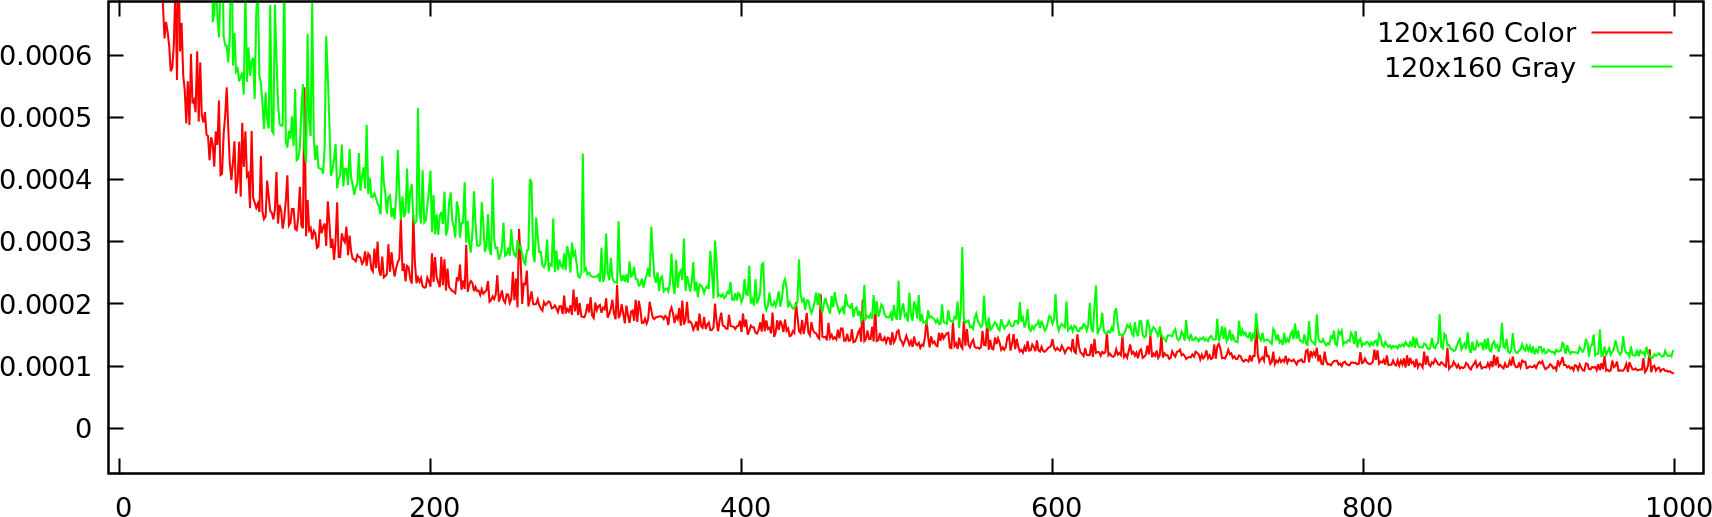
\includegraphics[width=\textwidth]{images/results/gabor_absatan2_color_vs_gray.png}
	\caption{Training error for the color network and the gray-value network}
	\label{fig:gabor_absatan2_color_vs_gray}
\end{figure}

Again, this assumption is supported by the error values after the last epoch of the training process, which can be found in table \ref{tab:gabor_errors_color_vs_gray}. Even though the error values indicate that the difference between the error values is not negligible, the networks, which are still to be considered in this thesis, refrain from exploiting the color information for the benefit of shorter training times.

\begin{table}[h!]
\centering
\footnotesize
\begin{tabular}{|l|l|l|l|l|}
	\hline
		\textbf{Setup} & \textbf{Training error} & \textbf{Training error (pixels)} & \textbf{Test error} & \textbf{Test error (pixels)}\\
	\hline
		color 	& 0.0000886053%969184021
				& 1.5060870363%664558
				& 0.0003811093%5314900139
				& 3.1235235617%191104
				\\
	\hline
		gray	& 0.0001238262%047248818
				& 1.7804355761%883028
				& 0.0005460486%0983845668
				& 3.7388292835%945975
				\\
	\hline
	\end{tabular}
	\normalsize
	\caption{Errors for RGB images and gray-value images}
	\label{tab:gabor_errors_color_vs_gray}
\end{table}


\subsubsection{Changing the Parameters of the On-Line Distortions}
\label{subsubsec:newparameters}

Since the \ac{MUCT} data set contains a certain amount of images, which show persons with rather uncommon head postures, it has been decided to change the parameters of the on-line distortions in such a way that some of the images, which show usual head postures, are transformed so that they resemble those images, which show uncommon head postures. In order to achieve this, the images are no longer shifted by 10\% of the image's height or width, respectively, but by 20\%. Additionally, the interval of the scale factors was narrowed from $[0.9,1.1]$ to $[0.95,1.05]$. The rotation angles are still drawn from a uniform distribution in the interval $[-5,5]$. Table \ref{fig:gabor_absatan2_np_vs_op} shows the training and the test error of the network with the new parameters and of the network with the old parameters after 1,000 epochs. Training the network with the new parameters took 102,009 seconds.
\begin{table}[h!]
\centering
\footnotesize
\begin{tabular}{|l|l|l|l|l|}
	\hline
		\textbf{Setup} & \textbf{Training error} & \textbf{Training error (pixels)} & \textbf{Test error} & \textbf{Test error (pixels)}\\
	\hline
		old parameters	& 0.0001238262%047248818
						& 1.7804355761%883028
						& 0.0005460486%0983845668
						& 3.7388292835%945975
						\\
	\hline
		new parameters 	& 0.0001264428%4201810042
						& 1.7991488975%800116
						& 0.0006120212%749442589
						& 3.9582501990%87095
						\\
	\hline
	\end{tabular}
	\normalsize
	\caption{Errors for the new and the old on-line distortion parameters}
	\label{tab:gabor_errors_np_vs_op}
\end{table}


The training error of both networks is almost equal. Despite the unfavorable fact that the network with the old parameters produces a noticeable smaller test error than the network with the new parameters, all following networks were trained with the new parameter set. This should not make a too big difference, because the curves of the training errors of both networks shown in figure \ref{fig:gabor_absatan2_np_vs_op} are very similar, at least after the first 500 epochs.

\begin{figure}[h!]
	\centering
	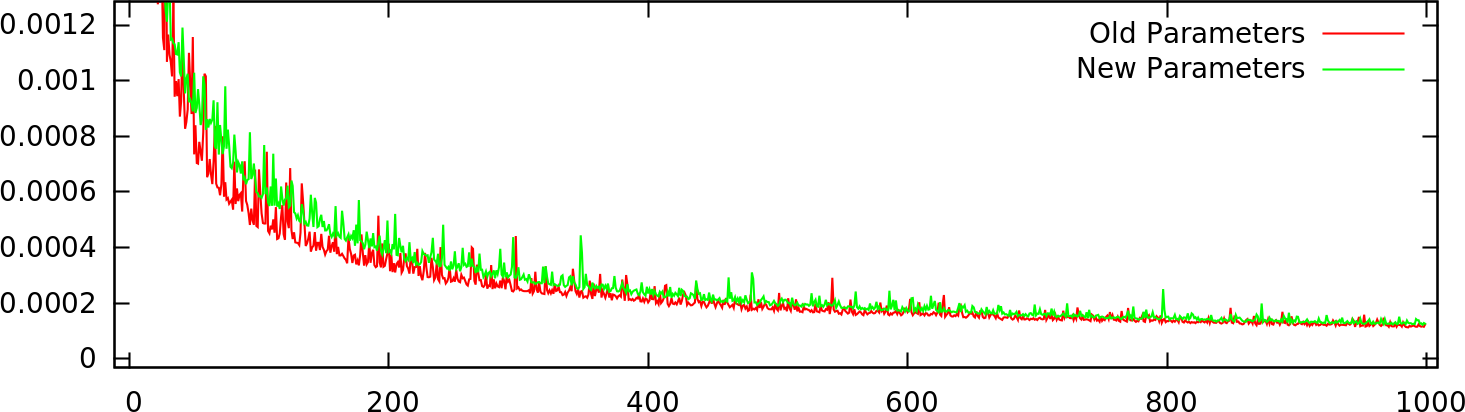
\includegraphics[width=\textwidth]{images/results/gabor_absatan2_np_vs_op.png}
	\caption{Training error for new and old on-line distortion parameters}
	\label{fig:gabor_absatan2_np_vs_op}
\end{figure}

\subsubsection{Linear Activation Function and Dropout}

The next experiment treats the question whether the \ac{ReLU} is a good choice as activation function after the convolutions in the Gabor layer, because it is not thoroughly clear whether the behavior of the \ac{ReLU}, i.e. setting all negative values to $0$, is beneficial or potentially problematic for the given regression task. Hence, the \ac{ReLU} in the Gabor layer was replaced by a simple linear activation function. This is best visualized by mentally replacing the symbolic \ac{ReLU} activation functions in the small squares in figure \myref{fig:merge_abs_atan2} with straight lines with slope $1$.\\
The plot in figure \ref{fig:gabor_absatan2_linear}, which shows the training error of the network with the \ac{ReLU} and the training error of the network with the linear activation function, reveals that both networks perform almost equally well, even though the \ac{ReLU}-network functions a little bit better.

\begin{figure}[h!]
	\centering
	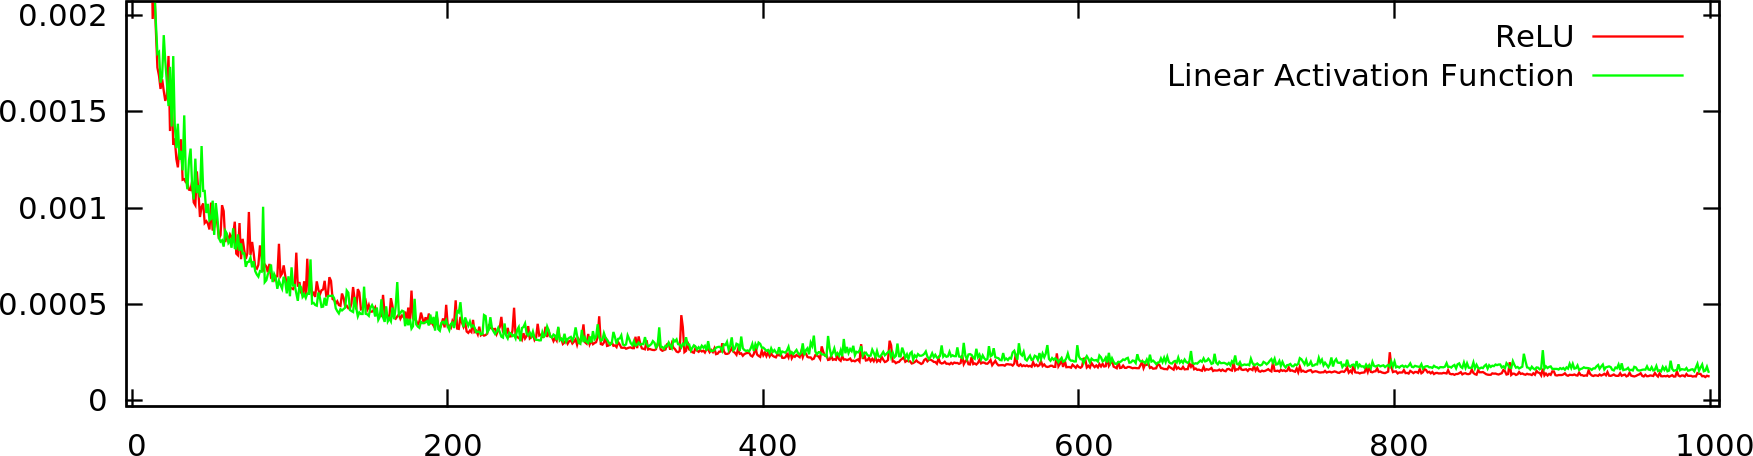
\includegraphics[width=\textwidth]{images/results/gabor_absatan2_linear.png}
	\caption{Training error for ReLU and linear activation function}
	\label{fig:gabor_absatan2_linear}
\end{figure}
Since calculating the gradient of a smooth linear function should be computationally less costly than computing the gradient of a linear function with a case distinction (smaller or larger than $0$?), one would expect that the network with the linear activation function should be executed in less time than the network with the \ac{ReLU} activation function. Contrary to these expectations, the execution time of the network with the linear activation function (104,047s) turned out to be even longer than the computation time required by the \ac{ReLU} network (102,009s). A possible reason for this observation could be that the server, on which the networks were trained, may have been executing another program simultaneously. Another cause may be internal implementation issues of Keras.\\
The observation that the \ac{ReLU}-network produces a slightly smaller training error is confirmed by the error values in table \ref{tab:gabor_errors_relu_vs_linear}. However, since the test error after the 1,000th epoch is smaller for the network with the linear activation function, two more networks with the linear activation function were constructed.
\begin{table}[h!]
\centering
\footnotesize
\begin{tabular}{|l|l|l|l|l|}
	\hline
		\textbf{Setup} & \textbf{Training error} & \textbf{Training error (pixels)} & \textbf{Test error} & \textbf{Test error (pixels)}\\
	\hline
		ReLU 	& 0.0001264428%4201810042
				& 1.7991488975%800116
				& 0.0006120212%749442589
				& 3.9582501990%87095
				\\
	\hline
		Linear	& 0.0001501458%6131201213
				& 1.9605443248%209184
				& 0.0005448454%9607827022
				& 3.7347081143%783805
				\\
	\hline
	\end{tabular}
	\normalsize
	\caption{Errors for the ReLU and the linear activation function}
	\label{tab:gabor_errors_relu_vs_linear}
\end{table}

These networks use a dropout layer after the Gabor layer in order to achieve sparseness by deactivating a randomly chosen subset of the connections between two layers instead of letting through only positive values like the \ac{ReLU}. This way, the systematic refusal of information by the \ac{ReLU} should be avoided. The green curve in figure \ref{fig:gabor_absatan2_linear_dropout05} shows the training error for the network with the linear activation function but without a dropout layer. The network, whose training error is represented by the blue curve, was equipped with a dropout layer, which omitted 30\% of the connections between the Gabor layer and the convolutional layer. The third network (violet curve) used a dropout layer, which ignored 50\% of the connections during each weight update step.
\begin{figure}[h!]
	\centering
	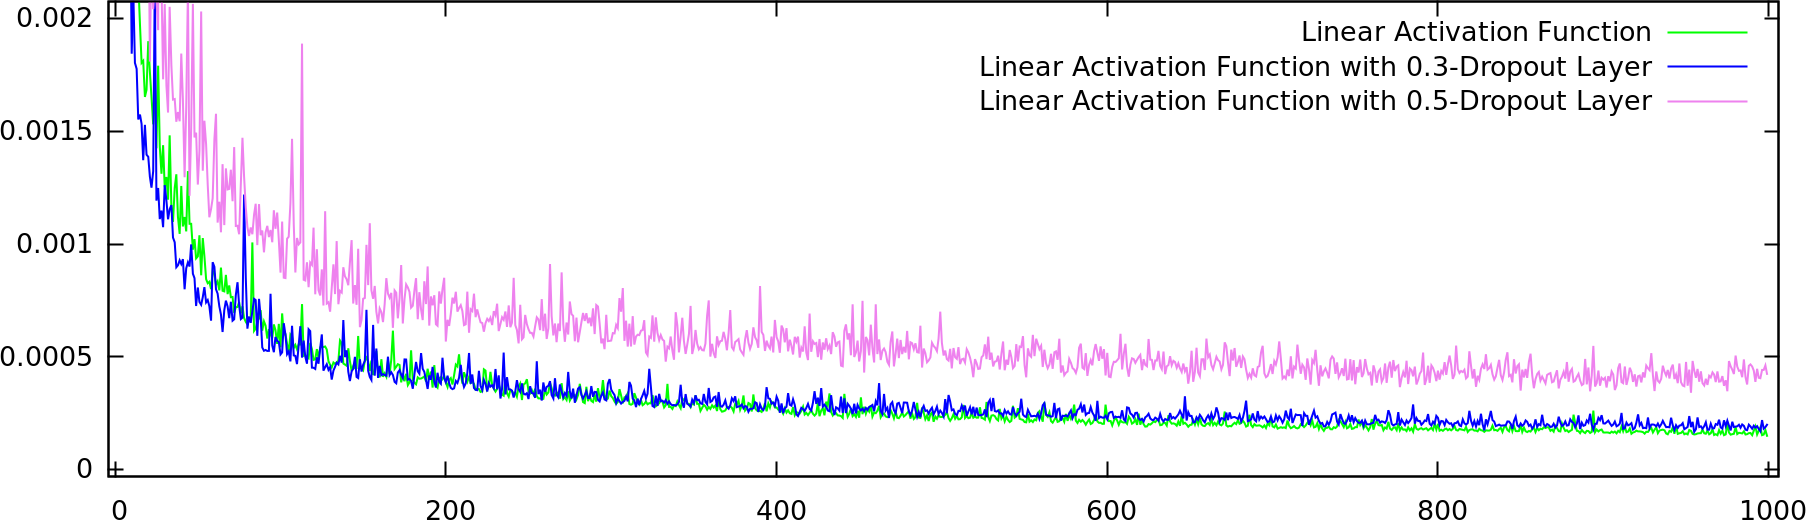
\includegraphics[width=\textwidth]{images/results/gabor_absatan2_linear_dropout05.png}
	\caption{Training error with and without dropout}
	\label{fig:gabor_absatan2_linear_dropout05}
\end{figure}

While a dropout rate of 50\% is obviously too high, a rate of 30\% seems to have almost no effect on the training error.
\begin{table}[h!]
\centering
\footnotesize
\begin{tabular}{|l|l|l|l|l|}
	\hline
		\textbf{Setup} & \textbf{Training error} & \textbf{Training error (pixels)} & \textbf{Test error} & \textbf{Test error (pixels)}\\
	\hline
		no dropout		& 0.0001501458%6131201213
						& 1.9605443248%209184
						& 0.0005448454%9607827022
						& 3.7347081143%783805
						\\
	\hline
		0.3 dropout 	& 0.0001987915%9818321658
						& 2.2558955901%127926
						& 0.0005090703%4532421695
						& 3.6100139667%73529
						\\
	\hline
		0.5 dropout 	& 0.0004244664%2619407908
						& 3.2964132796%978634
						& 0.0006743826%1828578971
						& 4,155020461 %
						\\
	\hline
	\end{tabular}
	\normalsize
	\caption{Errors with and without dropout}
	\label{tab:gabor_errors_dropout}
\end{table}

Calculating the training error and the test error after the 1000th epoch support these assumptions. The corresponding values can be found in table \ref{tab:gabor_errors_dropout}. The training error of the network with dropout rate 0.3 is slightly larger than the training error of the network without any dropout layer. However, the test error is a little bit smaller for the network with dropout layer. Both the training and the test error of the network with dropout rate 0.5 are much larger than the corresponding errors of the other two networks. Even worse, the network with the larger dropout rate did not only compute a worse result but took more computation time (105,779s) than the network with dropout rate 0.3 (104,233s). Since neither using a linear activation function nor incorporating a dropout layer into the network improved the network's performance, all upcoming networks will use the \ac{ReLU} activation function and will have no dropout layer. Nonetheless, the structure of this kind of network is illustrated by figure \ref{fig:gabor_structure_dropout}.
\begin{figure}[h!]
	\scriptsize
	\centering
	\begin{tabular}{|c|}
	\hline
		\textbf{Gabor Layer}\\
		3 input maps, 80 output maps, absolute value and phase, Linear\\
		filter sizes: $27 \times 27$, $31 \times 31$, $39 \times 39$, $47 \times 47$ and $55 \times 55$\\
	\hline
		\textbf{Dropout Layer}\\
		dropout rate 0.5\\
	\hline
		\textbf{Convolutional Layer}\\
		80 input maps, 32 output maps, filter size $3\times3$, Glorot normal initialization, \ac{ReLU}\\
	\hline
		\textbf{Fully Connected Layer}\\
		300 neurons, Glorot normal initialization, sigmoid\\
	\hline
		\textbf{Fully Connected Layer}\\
		200 neurons, Glorot normal initialization, sigmoid\\
	\hline
		\textbf{Output Layer}\\
		30 neurons, Glorot normal initialization\\
	\hline
	\end{tabular}
	\caption{Structure of a Gabor network with dropout layer}
	\label{fig:gabor_structure_dropout}
\end{figure}
	

\subsubsection{Increasing the Size of the Convolutional Layer}

Since increasing the size of the filters in the convolutional layers improved the performance of the \acp{CNN} without Gabor wavelets, the size of the filters of the convolutional layer which succeeds the Gabor layer was increased from $3\times3$ to $7\times7$. 
\begin{figure}[h!]
	\centering
	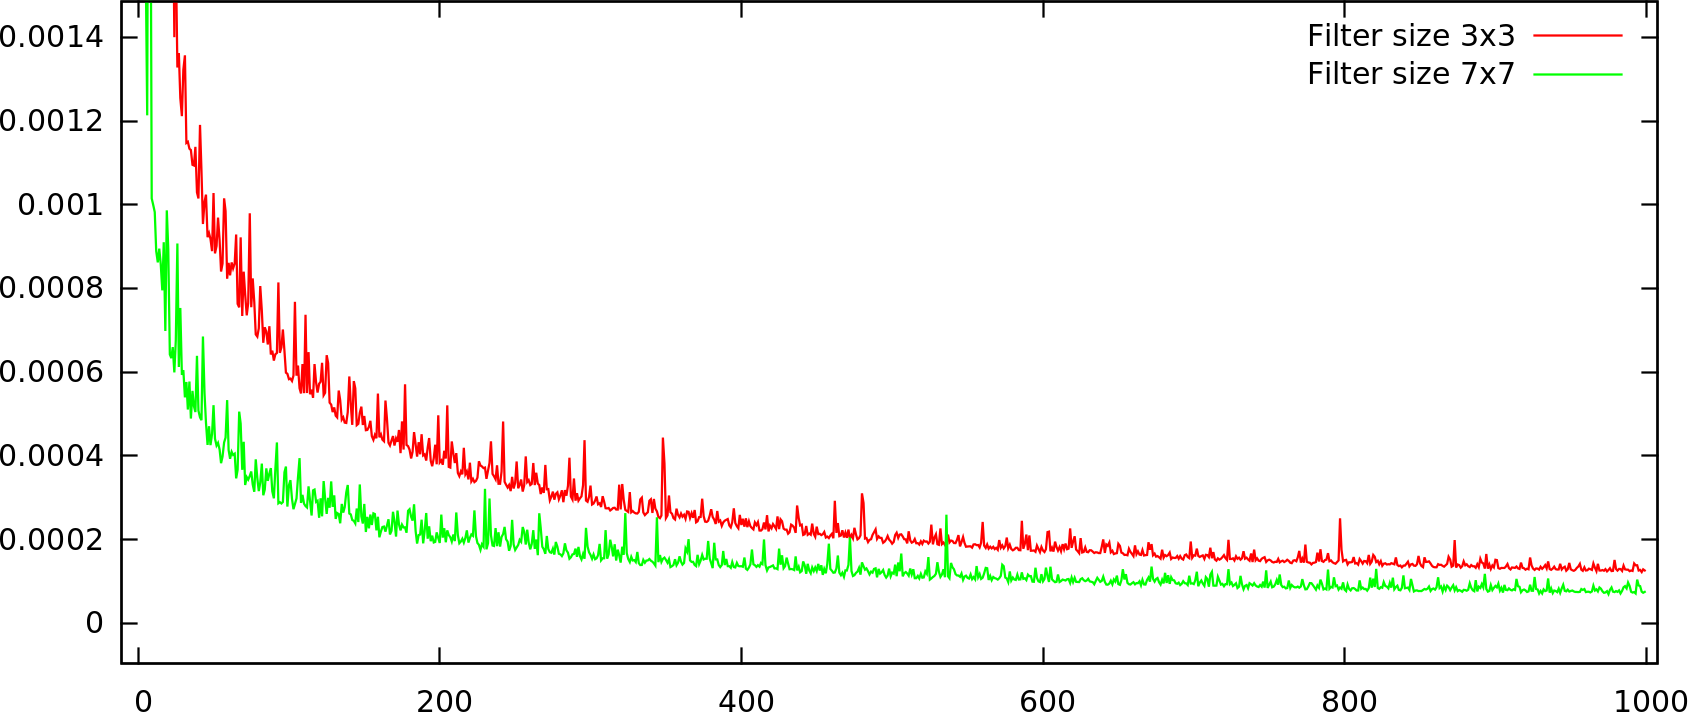
\includegraphics[width=\textwidth]{images/results/gabor_absatan2_largerconv.png}
	\caption{Training error with filter size $3\times3$ and filter size $7\times7$}
	\label{fig:gabor_absatan2_largerconv}
\end{figure}
Figure \ref{fig:gabor_absatan2_largerconv} opposes the curves of the training errors of the network with filter size $3\times3$ and the network with filter size $7\times7$. As the green line dominates the red line over all 1,000 epochs, the larger filters have a clearly positive impact on the success of the training process. 
\begin{table}[h!]
\centering
\footnotesize
\begin{tabular}{|l|l|l|l|l|}
	\hline
		\textbf{Setup} & \textbf{Training error} & \textbf{Training error (pixels)} & \textbf{Test error} & \textbf{Test error (pixels)}\\
	\hline
		3x3 & 0.0001264428%4201810042
			& 1.7991488975%800116
			& 0.0006120212%749442589
			& 3.9582501990%87095
			\\
	\hline
		7x7	& 0.0000753599%85959604279
			& 1.3889620731%200218
			& 0.0003950733%1637073795
			& 3.1802322083%600894
			\\
	\hline
	\end{tabular}
	\normalsize
	\caption{Training errors for filter size $3\times3$ and $7\times7$}
	\label{tab:gabor_errors_3x3_vs_7x7}
\end{table}

The error values in table \ref{tab:gabor_errors_3x3_vs_7x7} show that the performance of the network improved not only on the training data but also on the test data. The test error is even the best value since the one of the last network which uses color information. Since larger filters are beneficial for \acp{CNN} with and without Gabor wavelets, they seem to be advantageous in general. Chapter \myref{subsubsec:newparameters} and table \ref{tab:gabor_params_largerconv} reveal that the execution time increased from 102,009 seconds to 112,543 seconds. As the performance improvement is notable, the increased amount of required execution time should not preponderate.

\begin{table}[h!]
	\footnotesize
	\centering
	\begin{tabular}{ll}
	\hline
		\textbf{Parameter} & \textbf{Value}\\
	\hline
	\hline
		\textbf{Resolution} & $1 \times 120\times160$\\
		\textbf{Learning rate} & 0.1\\
		\textbf{Batch size} & 4\\
		\textbf{Epochs} & 1000\\
		\textbf{Trainable parameters} & 108,326,402\\
		\textbf{Execution time} & 112,543s\\
		\textbf{GPU} & GeForce GTX 780\\
	\hline
	\end{tabular}
	\caption{Parameters for the Gabor network with filter size $7\times7$}
	\label{tab:gabor_params_largerconv}
\end{table}


Finally, figure \ref{fig:gabor_structure_largerconv} compactly illustrates the structure of the current best network.

\begin{figure}[h!]
	\scriptsize
	\centering
	\begin{tabular}{|c|}
	\hline
		\textbf{Gabor Layer}\\
		3 input maps, 80 output maps, absolute value and phase, ReLU\\
		filter sizes: $27 \times 27$, $31 \times 31$, $39 \times 39$, $47 \times 47$ and $55 \times 55$\\
	\hline
		\textbf{Convolutional Layer}\\
		80 input maps, 32 output maps, filter size $7\times7$, Glorot normal initialization, \ac{ReLU}\\
	\hline
		\textbf{Fully Connected Layer}\\
		300 neurons, Glorot normal initialization, sigmoid\\
	\hline
		\textbf{Fully Connected Layer}\\
		200 neurons, Glorot normal initialization, sigmoid\\
	\hline
		\textbf{Output Layer}\\
		30 neurons, Glorot normal initialization\\
	\hline
	\end{tabular}
	\caption{Structure of the Gabor network with filter size $7\times7$}
	\label{fig:gabor_structure_largerconv}
\end{figure}


\subsubsection{Using Two Large Convolutional Layers}

The last network whose Gabor layer creates 80 output maps by merging the Gabor responses with both introduced operations, uses two convolutional layers instead of a single one. Since increasing the convolutional layer's size was beneficial to the network's prediction ability, the filters of both convolutional layers are even larger than those of the previously regarded network. As can be seen in figure \ref{fig:gabor_structure_2cl}, the first convolutional layer after the Gabor layer has filters of size $15\times15$ and, just as like the previously used convolutional layers, produces 32 output maps.
\begin{figure}[h!]
	\scriptsize
	\centering
	\begin{tabular}{|c|}
	\hline
		\textbf{Gabor Layer}\\
		3 input maps, 80 output maps, absolute value and phase, ReLU\\
		filter sizes: $27 \times 27$, $31 \times 31$, $39 \times 39$, $47 \times 47$ and $55 \times 55$\\
	\hline
		\textbf{Convolutional Layer}\\
		80 input maps, 32 output maps, filter size $15\times15$, Glorot normal initialization, \ac{ReLU}\\
	\hline
		\textbf{Convolutional Layer}\\
		32 input maps, 24 output maps, filter size $9\times9$, Glorot normal initialization, \ac{ReLU}\\
	\hline
		\textbf{Fully Connected Layer}\\
		300 neurons, Glorot normal initialization, sigmoid\\
	\hline
		\textbf{Fully Connected Layer}\\
		200 neurons, Glorot normal initialization, sigmoid\\
	\hline
		\textbf{Output Layer}\\
		30 neurons, Glorot normal initialization\\
	\hline
	\end{tabular}
	\caption{Structure of the Gabor network with two convolutioal layers}
	\label{fig:gabor_structure_2cl}
\end{figure}

The second convolutional layer, however, has filters of size $9\times9$ and creates 24 output maps. Thus, there are $24\cdot32=768$ filters between both convolutional layers.
\begin{figure}[h!]
	\centering
	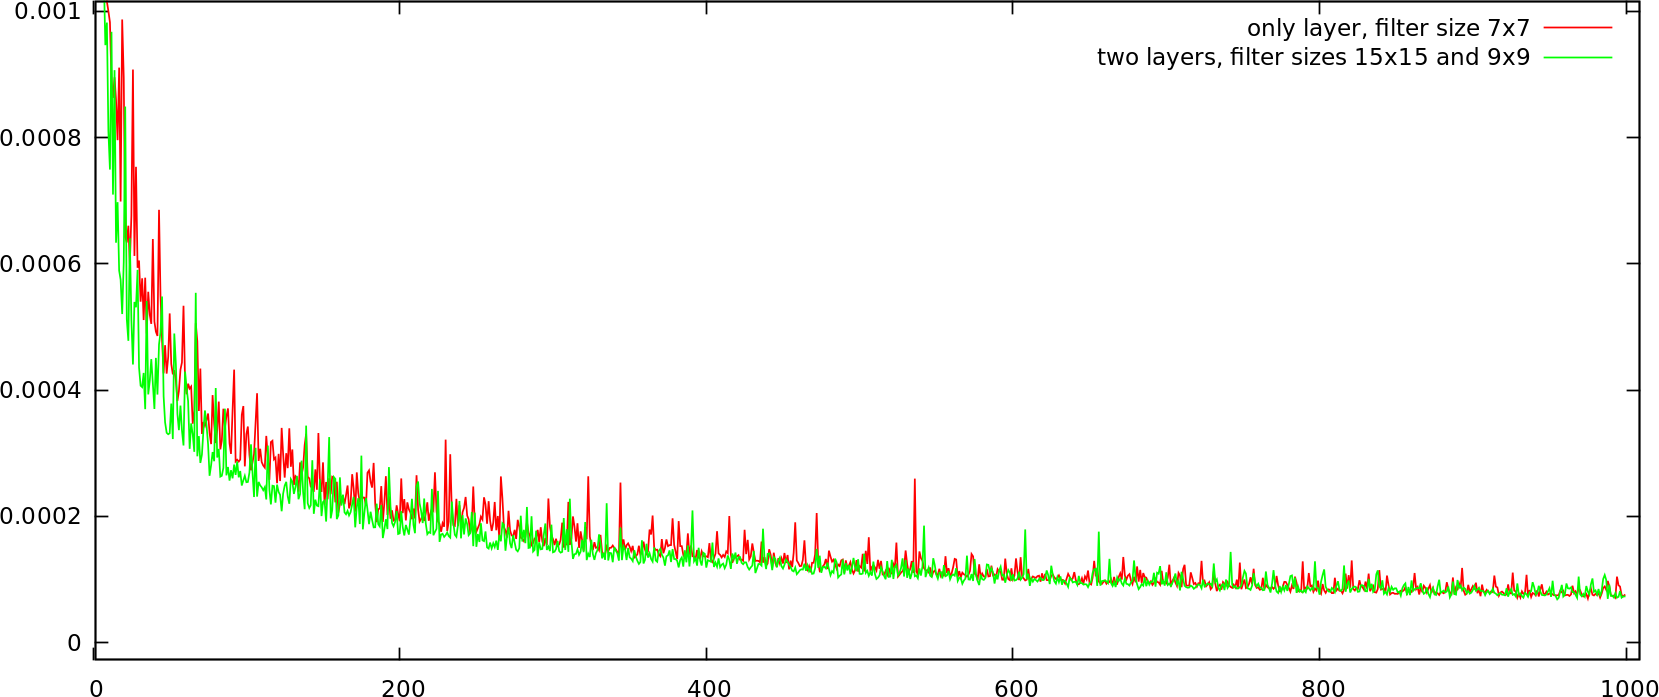
\includegraphics[width=\textwidth]{images/results/gabor_absatan2_2cl.png}
	\caption{Training error with one and with two convolutional layers}
	\label{fig:gabor_absatan2_2cl}
\end{figure}
Figure \ref{fig:gabor_absatan2_2cl} evinces that the network with two convolutional layers initially dominates the network with only one layer. Later on, both networks perform virtually equally well on the training data. Table \ref{tab:gabor_errors_2cl}

\begin{table}[h!]
\centering
\footnotesize
\begin{tabular}{|l|l|l|l|l|}
	\hline
		\textbf{Setup} & \textbf{Training error} & \textbf{Training error (pixels)} & \textbf{Test error} & \textbf{Test error (pixels)}\\
	\hline
		one layer	& 0.0000753599%85959604279
					& 1.3889620731%200218
					& 0.0003950733%1637073795
					& 3.1802322083%600894
					\\
	\hline
		two layers	& 0.0000731925%41588294461
					& 1.3688422351%24391
					& 0.0003165762%6308453598
					& 2.8468144187%78316
					\\
	\hline
	\end{tabular}
	\normalsize
	\caption{Training errors with one and with two convolutional layers}
	\label{tab:gabor_errors_2cl}
\end{table}



\subsubsection{One Merging Operation instead of Two}

\textcolor{white}{asdfas}%TODO Remove me
\newpage

\subsection*{Provisional Results Overview}
asdf
% gabor_lr0.1_absatan2_cuda01
% gabor_lr0.1_absatan2_hd_cuda01
% gabor_lr0.1_absatan2_hd_gray_cuda01
% gabor_lr0.1_absatan2_hd_gray_np_cuda01
% gabor_lr0.1_absatan2_hd_gray_linear_cuda01
% gabor_lr0.1_absatan2_hd_gray_linear_dropout_cuda01
% gabor_lr0.1_absatan2_hd_gray_linear_dropout05_cuda01
% gabor_lr0.1_absatan2_hd_gray_noconv_cuda01
% gabor_lr0.1_absatan2_hd_gray_largerconv_cuda01
% gabor_lr0.1_absatan2_hd_gray_2cl_cuda01
% gabor_lr0.1_abs_hd_gray_2cl_cuda01
% gabor_lr0.1_atan2_hd_gray_2cl_cuda01

\tiny
\begin{tabular}{|l|l|l|l|l|}
\hline
	\textbf{Setup} & \textbf{Training error} & \textbf{Training error (pixels)} & \textbf{Test error} & \textbf{Test error (pixels)}\\
\hline
	2cl atan2 2000 & 5.0980641299870449e-05 & 1.1424116671658617 & 0.00043121594174221544 & 3.322518338339266\\
\hline
	2cl atan2 1500 & 6.8641028017271848e-05 & 1.3255980979324613 & 0.00045517455199553872 & 3.4135712283597934\\
\hline
	2cl atan2 1000 & 8.3859986954317288e-05 & 1.4652015786336439 & 0.00046992166700326565 & 3.468428271607127\\
%\hline
%	2cl & 7.3192541588294461e-05 & 1.368842235124391 & 0.00031657626308453598 & 2.846814418778316\\
%\hline
%	largerconv & 7.5359985959604279e-05 & 1.3889620731200218 & 0.00039507331637073795 & 3.1802322083600894\\
%\hline %dropped from considerations due to lacking reproducability
%	noconv & 0.00017174116032 & 2.096800826 & TBD & TBD\\
%\hline
%	lin. dropout05 & 0.00042446642619407908 & 3.2964132796978634 & 0.00067438261828578971 & 0.00067438261828578971\\
%\hline
%	lin. dropout & 0.00019879159818321658 & 2.2558955901127926 & 0.00050907034532421695 & 3.610013966773529\\
%\hline
%	linear & 0.00015014586131201213 & 1.9605443248209184 & 0.00054484549607827022 & 3.7347081143783805\\
%\hline
%	np & 0.00012644284201810042 & 1.7991488975800116 & 0.0006120212749442589 & 3.958250199087095\\
%\hline
%	absatan2\_hd\_gray & 0.0001238262047248818 & 1.7804355761883028 & 0.00054604860983845668 & 3.7388292835945975\\
\hline
%	absatan2\_hd & 8.86053969184021e-05 & 1.5060870363664558 & 0.00038110935314900139 & 3.1235235617191104\\
%\hline
%	absatan2 (color) & 0.00011004619286889145 & 1.342757172374781 & 0.00040994517442226796 & 2.591629166708547\\
%\hline
\end{tabular}
\normalsize

asdf

\begin{figure}[htbp]
	\centering
	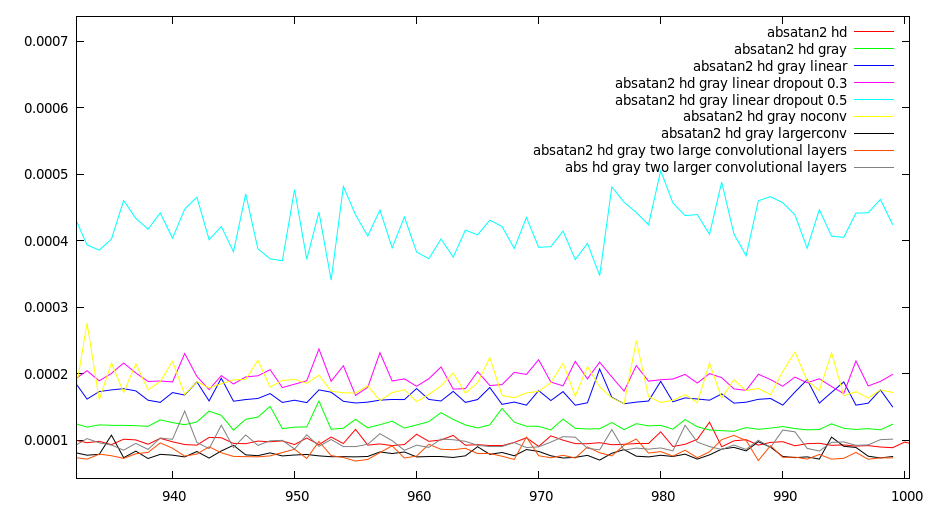
\includegraphics[width=0.9\textwidth]{results/absatan2_and_abs_1.png}
	\caption{Results for all absatan2 and abs networks after 1,000 epochs}
	\label{fig:absatan2_results}
\end{figure}

\begin{figure}[htbp]
	\centering
	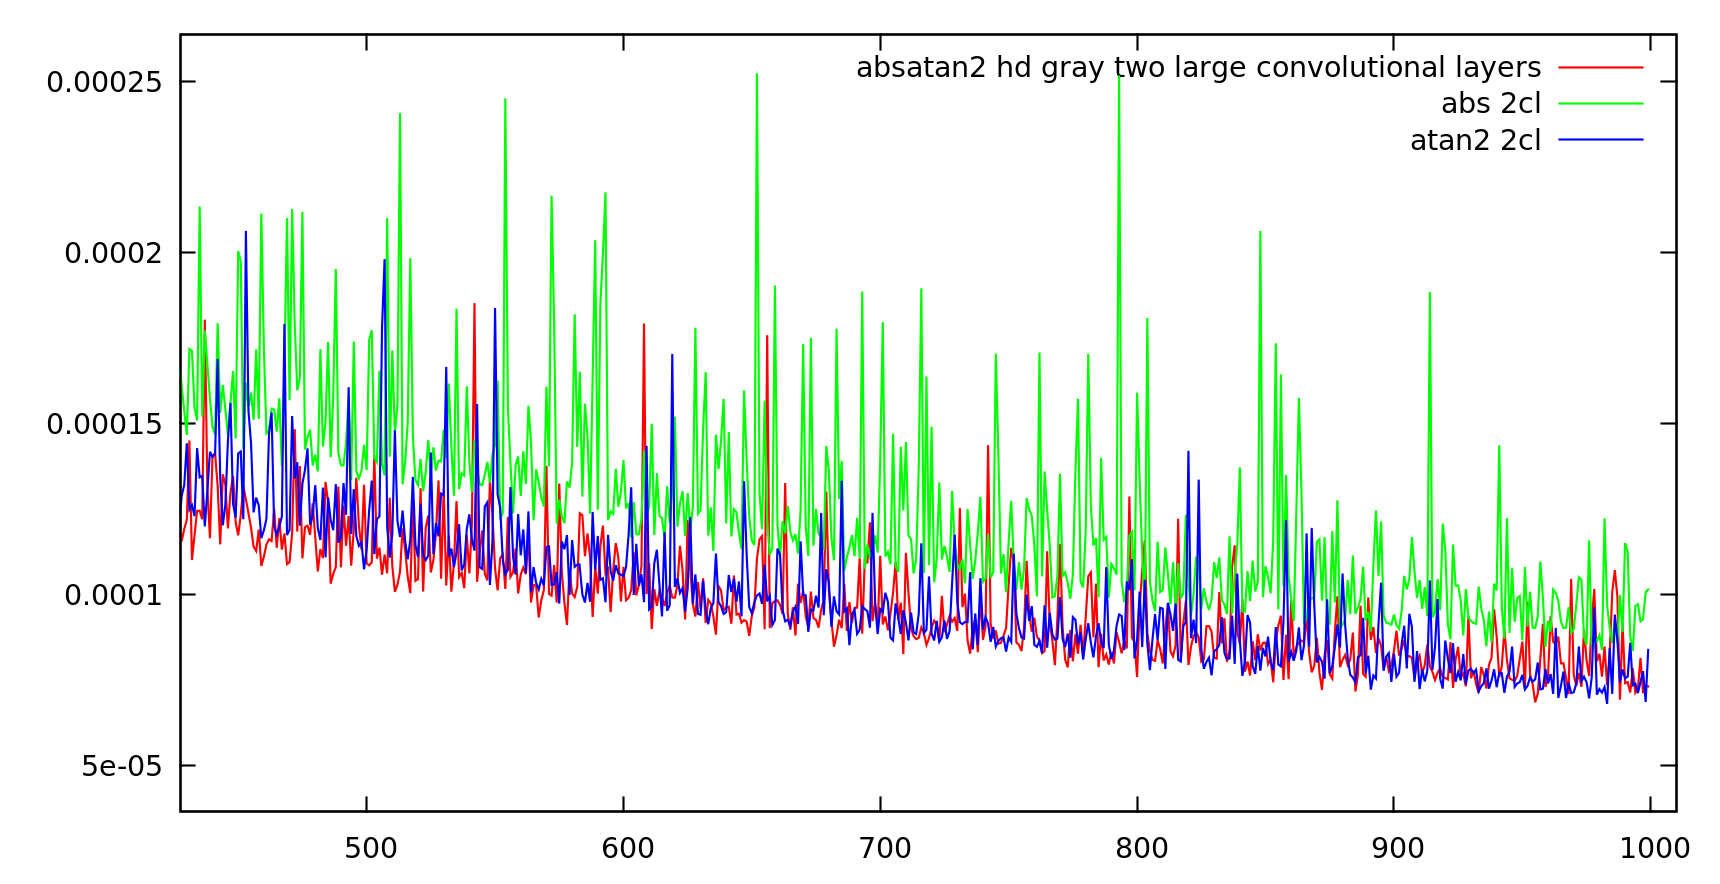
\includegraphics[width=0.9\textwidth]{results/gabor_absatan2_vs_atan2_vs_abs.png}
	\caption{Absatan2 vs atan2 vs abs after 1,000 epochs}
	\label{fig:gabor_absatan2_vs_atan2_vs_abs}
\end{figure}


\newpage

%%%%%%%%%%%%%%%%%%%%%%%%%%%%%%%%%%%%%%%%%%%%%%%%%%%%%%%%%%%%%%%%%%%%%%%%%%%%%%%%%%%%%%%%%%%%%%%%%%%%%%%%%
%%%%%%%%%%%%%%%%%%%%%%%%%%%%%%%%%%%%%%%%%%%%%%%%%%%%%%%%%%%%%%%%%%%%%%%%%%%%%%%%%%%%%%%%%%%%%%%%%%%%%%%%%
%									CONCLUSION CHAPTER BEGINS HERE										%
%%%%%%%%%%%%%%%%%%%%%%%%%%%%%%%%%%%%%%%%%%%%%%%%%%%%%%%%%%%%%%%%%%%%%%%%%%%%%%%%%%%%%%%%%%%%%%%%%%%%%%%%%
%%%%%%%%%%%%%%%%%%%%%%%%%%%%%%%%%%%%%%%%%%%%%%%%%%%%%%%%%%%%%%%%%%%%%%%%%%%%%%%%%%%%%%%%%%%%%%%%%%%%%%%%%

\section{Conclusion}
\label{sec:conclusion}

Conventionally trained \acp{CNN} are able to make the training error very small but produce high test errors. Gabor wavelet based networks do not produce so small training errors but better test errors.

\newpage

%%%%%%%%%%%%%%%%%%%%%%%%%%%%%%%%%%%%%%%%%%%%%%%%%%%%%%%%%%%%%%%%%%%%%%%%%%%%%%%%%%%%%%%%%%%%%%%%%%%%%%%%%
%%%%%%%%%%%%%%%%%%%%%%%%%%%%%%%%%%%%%%%%%%%%%%%%%%%%%%%%%%%%%%%%%%%%%%%%%%%%%%%%%%%%%%%%%%%%%%%%%%%%%%%%%
%										APPENDIX BEGINS HERE											%
%%%%%%%%%%%%%%%%%%%%%%%%%%%%%%%%%%%%%%%%%%%%%%%%%%%%%%%%%%%%%%%%%%%%%%%%%%%%%%%%%%%%%%%%%%%%%%%%%%%%%%%%%
%%%%%%%%%%%%%%%%%%%%%%%%%%%%%%%%%%%%%%%%%%%%%%%%%%%%%%%%%%%%%%%%%%%%%%%%%%%%%%%%%%%%%%%%%%%%%%%%%%%%%%%%%

\begin{appendix}
\label{appendix}

\section{Implementation Remarks}
\label{app:implementationremarks}
The neural networks discussed in this thesis were implemented with the highly modular and easily extensible neural network library Keras \cite{keras} (version 1.0.5), which is written in Python and uses TensorFlow or Theano \cite{theano} as backend. Keras supports many different network kinds like fully connected feed-forward networks, \acp{CNN}, \acp{RNN} and combinations of these network types and provides an ample range of pre-defined layers, objective functions, optimization methods, activation functions and initialization methods. The delivered functionality should in general be sufficiently comprehensive to construct any desired network architecture. Network components, which are not part of the library yet, can usually be programmed by the network designer without difficulty. In the scope of this thesis, Keras has been used with Theano as backend. Theano is a powerful mathematical library, which runs on the \ac{GPU} and is thus significantly faster than a program executed on the \ac{CPU} (which is possible in Keras, too). Theano is closely linked with NumPy and works on symbolic mathematical expressions, which allow for automatically computable derivatives. This is an extremely invaluable feature, because it is not necessary to calculate the network's gradients, which are required for Backpropagation, by hand. Quite the contrary, it is sufficient to define a neural network with its error function and all its inputs, outputs, layers and activations functions and Keras will be able to compute the derivatives with respect to the weights only by means of Theano. Another advantage of Keras is that the weights can be conveniently saved to the file system in the \ac{HDF} -- or more specifically the HDF5 format (cf. \cite{hdf5}). This file format has been developed by the HDF Group in order to facilitate the storage of huge amounts of data organized in tables. Since the weight matrices of the layers are tables, \ac{HDF}5 is the ideal format to save them. A nice tool to visualize the weight matrices is hdfview developed by the same group.\\
This chapter is meant to concisely introduce the Keras components, from which the examined networks were constructed. Much more detailed annotations and exemplifications can be found in the respective documentations on the internet (\url{http://deeplearning.net/software/theano/} and \url{http://www.keras.io}).

\subsection{Conventional CNN}

The conventional \acp{CNN} used for the first experiments were composed of three very basic Keras layers, namely the \texttt{Convolution2D}-layer, the \texttt{MaxPooling2D}-layer and the \texttt{Dense}-layer for the fully connected layers. In order to construct a network in Keras, these layers have to be added to a model. The basic Keras model is the \texttt{Sequential} model, which allows to define a network with subsequent layers.\\
The \texttt{Convolution2D}-layer works as described in chapter \myref{subsubsec:convolutionallayer} and \myref{subsubsec:maps}. It takes a certain number of input maps and produces a certain number of output maps, using as many filters as the product of the aforementioned map counts. It is important to mention that the way how Keras named its variables may be confusing. The parameter \texttt{nb\_filters} does not define the number of filters but the number of output maps.\\
The \texttt{MaxPooling2D} layer operates according to chapter \myref{subsubsec:maxpoolinglayer}. The two most important parameters are the \texttt{pool\_size} and the \texttt{strides}. The \texttt{pool\_size} is a tuple which defines the size of the two-dimensional pooling region. Under the assumption that the pooling region is moved over the input map without overlap and without leaving out any neurons, the two values of the \texttt{pool\_size} equal the factors by which the map is downscaled. The \texttt{strides} tuple defines how many rows and columns are skipped after each pooling operation. This way it is possible to let overlap several pooling regions or to completely skip some rows and columns. The \texttt{strides} were always set equal to the \texttt{pool\_size} in order to avoid redundancy and to use all information present in the input map.\\
The \texttt{Dense} layer corresponds to the fully connected layers found in chapter \myref{subsec:feed_forward_neural_networks}. It takes an integer as number of neurons and connects each neuron of the previous layer with each of its own neurons. They are used to combine the responses obtained from the convolutional and max pooling layers logically in order to produce reasonable predictions.

\subsection{Gabor Layer}
	
The functionality of the Gabor layer was explained in chapter \myref{subsubsec:gaborlayer}, the realization of this layer in Keras, however, turns out to be a bit more complicated, because there is no already existing layer, which fulfills the requirements of the Gabor layer.  Fortunately, a layer with the desired behavior can be composed of other Keras layers like the \texttt{Convolution2D}-layer and the \texttt{Merge}-layer. The latter layer is crucial for the realization of the Gabor layer, because it allows to compose complex network architectures by combining several \texttt{Sequential} models into one model.\\
Firstly, it is necessary to implement the convolution of the input image with the real and the imaginary filters. One problem in doing so is that Keras imposes the constraint that all filters within one \texttt{Convolution2D}-layer must have the same size. This may give rise to some difficulties, because the Gabor filters have five different sizes (with $M = 5$). Creating one real \texttt{Convolution2D}-layer and one imaginary \texttt{Convolution2D}-layer for each of the five filter sizes and applying the operations described below to each pair of real and imaginary layer dissolves this intricateness. The input image is convolved with the 8 real filters and the 8 imaginary filters of each layer pair, yielding 16 output maps per layer pair and 80 output maps in total, which are subsequently inserted into an activation function. The output maps of each pair of  real and imaginary layer are then merged by an \texttt{ExtendedMerge}-layer with one of the two introduced merging operations, resulting in 8 output maps per layer pair and 40 output maps in total. The \texttt{ExtendedMerge}-layer is a modified \texttt{Merge}-layer, which realizes the absolute value merging operation and the phase merging operation, which are both missing in Keras. The merging operations were implemented by means of the \texttt{sqrt} function and the \texttt{arctan2} function of the Theano backend, respectively. Figure \ref{fig:merge_real_imag_one_size} exemplifies the structure of the first stage of Gabor layer by illustrating how one layer pair is merged. The four remaining layer pairs with the other filter sizes are treated analogously.
\begin{figure}[htbp]
	\centering
	\newcommand\sfM{0.9}
	\newcommand\gridnode[5]{
		\node (#1) at (#2 + #4 / 2,#3 + #5 / 2) [minimum width=#4cm * \sfM,minimum height=#5cm * \sfM] {};
		\draw[step=0.1] (#2 - 0.001,#3 - 0.001) grid (#2+#4 + 0.001,#3+#5 + 0.001);	
	}
	\begin{tikzpicture}[scale=\sfM,every path/.style={>=latex}]
		% draw input image
		\gridnode{inputimage}{7.7}{3}{1.5}{2}
	
		% draw background boxes
		\draw[fill=lightgray] (0,1.5) rectangle (7.7,0);
		\draw[fill=lightgray] (9,1.5) rectangle (16.7,0);
	
		% draw real filters
		\foreach \x in {0,...,7}
		{
			\gridnode{r\x}{0.9 * \x + 0.5}{0.5}{0.4}{0.4}
			\node at (0.9 * \x + .5, 1) [draw,fill=white,inner sep=0pt,minimum size=0.25cm * \sfM] {$*$};
			\draw[->] (inputimage.south) to (r\x.north);
			\node (ar\x) at (0.9 * \x + 0.7, -0.8) [draw,rectangle,minimum size=0.5cm] {};
			\draw[-] (0.9 * \x + 0.55, -0.9) to (0.9 * \x + 0.75,-0.9) to (0.9 * \x + 0.85, -0.7);
			\draw[->] (r\x.south) to (ar\x.north);
		}
		
		% draw imaginary filters
		\foreach \x in {0,...,7}
		{
			\gridnode{i\x}{0.9 * \x + 9.5}{0.5}{0.4}{0.4}
			\node at (0.9 * \x + 9.9, 1) [draw,fill=white,inner sep=0pt,minimum size=0.25cm * \sfM] {$*$};
			\draw[->] (inputimage.south) to (i\x.north);
			\node (ai\x) at (0.9 * \x + 9.7, -0.8) [draw,rectangle,minimum size=0.5cm] {};
			\draw[-] (0.9 * \x + 9.55, -0.9) to (0.9 * \x + 9.75,-0.9) to (0.9 * \x + 9.85, -0.7);
			\draw[->] (i\x.south) to (ai\x.north);
		}
		
		% draw merge operators
		\foreach \x in {0,...,7}
		{
			\node (m\x) at (\x * 2 + 1.35,-2.5) [draw,rectangle] {\footnotesize merge op};
			\draw[->] (ar\x.south) to (m\x.north);
			\draw[->] (ai\x.south) to (m\x.north);
		}
		
		% draw output maps
		\foreach \x in {0,...,7}
		{
			\gridnode{o\x}{\x * 2 + 0.7}{-4.8}{1.3}{1.6}
			\draw[->] (m\x.south) to (o\x.north);
		}
		
		% draw text nodes
		\node at (6,4) {Input image};
		\node at (4,2.4) {8 real filters};
		\node at (13.5,2.4) {8 imaginary filters};
		\node at (8.5,-5.2) {8 output maps};
	\end{tikzpicture}
	\caption{Merging the real and the imaginary filters of one size}
	\label{fig:merge_real_imag_one_size}
\end{figure}


Merging each of the five real layers with its corresponding imaginary layer yields 40 output maps, that are divided into five groups, each of which with a different map size. Since the first classical convolutional layer demands a fixed number of equally sized maps as input, it is necessary to merge the five merged layers with different sizes into one single layer with only one map size. Before explaining how this is done, it is important to explain the nomenclature of the following figure \ref{fig:complete_gabor_layer}, which shows how the complete Gabor layer is constructed from its individual components. It uses the term \q{One Size Gabor} for those parts of the Gabor layer, which work on filters of one size only (cf. figure \ref{fig:merge_real_imag_one_size}). The leftmost One Size Gabor layer, which convolves the input image with the largest filters, produces the smallest output maps and the second from the left One Size Gabor layer produces the second smallest output maps and so on. Larger filters produce smaller output maps than smaller filters, because the border of the input image, which can not be taken into consideration, increases proportionally to the size of the filter.\\
The solution to the problem of the different map sizes is solved by applying zero-padding to all 32 output maps, which are smaller than the 8 largest output maps. In the figure, this is illustrated by the five \q{ZeroPadding2D}-layers, which place the small output maps in their center and add as many zeros around them as are required to equate the size of the smaller maps with the size of the largest maps. The output of these five layers are 40 output maps of the same size, which have to be merged into one single layer, before they can be passed as input to the subsequent \texttt{Convolution2D}-layer. This is done by a very simple \texttt{Merge}-layer, which does nothing else than combining all its input maps into one single layer without any modification.
\begin{figure}[h!]
	\centering
	\newcommand\sfG{0.7}
	\newcommand\gridnode[5]{
		\node (#1) at (#2 + #4 / 2,#3 + #5 / 2) [minimum width=#4cm * \sfG,minimum height=#5cm * \sfG] {};
		\draw[step=0.1] (#2 - 0.001,#3 - 0.001) grid (#2+#4 + 0.001,#3+#5 + 0.001);	
	}
	\begin{tikzpicture}[scale=\sfG,every path/.style={>=latex}]
		% draw input image
		\gridnode{inputimage}{9.5}{3}{2.1}{2.8}
		
		% draw one size gabor layers
		\foreach \x in {0,...,4}
		{
			\node (osg\x) at (\x * 4.5 + 1.55,1) [draw,rectangle,minimum height=1cm * \sfG] {\footnotesize One Size Gabor};
			\draw[->] (inputimage.south) to (osg\x.north);
		}
		
		% draw representatives for the 40 outputs
		\gridnode{r0}{1.2}{-1.7}{0.6}{0.8}
		\gridnode{r1}{5.6}{-1.9}{0.9}{1.2}
		\gridnode{r2}{9.9}{-2.1}{1.2}{1.6}
		\gridnode{r3}{14.3}{-2.3}{1.5}{2.0}
		\gridnode{r4}{18.7}{-2.5}{1.8}{2.4}
		
		% draw connections to the representatives and add $x8$
		\foreach \x in {0,...,4}
		{
			\draw[->] (osg\x) to (r\x);
			\node at (\x * 4.7 + 2.3,-1.4) {$\times 8$};
		}
		
		% draw zero padding layers
		\foreach \x in {0,...,4}{
			\node (zp\x) at (\x * 4.5 + 1.55,-3.6) [draw,rectangle,minimum height=1cm * \sfG] {\footnotesize ZeroPadding};
			\draw[->] (r\x) to (zp\x);
		}
		
		% draw zero-padded maps
		\foreach \x in {0,...,4}
		{
			\gridnode{zpm\x}{\x * 4.5 + 0.7}{-7}{1.8}{2.4}
			\draw[->] (zp\x) to (zpm\x);
			\node at (\x * 4.5 + 3,-5.8) {$\times 8$};
		}
		
		% draw merge layer
		\node (mergelayer) at (10.55,-8.1) [draw,rectangle,minimum width=22cm * \sfG,minimum height=0.9cm * \sfG] {\footnotesize Merge layer};
		
		% draw connections from zero padded maps to merge layer
		\foreach \x in {0,...,4}{	\draw[->] (zpm\x.south) to (\x * 4.5 + 1.6,-7.65);	}
		
		\draw[->] (mergelayer.south) -- ++(0,-1);
		\node at (10.55,-9.9) {40 output maps};
		\node at (10.55, 6.3) {Input map};
	\end{tikzpicture}
	\caption{The complete Gabor layer}
	\label{fig:complete_gabor_layer}
\end{figure}


In the case that both merging operations shall be used in the same network, there is not only one \texttt{ExtendedMerge}-layer in the One Size Gabor layer but two. Hence, both \texttt{ExtendedMerge}-layers work on the same convolution results but produce twice as many maps in total, because both merging operations are applied to all output maps of the convolution. The output maps of the \texttt{ExtendedMerge}-layers are then merged into one single layer, which becomes the input of the corresponding \texttt{ZeroPadding2D}-layer. Thus, the "$\times 8$" annotations in figure \ref{fig:complete_gabor_layer} have to replaced by "$\times 16$" and the very last \texttt{Merge}-layer of the Gabor layer produces 80 output maps instead of 40.
\end{appendix}

\newpage

\addcontentsline{toc}{section}{List of Figures}
\listoffigures

%\newpage

\addcontentsline{toc}{section}{List of Tables}
\listoftables

\newpage

\addcontentsline{toc}{section}{References}
\bibliography{ref}{}
\bibliographystyle{alpha}
%http://www.cs.toronto.edu/$\sim$tijmen/csc321/slides/lecture\_slides\_lec6.pdf\\
%http://cs231n.github.io/neural-networks-3/

\newpage

\thispagestyle{empty}

\begin{center}
\subsection*{Erklärung / Declaration}
\end{center}
\vspace{0.5cm}
Ich erkläre, dass das Thema dieser Arbeit nicht identisch ist mit dem Thema einer von mir bereits für eine andere Prüfung eingereichten Arbeit.\\
Ich erkläre weiterhin, dass ich die Arbeit nicht bereits an einer anderen Hochschule zur Erlangung eines akademischen Grades eingereicht habe.

\vspace{0.8cm}
Ich versichere, dass ich die Arbeit selbstständig verfasst und keine anderen als die angegebenen Quellen benutzt habe. Die Stellen der Arbeit, die anderen Werken dem Wortlaut oder dem Sinn nach entnommen sind, habe ich unter Angabe der Quellen der Entlehnung kenntlich gemacht. Dies gilt sinngemäß auch für gelieferte Zeichnungen, Skizzen, bildliche Darstellungen und dergleichen.

\vspace{2cm}
I declare that the topic of this thesis is not identical to the topic of another thesis authored by me for another examination. Furthermore I declare that I did not submit this thesis to another university for the purpose of obtaining an academic degree.

\vspace{0.8cm}
I assure that I composed this thesis thoroughly on my own without using other sources than the denoted ones. Those fragments of this thesis, which are taken literally or figuratively from other works, are indicated by citing their origin. This also applies to the provided drawings, sketches, illustrations and suchlike.

\vspace{1.5cm}
\rule[0.05cm]{5cm}{0.5pt} \hspace{4.5cm} \rule[0.05cm]{5cm}{0.5pt}\\
Datum / Date \hspace{7.1cm} Unterschrift / Signature

\end{document}